\chapter{Basic Operations in Riemannian Space}
\pagebreak[4]

\section{p27-exercise}

\begin{tcolorbox}
Take polar coordinates $r, \theta$ in a plane. Draw the infinitesimal triangle with vertices $(r,\theta)$, $(r+dr,\theta)$, $(r,\theta + d\theta)$. Evaluate the square on the hypotenuse of this infinitesimal triangle, and so obtain the metric tensor for the plan for the coordinates$(r, \theta)$.\end{tcolorbox}
\begin{figure}[htp] 
    \centering
%\includegraphics[scale=.5]{polar.jpg}
\begin{tikzpicture}[yscale=-0.3,xscale=0.3]
%uncomment if require: \path (0,300); %set diagram left start at 0, and has height of 300
\coordinate [label=left:$O$] (O) at (12.116,21.364);
\coordinate [label=above right:$B$] (B) at (32.688,1.187);
\coordinate  [label=above right:$A$] (A) at (34.06,14.021);
\coordinate [label=above left:$C$] (C) at (26.48,7.501);
%Straight Lines [id:da6700803884313797] 
\draw (O) --(A) node[midway,below] {$r$};
\draw (O) --(C) node[midway,above] {$r$};
\draw (C) --(B) node[midway,above,left] {$dr$};
\draw  [dash pattern={on 4.5pt off 4.5pt}]  (A) -- (C) ;
\draw  [dash pattern={on 4.5pt off 4.5pt}]  (B) -- (A) ;
\fill (O) circle[radius=4pt];
 \fill (A)  circle[radius=4pt];
 \fill (B)  circle[radius=4pt];
 \draw (C)  circle[radius=4pt];
\draw pic[draw,angle radius=1cm,"$\alpha$" shift={(6mm,3mm)}] {angle=A--O--C};
\end{tikzpicture}\\
\caption{Metric tensor in polar coordinate system}
\label{fig:fig_p27_21_a}
\end{figure}
\begin{align} 
\ ds^2 &= |AB|^2\\
\ &= dr^2 +|CA|^2\\
\ |CA| &= r\sin(d\theta)\approx rd\theta\\
\Rightarrow ds^2 &= dr^2 + r^2d\theta^2\\
\Rightarrow (a_{mn}) &= \begin{pmatrix}
 1& 0 \\
0 & r^2 \\
\end{pmatrix}
\end{align}
$$\blacklozenge$$
\pagebreak[4]

\section{p27-exercise}

\begin{tcolorbox}
Show that if $x^1 = r, x^2 = \theta, x^3 = \phi$, in the usual notation of spherical polar coordinates, then $$ a_{11} =1, a_{22} = r^2, a_{33} = r^2\sin^2\theta$$ and the other components vanish.
\end{tcolorbox}
One can choose to start from $ds^2 = dx^2+dy^2+dz^2$ and then expanding the $dx^i$ along $(r,\theta,\phi)$ but this a rather tedious way. So we use a more geometrical way of deriving the metric\\
\begin{figure}[htp] 
    \centering
\tdplotsetmaincoords{70}{120}
\begin{tikzpicture}
	[scale=10,
		tdplot_main_coords,
		axis/.style={->,black,thick},
		vector/.style={-stealth,black, thick},
		vector guide/.style={dashed,black,thick},
		angle/.style={black,thick}]

	%standard tikz coordinate definition using x, y, z coords
	
	\coordinate (O) at (0,0,0);
	\coordinate (K) at (0.183,0.68297,0.34202);

	
	%tikz-3dplot coordinate definition using r, theta, phi coords
	\tdplotsetcoord{E}{1}{70}{45} 
	\tdplotsetcoord{J}{1.1}{40}{75}
	\tdplotsetcoord{R}{1.1*cos(40)}{0}{0}
	\tdplotsetcoord{G}{1.*cos(70)}{0}{0}
	\tdplotsetcoord{S}{sqrt(1.}{70}{75}
	
	%labeling points
	\node[tdplot_main_coords,{anchor=south east}] at (O){$O$};
	\node[tdplot_main_coords,above,right] at (E){$E$};
	\node[tdplot_main_coords,above,right] at (J){$J$};
	\node[tdplot_main_coords,above,left] at (R){$R$};
	\node[tdplot_main_coords,above,left] at (G){$G$};
	\node[tdplot_main_coords,above,right] at (S){$S$};
	\node[tdplot_main_coords,{anchor=north east}] at (K){$K$};
	\foreach \v in {G,K,R,S}  \draw[fill=gray] (\v) circle (0.2pt);
	
	%draw axes
	\draw[axis] (0,0,0) -- (1,0,0) node[anchor=north east]{$x$};
	\draw[axis] (0,0,0) -- (0,1,0) node[anchor=north west]{$y$};
	\draw[axis] (0,0,0) -- (0,0,1) node[anchor=south]{$z$};
	
	%draw a vector from O to P
	\draw[vector] (O) -- (E);
	\draw[vector] (O) -- (J)  ;
	%\draw[vector] (G) -- (K)  ;
	%\draw[vector] (G) -- (E)  ;
	
	%draw guide lines to components
	\draw[vector guide] (O) -- (Exy);
	\draw[vector guide] (Exy) -- (E);
	
	\draw[vector guide] (O) -- (Jxy);
	\draw[vector guide] (Jxy) -- (J);
	
	
	%draw guiding lines
	\draw[dashed,tdplot_main_coords] (J)-- (R)  ;
	\draw[dashed,tdplot_main_coords] (E)-- (G)  ;
	%\draw[dashed,tdplot_main_coords] (S)-- (O)  ;
	\draw[dashed,tdplot_main_coords] (K)-- (G)  ;
	\draw[dashed,tdplot_main_coords] (S)-- (G)  ;

	\node[tdplot_main_coords,above,right] at (E){$E$};
	
	%draw an arc illustrating the angle defining the orientation
	\tdplotdrawarc[angle,,-stealth]{(O)}{.25}{0}{45}{anchor=north}{$\phi$}
	\tdplotdrawarc[angle,,-stealth]{(O)}{.25}{45}{75}{anchor=north}{$d\phi$}

	\tdplotdefinepoints(0,0,cos(70))(sin(70)*cos(45),sin(70)*sin(45),cos(70))(sin(70)*cos(75),sin(70)*sin(75),cos(70))
	\tdplotdrawpolytopearc[dashed,-{Stealth[length=3mm, width=3mm]}]{0.93969}{}{}%0.93969 = sin(70)

	%define the rotated coordinate frame to lie in the "theta plane"
	\tdplotsetthetaplanecoords{45}
	\tdplotdrawarc[tdplot_rotated_coords,angle,-stealth]{(O)}{.25}{0}{70} {anchor=north east}{$\theta$}
	
	
	%define the rotated coordinate frame to lie in the "theta plane"
	\tdplotsetthetaplanecoords{75}
	\tdplotdrawarc[tdplot_rotated_coords,angle,-stealth]{(O)}{.25}{0}{40} {anchor=south west}{$\theta + d\theta$}

\end{tikzpicture}\\
\caption{Metric tensor in spherical coordinate system}
\label{fig:fig_p27_22_a}
\end{figure}
%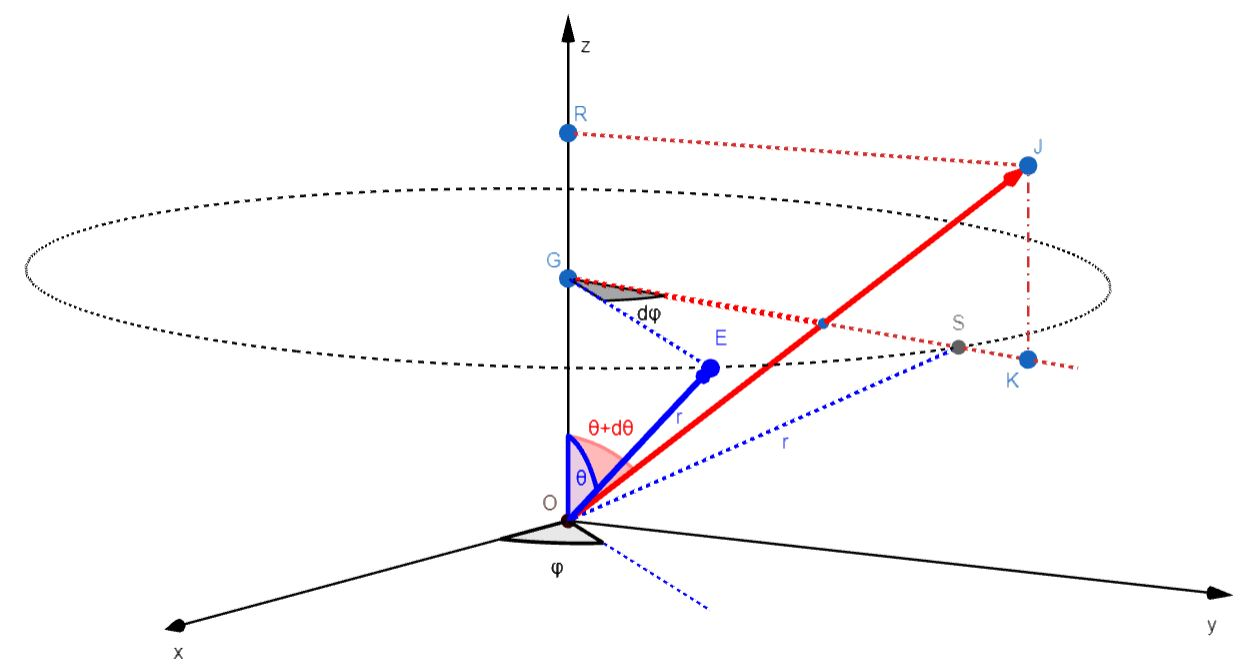
\includegraphics[scale=.6]{sphericalmetric.jpg}\\\\
Consider an infinitesimal displacement of point E to J with $(dr,d\theta, d\phi )$.
\begin{align}
\ ds^2 &= |EJ|^2
\end{align}
As we use infinitesimal displacements we can assume that $$|ES|\perp|GK|\perp|JK|\perp|ES|$$. Hence,
\begin{align}
\ ds^2 = |ES|^2+|SK|^2+|KJ|^2
\end{align}
We have the following relationships
\begin{align}
\left.
\begin{array}{c}
\ |GE| = |GS| = r\sin\theta\\\\
\ |ES| = |GE|d\phi = r\sin\theta d\phi\\\\
\ |GK| = |RJ| = (r+dr)\sin(\theta+d\theta) \\
\ =(r+dr)(\cos(\theta)\sin(d\theta)+\sin(\theta)\cos(d\theta) )\\
\ = (r+dr)(\cos(\theta)d\theta+\sin(\theta))\\
\ = r\cos(\theta)d\theta+r\sin(\theta)+\sin(\theta)dr\\\\
\ |OR| =  (r+dr)\cos(\theta+d\theta)\\
\ = (r+dr)(\cos(\theta)\cos(d\theta)-\sin(\theta)\sin(d\theta))\\
\ = (r+dr)(\cos(\theta)-\sin(\theta)d\theta)\\
\ = r\cos(\theta)-r\sin(\theta)d\theta + \cos(\theta)dr\\\\
\ |OG| = r\cos(\theta)\\\\
\ |JK| = |OR|-|OG| = \cos(\theta)dr-r\sin(\theta)d\theta\\\\
\ |SK| = |GK|-|GS| = r\cos(\theta)d\theta+\sin(\theta)dr\\\\
\end{array}
\right\}
\end{align}
\begin{align}
\left.
\begin{array}{c}
\ |ES|^2 = r^2\sin^2(\theta)d\phi^2\\
\ |SK|^2 = r^2\cos^2(\theta)d\theta^2+\sin^2(\theta)dr^2 +2r\cos(\theta)\sin(\theta)drd\theta \\
\ |JK|^2 = \cos^2(\theta)dr^2+r^2\sin^2(\theta)d\theta^2 -2r\cos(\theta)\sin(\theta)drd\theta\\
\end{array}
\right\}
\end{align}
Hence,
\begin{align}
\ ds^2 &= |ES|^2+|SK|^2+|KJ|^2\\
&= \left\{ \begin{array}{c} r^2\sin^2(\theta)d\phi^2 \\ +r^2\cos^2(\theta)d\theta^2+\sin^2(\theta)dr^2 +2r\cos(\theta)\sin(\theta)drd\theta\\+r^2\sin^2(\theta)d\theta^2+\cos^2(\theta)dr^2 -2r\cos(\theta)\sin(\theta)drd\theta\\
\end{array}
\right.\\
\ &\Rightarrow ds^2= dr^2 + r^2d\theta^2 + r^2\sin^2(\theta)d\phi^2\\
\ & \Rightarrow (a_{mn}) = \begin{pmatrix}
 1& 0 & 0\\
0 & r^2 & 0 \\
0 & 0 & r^2\sin^2\theta \\
\end{pmatrix}
\end{align}
$$\blacklozenge$$
\newpage


\section{p27-exercise}

\begin{tcolorbox}
Starting from 3.103, show that $$a_{mn} = \pdv{y^1}{x^m}\pdv{y^1}{x^n}+\pdv{y^2}{x^m}\pdv{y^2}{x^n}+\pdv{y^3}{x^m}\pdv{y^3}{x^n}$$ and calculate the quantities for a sphere, taking as curvilinear coordinates on he sphere $$x^1 = y^1 , x^2 = y^2$$
\end{tcolorbox}
We have
\begin{align}
\text{(2.103)}\quad &\Rightarrow y^1 = x^1 , y^2 = x^2, y^3 = f^3(x^1,x^2)\\
\text{surface = sphere}\quad &\Rightarrow y^3 = \pm \sqrt{R^2 -(x^1)^2-(x^2)^2}\\
\ ds^2 &= (dx^1)^2+(dx^2)^2+(dx^3)^2\\
\ \text{(1) and (2)}\quad& \Rightarrow \left\{ \begin{array}{c} 
\ dy^1 = dx^1\\\\
\ dy^2 = dx^2\\\\
\ dy^3 = \pm \frac{1}{2} \frac{-2x^1dx^1 - 2x^2dx^2}{\sqrt{R^2 -(x^1)^2-(x^2)^2}}\\\\
\end{array}
\right.\\
\Rightarrow ds^2 & = (dx^1)^2 +  (dx^2)^2 + \frac{(x^1)^2(dx^1)^2 + (x^2)^2(dx^2)^2  + 2 x^1x^2dx^1dx^2}{R^2 -(x^1)^2-(x^2)^2}
\end{align}
\begin{align}
\Leftrightarrow ds^2 & = \frac{(R^2 - (x^2)^2) (dx^1)^2 + (R^2 -(x^1)^2) (dx^2)^2  + 2 x^1x^2dx^1dx^2}{R^2 -(x^1)^2-(x^2)^2}
\end{align}\\
\begin{align}
\Rightarrow (a_{mn}) &= \frac{1}{R^2 -(x^1)^2-(x^2)^2}\begin{pmatrix}
 R^2 - (x^2)^2&x^1x^2 \\
x^1x^2 & R^2 - (x^1)^2 \\
\end{pmatrix}
\end{align}
$$\blacklozenge$$
\newpage


\section{p30-clarification 2.202}

\begin{tcolorbox}
           $$\quad\quad a_{mr}\Delta^{ms} = a_{rm}\Delta^{sm} = \delta^s_r a$$
\end{tcolorbox}
Case 1: $r =s$\\
We have, $a_{Rm}\Delta^{Rm}$ (no summation on R) is the definition of the determinant of A developed along the row R: OK.\\\\
Case 2: $r \neq s$\\
Consider
\begin{align}
\ A &= \begin{pmatrix}
 a_{11} & a_{12}&\dots&a_{1N} \\
a_{21} & a_{22}&\dots&a_{2N} \\
\vdots & \vdots &\vdots & \vdots \\
a_{N1} & a_{N2}&\dots&a_{NN} \\
\end{pmatrix}
\end{align}
and consider the matrix $A^,$
\begin{align}
\ A^, &= \begin{pmatrix}
 a_{11} & a_{12}&\dots&a_{1N} \\
 \vdots & \vdots &\vdots & \vdots \\
a_{R1} & a_{R2}&\dots&a_{RN} \\
\vdots & \vdots &\vdots & \vdots \\
a_{R1} & a_{R2}&\dots&a_{RN} \\
\vdots & \vdots &\vdots & \vdots \\
a_{N1} & a_{N2}&\dots&a_{NN} \\
\end{pmatrix}
\begin{array}{c}
\ \vdots\\
\ \vdots\\
\leftarrow S^{th}\text{ row}\\
\vdots\\
\leftarrow R^{th}\text{ row}\\
\ \vdots\\
\ \vdots\\
\end{array}
\end{align}
This matrix corresponds to the way $a_{Rm}\Delta^{Sm}$ is computed. Indeed with the factor $a_{Rm}$ is not associated it's own cofactor $\Delta^{Rm}$ but the cofactor of the $m^{th}$ column in row $S$. Replacing the $S^{th}$ row with the row $R$ and calculating it's determinant is the same as calculating $a_{Rm}\Delta^{Sm}$\\
But, $|A^,| = 0$ as we have two identical rows. So, $a_{Rm}\Delta^{Sm} = 0$\\\\
Conclusion : The same reasoning can be applied when expanding the determinant along the columns instead of the rows we have indeed $\quad\quad a_{mr}\Delta^{ms} = a_{rm}\Delta^{sm} = \delta^s_r a$.
$$\blacklozenge$$
\newpage


\section{p31-exercise}

\begin{tcolorbox}
Show that if $a{mn} = 0$ for $m\neq n$, then $$a^{11} = \frac{1}{a_{11}}, a^{22} = \frac{1}{a_{22}}, \dots, a¨{12} = 0, \dots$$
\end{tcolorbox}
We have to prove that:
\begin{align}
\ a^{ij} = \left\{\begin{array}{cc}
\frac{1}{a_{ij}} & \text{: }i=j\\
\ 0 & \text{: }i \neq j
\end{array}\right.
\end{align}
From 2.204:
\begin{align}
a_{mR}a_{mS} = \delta^S_R
\end{align}
i) Be $R \neq S$
\begin{align}
\text{(2) }\quad \Rightarrow a_{mR}a_{mS} &= 0\\
\text{but } \quad a_{mR} &=0\quad \forall m \neq R\\
\Rightarrow a_{RR}a^{RS} = 0
\end{align}
but $a_{RR} \neq 0$ ($a_{RR}$ can't be $0$ as the metric tensor would degenerate  if $a_{mn} = 0\quad \forall m \neq n$
\begin{align}
\Rightarrow a^{Rs} = 0\\\\
\end{align}

i) Be $R = S$
\begin{align}
\text{(2) }\quad \Rightarrow a_{mR}a_{mR} &= 1\\
\text{but } \quad a_{mR} &=0\quad \forall m \neq R\\
\Rightarrow a_{RR}a^{RR} = 1\\
\Rightarrow a^{RR} = \frac{1}{a_{RR}}
\end{align}
$$\blacklozenge$$
\newpage

\section{p31-exercise}

\begin{tcolorbox}
Find the components of $a^{mn}$ for spherical polar coordinates in Eulidean 3-space.
\end{tcolorbox}
We have (see exercise page 27):
\begin{align}
\ (a_{mn}) = \begin{pmatrix}
 1& 0 & 0\\
0 & r^2 & 0 \\
0 & 0 & r^2\sin^2\theta \\
\end{pmatrix}
\end{align}
As $a_{mn} = 0 \quad \forall m \neq n$ we deduce (see previous exercise p31)
\begin{align}
\ (a^{mn}) = \begin{pmatrix}
 1& 0 & 0\\
0 & \frac{1}{r^2} & 0 \\
0 & 0 & \frac{1}{r^2\sin^2\theta)}\\
\end{pmatrix}
\end{align}
$$\blacklozenge$$
\newpage

\section{p32-exercise}

\begin{tcolorbox}
Find the mixed metric tensor  $a^{.n}_m$ obtained from $a_{mn}$ by raising the second subscript
\end{tcolorbox}
We have :
\begin{align}
\ a_{i}^{.j} &=  a_{in}a^{nj}\\
\ &=  a_{in}a^{jn}\quad a^{jn} \text{  is symmetric}\\
\ &= \delta^j_i \quad \text{ (see 2.205 pg. 30)}\\
\ &\Rightarrow a_{i}^{.j} = \delta^j_i 
\end{align}
$$\blacklozenge$$
\newpage

\section{p32-clarification 2.214}
\begin{tcolorbox}
          $$ \pdv{a}{a_{mn}} = a a^{mn}$$
\end{tcolorbox}
Put $a_{MN}\equiv a_{mn}$. By definition, we have
\begin{align}
\  a\equiv |a_{mn}|  &= a_{Mk}\Delta^{Mk}\quad\text{(develop determinant along row M)}\\
\ &\Rightarrow \pdv{a}{a_{mn}} = \pdv{a_{Mk}}{a_{mn}}\Delta^{Mk} + a_{Mk}\pdv{\Delta^{Mk}}{a_{mn}}\\
\text{but}\quad &\pdv{a_{Mk}}{a_{mn}} = \left\{\begin{array}{c}
\ 1\quad\text{if} \quad k = N\\
\ 0\quad\text{if} \quad k \neq N\\
\end{array}\right.\\
\text{and}\quad &\pdv{\Delta^{Mk}}{a_{mn}} = 0 \quad \forall k \text{ as } \Delta^{Mk} \text{does not contain the row with } a_{mn} \text{ as element.}\\
\ & \text{(3) and (4)}\quad  \Rightarrow \pdv{a}{a_{mn}} = \Delta^{MN}\\ 
\ &  a^{mn} = \frac{\Delta^{mn}}{a}\quad\text{by definition (see 2.203 page 30)}\\
\ & \Rightarrow \pdv{a}{a_{mn}} = aa^{mn}
\end{align} 
$$\blacklozenge$$
\newpage


\section{p32-exercise}
\begin{tcolorbox}
Prove that $a_{mn}a^{mn} = N$.
\end{tcolorbox}
From 2.204, we have
\begin{align}
\ a_{mr}a^{ms} &= \delta^s_r\\
\text{Consider} \quad a_{mR}a^{mR} &= 1\\
\text{We can repeat (2) for R = 1,2,...,N} \quad \Rightarrow a_{mr}a^{mr} &= N\\
\end{align}
$$\blacklozenge$$
\newpage


\section{p33-exercise}
\begin{tcolorbox}
Show that in Euclidean 3-space with rectangular Cartesian coordinates, the definition 2.301 coincides with the usual definition of the magnitude of a vector.
\end{tcolorbox}
The length of an arbitrary vector in Euclidean 3-space with rectangular Cartesian coordinates, is
\begin{align}
\ ds^2 = (dy^1)^2 + (dy^2)^2 (dy^2)^2
\end {align}
From 2.301, it is obvious that the metrixc tensor can be expressed as,
\begin{align}
\begin{pmatrix}1 & 0 &0 \\ 0 & 1 &0\\0 & 0 &1  \\ \end{pmatrix} 
\end{align}
$$\blacklozenge$$
\newpage


\section{p34-exercise}
\begin{tcolorbox}
A curve in Euclidean 3-space has the equations $$ x^1 =  a \cos(u), x^2 = a\sin(u), x^3 = bu$$ where $x^1, x^2,x^3$ are rectangular Cartesian coordinates,$u$ is a parameter, and $a, b$ are positive constants. Find the length of this curve between the point $u = 0$ and $u = 2\pi$.
\end{tcolorbox}
The metric tensor has the following form,
\begin{align}
\ (a_{ij}) &= \begin{pmatrix}1 & 0 &0 \\ 0 &1 &0\\0 & 0 &1  \\ \end{pmatrix} \\
\text {and  (2.306)  }\quad s &= \int^{2\pi}_0[\epsilon a_{mn}p^mp^n]^{\frac{1}{2}}du
\end{align}
with
\begin{align}
\ p^1 = \dv{x^1}{u} = -a\sin(u), \quad p^2 = \dv{x^2}{u} = a\cos(u), \quad p^3 = \dv{x^3}{u} = b
\end{align}
Hence (2) becomes
\begin{align}
s &= \int^{2\pi}_0\epsilon[a^2 \sin^2(u) + a^2\cos^2(u) + b^2]^{\frac{1}{2}}du\\
\ &= \int^{2\pi}_0\epsilon[a^2+  b^2]^{\frac{1}{2}}du\\
\ &= [a^2+  b^2]^{\frac{1}{2}} \left. u\right|^{2\pi}_0\\
\ &= 2\pi[a^2+  b^2]^{\frac{1}{2}} 
\end{align}
$$\blacklozenge$$
\newpage

\section{p36-clarification 2.314}
\begin{tcolorbox}
Going from 2.313 to 2.314 yields because both $X^m$ and $Y^m$ are unit vectors and by definition of the magnitude (see 2.301) both  $a_{mn}X^mX^n$ and $a_{mn}Y^mY^n$ are 1 (also due to the fact that only a positive definite metric tensor is considered, $\epsilon = 1$).
\end{tcolorbox}
$$\blacklozenge$$
\newpage

\section{p37-exercise}

\begin{tcolorbox}
Show that the small angle between unit vectors $X^r$ and $X^r + dX^r$ (these increments being infenitesimal) is given by $$ \theta^2 = a_{mn}X^mX^n$$
\end{tcolorbox}
\begin{figure}[htp]  

    \centering
 
%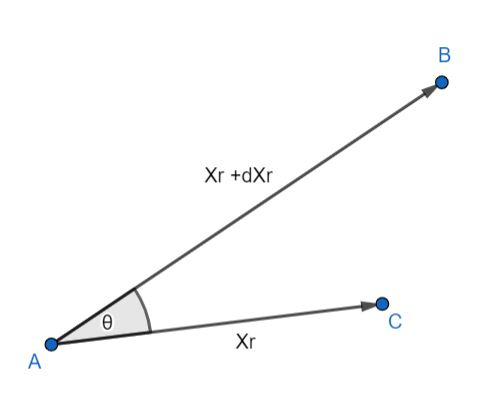
\includegraphics[scale=.5]{Exp37_1.jpg}
\begin{tikzpicture}[yscale=-0.3,xscale=0.3]
%uncomment if require: \path (0,300); %set diagram left start at 0, and has height of 300
\coordinate [label=left:$A$] (A) at (12.116,21.364);
\coordinate [label=above right:$B$] (B) at (32.688,1.187);
\coordinate  [label=above right:$C$] (C) at (34.06,14.021);

%\draw (A) --(C) node[midway,below] {$X_r $};
%\draw (A) --(B) node[midway,above,left] {$X_r+dX_r \quad$};
\draw[ -stealth,line width = 0.25mm] (A) --(C) node[midway,below] {$X_r $};
\draw[ -stealth,line width = 0.25mm] (A) --(B) node[midway,above,left] {$X_r+dX_r \quad$};
\draw (A)  circle[radius=4pt];
\draw pic[draw,angle radius=2cm,"$\theta$" shift={(3mm,3mm)}] {angle=C--A--B};
\end{tikzpicture}\\
\caption{Small angle expression}
\end{figure}
By definition (2.302 page 33)
\begin{align} 
\ |BC|^2 =\epsilon a_{mn}dX^mdX^n\\
\end{align}
We can drop $\epsilon = 1$ as the considered space is positive definite.\\
As $\theta$ is infinitesimal, we can state
\begin{align}
\ |BC| &\approx |AC|\theta\\
\text{ and } \quad |AC| &= X^r = 1\quad  \text{(as } X^r \text{ is a unit vector)}\\
\Rightarrow \theta^2 &= a_{mn}dX^mdX^n
\end{align}
$$\blacklozenge$$
\newpage


\section{p39-clarification 2.409}

\begin{tcolorbox}
We clarify the integration by parts in the derivation of the general  geodesic equation.
\end{tcolorbox}
We have 
\begin{align}
\int d(A.B) &= \int AdB + \int BdA\\
\Rightarrow  \int AdB &= \int BdA -  \int d(A.B)\
\end{align}
Now, substitute 2.407 in 2.406, we get
\begin{align}
\dv{L}{v} &= \int \pdv{(\epsilon w)^{\frac{1}{2}}}{x^r} \pdv{x^r}{v} du +  \int \pdv{(\epsilon w)^{\frac{1}{2}}}{p^r} \pdv{p^r}{v} du\\
\ &= \int \pdv{(\epsilon w)^{\frac{1}{2}}}{x^r} \pdv{x^r}{v} du +  \int \pdv{(\epsilon w)^{\frac{1}{2}}}{p^r} \pdv{\pdv{x^r}{v}}{u} du\\
&= \int \pdv{(\epsilon w)^{\frac{1}{2}}}{x^r} \pdv{x^r}{v} du +  \int \pdv{(\epsilon w)^{\frac{1}{2}}}{p^r} d(\pdv{x^r}{v})
\end{align}
To integrate by parts the second term in (5) we put in (2)
$$A= \pdv{(\epsilon w)^{\frac{1}{2}}}{p^r} \quad \text{and } B = \pdv{x^r}{v}$$
\begin{align}
\int \pdv{(\epsilon w)^{\frac{1}{2}}}{p^r} d(\pdv{x^r}{v}) &= \int AdB \\
\ & = \int BdA -  \int d(A.B)\\
\ &= \pdv{(\epsilon w)^{\frac{1}{2}}}{p^r}\left.\pdv{x^r}{v}\right|_{u_0}^{u_1} - \int \pdv{x^r}{v}d(\pdv{(\epsilon w)^{\frac{1}{2}}}{p^r} )\\
\ &= \pdv{(\epsilon w)^{\frac{1}{2}}}{p^r}\left.\pdv{x^r}{v}\right|_{u_0}^{u_1} - \int \pdv{x^r}{v}\pdv{\pdv{(\epsilon w)^{\frac{1}{2}}}{p^r} )}{u}du
\end{align}
Replacing (9) in (5) gives the formulea 2.409.
$$\blacklozenge$$
\newpage

\section{p41-exercise}
\begin{tcolorbox}
Prove the following identities: $$ [mn,r] = [nm,r], \quad [rm,n]+[rn,m] = \partial_r a_{mn}$$
\end{tcolorbox}
\begin{align}
\ [mn,r] &= \frac{1}{2}(\partial_{n} a_{mr}+ \partial_{m} a_{nr} - \partial_{r} a_{mn})\\
\ &= \frac{1}{2}(\partial_{m} a_{nr} + \partial_{n} a_{mr}  - \partial_{r} a_{nm})\\
\ &=[nm,r] 
\end{align}
and 
\begin{align}
\ [rm,n] + [rn,m]&= \frac{1}{2}(\partial_{r} a_{mn}+ \partial_{m} a_{rn} - \partial_{n} a_{rm} + \partial_{n} a_{rm}+ \partial_{r} a_{mn} - \partial_{m} a_{rn})\\
\ &= \frac{1}{2}(\partial_{r} a_{mn}+\partial_{r} a_{mn})\\
\ &=\partial_{r} a_{mn}
\end{align}
$$\blacklozenge$$
\newpage

\section{p42-exercise}
\begin{tcolorbox}
Prove that  $$ [mn,r] = a_{rs}\Gamma^s_{mn}$$
\end{tcolorbox}
\begin{align}
\ a_{rs}\Gamma^s_{mn} & = a_{rs}a^{sk}[mn,k]\\
\ & = \delta^k_r[mn,k]\\
\ &= [mn,r]
\end{align}
$$\blacklozenge$$
\newpage

\section{p42-clarification on 2.430}
\begin{tcolorbox}
... This may proved without difficulty by starting with 2.427, in which $\lambda$ is a known function of $u$ , and defining $s$ by the relation$$ s = \int^u_{u_0}(exp\int^v_{v_0} \lambda(w)dw)dv$$ $u_0, v_0$ being constants....
\end{tcolorbox}
\begin{align}
\text{see 2.428 :} \quad  \lambda (u)=-\frac{\dv[2]{u}{s}}{(\dv{u}{s})^2}\\
\end{align}
We suppose $u(s)$ continuous by parts with continuous inverse.
\begin{align}
\Rightarrow \dv{s}{u} &= \frac{1}{\dv{u}{s}}\\
\Rightarrow \dv[2]{s}{u}&= \dv{(\frac{1}{\dv{u}{s}})}{s}\dv{s}{u}\\
\ & = -\frac{\dv[2]{u}{s}}{(\dv{u}{s})^2}\dv{s}{u}\\
\Rightarrow \frac{\dv[2]{s}{u}}{\dv{s}{u}} &= - \frac{\dv[2]{u}{s}}{(\dv{u}{s})^2}  
\end{align}
By definition (2.428)
\begin{align}
\ \lambda (u) &= - \frac{\dv[2]{u}{s}}{(\dv{u}{s})^2}\\
\text{hence by (6) and (7):}\quad  \lambda (u) &= \frac{\dv[2]{s}{u}}{\dv{s}{u}}\\
\text{in (8) put}\quad y &= \dv{s}{u} \\
\text{ and so} \quad \lambda (w)  &= \frac{y^,}{y}\\
\Rightarrow \int \frac{y^,}{y}dw &= \int \lambda (w)dw\\
\Leftrightarrow \int d(lny) &= \int \lambda (w)dw\\
\Rightarrow \left. ln(y) \right|^v_{v_0} &= \int^v_{v_0} \lambda (w)dw\\
\Rightarrow y  &= exp(\int^v_{v_0} \lambda (w)dw) + C
\end{align}
Taking into account (9), we get:
\begin{align}
\dv{s}{v}  &= exp(\int^v_{v_0} \lambda (w)dw) + C\\
\Rightarrow \left. s \right|^u_{u_0} &=\int^u_{u_0}  exp(\int^v_{v_0} \lambda (w)dw)dv +Cu + B^,\\
\Leftrightarrow  s  &=\int^u_{u_0}  exp(\int^v_{v_0} \lambda (w)dw)dv +Cu + B
\end{align}
We show tha we have to put $C=0$ and can drop the constant $B$. Remember by (8)
\begin{align}
\lambda (u) &= \frac{\dv[2]{s}{u}}{\dv{s}{u}}\\
\text{by (17)} \quad \dv{s}{u}  &=exp(\int^u_{u_0} \lambda (w)dw) +C\\
\text{and}\quad \dv[2]{s}{u}  &= \lambda (u) exp(\int^u_{u_0} \lambda (w)dw) \\
\text{hence by (18), (19) and (20):} \quad \lambda (u)&= \frac{\lambda (u) exp(\int^u_{u_0} \lambda (w)dw)}{exp(\int^u_{u_0} \lambda (w)dw) +C}
\end{align}
So, whatever the constant B, the relation (18) is correct on the condition that C=0. 
So, indeed, we can choose the independent variable $s$ as
$$s  =\int^u_{u_0}  exp(\int^v_{v_0} \lambda (w)dw)dv $$ 
$$\blacklozenge$$
\newpage

\section{p42-clarification on 2.430}
\begin{tcolorbox}
After 2.430 it is stated:\\
\it{"No matter what values these constants have, 2.424 is satisfied, and by adjusting the constant $v_0$, we can ensure that $a_{mn}\dv{x^m}{s}\dv{x^n}{s} = \pm1$ along $C$, so that $s$ is actually the arc length."}
\end{tcolorbox}
We first prove that 2.4.24 is satisfied, no matter what values the constants take. We have
\begin{align}
\text{(2.430) } \quad  &s =\int_{u_0}^u(exp\int_{v_0}^v \lambda (w)dw)dv\\
\text{and (2.427)} \quad &\dv[2]{x^r}{u} + \Gamma^r_{mn}\dv{x^m}{u}\dv{x^n}{u} =  \lambda \dv{x^r}{u}
\end{align}
In (2) we can write the first term as
\begin{align}
\quad \dv[2]{x^r}{u} &= \dv{(\dv{x^r}{u})}{s}\dv{s}{u} \\
\text{with } \quad \dv{(\dv{x^r}{u})}{s} &=  \dv{(\dv{x^r}{s}\dv{s}{u})}{s} = \dv[2]{x^r}{s}\dv{s}{u}+\dv{x^r}{s}\dv{(\dv{s}{u})}{s} 
\end{align}
Assuming the curve smooth, we have
\begin{align}
\dv{(\dv{s}{u})}{s} & = \dv{(\frac{1}{\dv{u}{s}})}{s} = -\frac{\dv[2]{u}{s}}{(\dv{u}{s})^2}= \lambda
\end{align}
Putting (4) and (5) in (3) we get
\begin{align}
\dv[2]{x^r}{u} &= \dv[2]{x^r}{s} \left ( \dv{s}{u}\right )^2 + \lambda\dv{x^r}{s}\dv{s}{u}
\end{align}
Plugging (6) in 2.427 gives:
\begin{align}
\dv[2]{x^r}{s} \left (\dv{s}{u}\right )^2 + \lambda\dv{x^r}{s}\dv{s}{u} +\Gamma^r_{mn}\dv{x^m}{s}\dv{x^n}{s}\left (\dv{s}{u}\right )^2  &=  \lambda \dv{x^r}{s}\dv{s}{u}\\
\Leftrightarrow \dv[2]{x^r}{s} \left (\dv{s}{u}\right )^2 +\Gamma^r_{mn}\dv{x^m}{s}\dv{x^n}{s}\left (\dv{s}{u}\right )^2  &=  0
\end{align}
We can assume that $\dv{s}{u} $ does not become $0$ or $\pm \infty$ along the curve by choosing an adequate constant $v_0$. Indeed, from (2.430) we get
\begin{align}
\dv{s}{u}  &= exp(\int_{u_0}^u \lambda (w)dw)\\
\ &= \frac{\phi (u)}{\phi (u_0)}
\end{align}
with $\phi (u_0) =  e^{\theta(u_0)}$, $\theta(u)$ being the indefinite integral $\int \lambda (w)dw $.\\
So, it is sufficient to choose $v_0$ so that $\theta(u_0)$ does not become  $\pm \infty$ to ensure that $\dv{s}{u} \ne 0$ or $ \ne \pm \infty$ along the curve and so we have from (8)
\begin{align}
\dv[2]{x^r}{s} +\Gamma^r_{mn}\dv{x^m}{s}\dv{x^n}{s}  &=  0\end{align}
which is the definition (2.424) of a geodesic.\\\\
The same reasoning about $\dv{s}{u} \ne 0$ can be made to prove that $a_{mn}\dv{x^m}{s}\dv{x^n}{s} = \pm1$ along $C$. Indeed, by definition (2.305):
\begin{align}
\ ds = &\left[ \epsilon a_{mn}\dv{x^m}{u}\dv{x^n}{u}\right]^\frac{1}{2}\\
\text{ equating with (9)} \quad   &\left[ \epsilon a_{mn}\dv{x^m}{u}\dv{x^n}{u}\right]^\frac{1}{2} =                 exp(\int_{u_0}^u \lambda (w)dw)\\
\Rightarrow \quad &\epsilon a_{mn}\dv{x^m}{s}\dv{x^n}{s}\left (\dv{s}{u}\right )^2 =  \left[ exp(\int_{u_0}^u \lambda (w)dw) \right]^2\\
\text{but} \quad &\dv{s}{u} = exp(\int_{u_0}^u \lambda (w)dw)\\
\text{ and so, (9) becomes} \quad &\epsilon a_{mn}\dv{x^m}{s}\dv{x^n}{s}\left (\dv{s}{u}\right )^2 =  \left (\dv{s}{u}\right )^2\\
\Rightarrow \quad & a_{mn}\dv{x^m}{s}\dv{x^n}{s}=\epsilon
\end{align}
$$\blacklozenge$$
\newpage


\section{p43-clarification }
\begin{tcolorbox}
$$\lambda = \Gamma^N_{\mu \nu}\dv{x^{\mu}}{x^N} \dv{x^{\nu}}{x^N} + 2\Gamma^N_{\mu N}\dv{x^{\mu}}{x^N}+\Gamma^N_{N N} $$
\end{tcolorbox}
We start with 2.427 with $r=N$
\begin{align}
\ &\dv[2]{x^N}{{x^{N}}} + \Gamma^N_{\mu\nu}\dv{x^{\mu}}{x^N} \dv{x^{\nu}}{x^N} = \lambda \dv{x^N}{x^N}\\
\Rightarrow\quad &\Gamma^N_{\mu\nu}\dv{x^{\mu}}{x^N} \dv{x^{\nu}}{x^N} = \lambda \quad \text{(as}\quad \dv[2]{x^N}{{x^{N}}} = 0 \quad \dv{x^N}{x^N} = 1 \text{)}
\end{align}
But (2) is only valid with the dummy indices $\mu$ and $\nu$ spanning the whole dimension $(1,2,\dots N)$, but by choice $\mu,\nu \quad \epsilon \quad (1,2, \dots, N-1)$. We have thus to add in the left term of (2) the cases
\begin{align}
\left\{ \begin{array}{cc}
\Gamma^N_{N\nu}& \nu = (1,2,\dots ,N-1)\\\\
\Gamma^N_{\mu N}& \mu = (1,2,\dots ,N-1)\\\\
\Gamma^N_{NN}& \\
\end{array} \right.\\
\text{(2) becomes } \quad \Gamma^N_{\mu\nu}\dv{x^{\mu}}{x^N} \dv{x^{\nu}}{x^N} + \Gamma^N_{N \nu}\dv{x^N}{x^N} \dv{x^{\nu}}{x^N} + \Gamma^N_{\mu N}\dv{x^{\mu}}{x^N} \dv{x^{N}}{x^N} + \Gamma^N_{NN}\dv{x^{N}}{x^N} \dv{x^{N}}{x^N}= \lambda\\
\Rightarrow   \quad \Gamma^N_{\mu\nu}\dv{x^{\mu}}{x^N} \dv{x^{\nu}}{x^N} + \Gamma^N_{N \nu}\dv{x^{\nu}}{x^N} + \Gamma^N_{\mu N}\dv{x^{\mu}}{x^N}+ \Gamma^N_{NN} = \lambda
\end{align}
As $\Gamma^N_{\mu N}$ is symmetric on the lower indices and $\mu$, $\nu$ being dummy indices:
\begin{align}
\lambda  =\Gamma^N_{\mu\nu}\dv{x^{\mu}}{x^N} \dv{x^{\nu}}{x^N} + 2\Gamma^N_{N \nu}\dv{x^{\nu}}{x^N} +\Gamma^N_{NN}
\end{align}
The other $N-1$ equation for $r= 1,\dots, N-1$ can be deduced following the same reasoning.
$$\blacklozenge$$
\newpage


\section{p45-clarification }
\begin{tcolorbox}
$ f_r \equiv a_{rm}\dv[2]{x^m}{u} +[mn,r]\dv{x^m}{u}\dv{x^n}{u}$ is covariant and 
$ f^r \equiv \dv[2]{x^m}{u} +\Gamma^r_{mn}\dv{x^m}{u}\dv{x^n}{u}$ is contravariant.
\end{tcolorbox}
\begin{align}
\ &f_r \equiv a_{rm}\dv[2]{x^m}{u} +[mn,r]\dv{x^m}{u}\dv{x^n}{u}\\
\text{multiply with}\quad a^{sr}\quad \Rightarrow\quad &f_r a^{sr} = a^{sr}a_{rm}\dv[2]{x^m}{u} +a^{sr}[mn,r]\dv{x^m}{u}\dv{x^n}{u}\\
\Rightarrow\quad &f^{s} = \delta^s_m \dv[2]{x^m}{u} +\underbrace{a^{sr}[mn,r]}_{\Gamma^s_{mn}}\dv{x^m}{u}\dv{x^n}{u}\\
\Rightarrow \quad &f^{s} = \dv[2]{x^s}{u} +\Gamma^s_{mn}\dv{x^m}{u}\dv{x^n}{u}
\end{align}
By lifting the index of $f_r$ we get a contravariant vector confirming that (4) is contravariant.
$$\blacklozenge$$
\newpage

\section{p45-clarification }
\begin{tcolorbox}
(2.443) and (2.444)
$$ p^r\pdv{w}{p^r} - w = C^t \quad \Rightarrow\quad w = C^t $$ 
\end{tcolorbox}
By definition 
\begin{align}
\ w &= a_{mn}p^mp^n\\
\Rightarrow\quad \pdv{w}{p^r} &= a_{mn}(\pdv{p^m}{p^r}p^n + p^m \pdv{p^n}{p^r})\\
\ &= a_{mn}(\delta^m_rp^n + p^m \delta^n_r)\\
\ &= a_{rn}p^n + a_{mr}p^m \\
\ &= 2a_{mr}p^m \quad\text{(as } a_{mn} \quad \text{is symmetric)}\\
\text{(4)}\quad \Rightarrow \quad p^r\pdv{w}{p^r} &= 2a_{mr}p^rp^m \\
\ &= 2w\\
\text{(2.443)} \quad\Rightarrow\quad p^r\pdv{w}{p^r} -w &= 2w-w = w = C^t\\
\Rightarrow\quad w &\equiv a_{mn}p^mp^n = C^t
\end{align}
$$\blacklozenge$$
\newpage


\section{p47-exercise }
\begin{tcolorbox}
The class of all parameters $u$, for which the equations of a geodesic null line assume the simple form 2.445, are obtained from any one such parameter by linear transformation $$ \overline{u} = au + b$$ $a$ and $b$ being constants.
\end{tcolorbox}
The simple form 2.445 is :
\begin{align}
\  \dv[2]{x^r}{u} +\Gamma^r_{mn}\dv{x^m}{u}\dv{x^n}{u} = 0\\
\end{align}
The general form of a geodesic is (2.447) 
\begin{align}
\  \dv[2]{x^r}{\overline{u}} +\Gamma^r_{mn}\dv{x^m}{\overline{u}}\dv{x^n}{\overline{u}} = \lambda \dv{x^r}{\overline{u}}\\
\end{align}
So (2.447) can only of the form (2.445) if $\lambda = 0$
\begin{align}
\   \lambda  = - \frac{\dv[2]{\overline{u}}{u}}{\left( \dv{\overline{u}}{u}\right)^2} = 0\\
\end{align}
We can state that $\dv{\overline{u}}{u}\ne 0$ as $\overline{u}$ can't be a constant (being a parameter of a curve). So,
\begin{align}
\dv[2]{\overline{u}}{u}&=0\\
\Rightarrow \quad \dv{\overline{u}}{u}&=a\\
\Rightarrow \quad \overline{u}&=au +b
\end{align}
$$\blacklozenge$$
\newpage

\section{p47-exercise }
\begin{tcolorbox}
Consider a 3-space with coordinates $x,y,z$ and a metric form $\Phi = (dx)^2+(dy)^2 - (dz)^2$. prove that the geodesic null lines may be represented by the equations
$$x = au + a^,\quad y = bu + b^, \quad z = cu + c^,$$
where $u$ is a parameter and $a, a^,,b,b^,,c,c^,$ are constants which are arbitrary except for the relation $a^2+b^2-c^2 =0$.
\end{tcolorbox}
Given is 
\begin{align}
\Phi = (dx)^2+(dy)^2 - (dz)^2
\end{align}
From the previous exercise we have already proven that $x,y,z$ are of the form
\begin{align}
\ x^i = q_i u + q_i^,
\end{align}
To be a null geodesic null line we need to have (2.448)
\begin{align}
\ a_{mn}\dv{x^m}{u}\dv{x^n}{u} &=0\\
\text{from (1) we deduce}  \quad (a_{mn}) &= \begin{pmatrix}
1& 0 & 0 \\
 0&1  & 0 \\
 0&  0& -1 \\
\end{pmatrix}\\
\text{(3)}\quad\Rightarrow\quad (dx)^2+(dy)^2 - (dz)^2 &=0\\
\text{(2)}\quad\Rightarrow\quad (q_1)^2+(q_2)^2 - (q_3)^2 &=0
\end{align}
$$\blacklozenge$$
\newpage

\section{p48-exercise }
\begin{tcolorbox}
Prove that the Christoffel symbols of the first kind transform according the equation 
$$[mn,r]^, =  [pq,s]\pdv{x^p}{x^{,m}} \pdv{x^q}{x^{,n}}\pdv{x^s}{x^{,r}}+ a_{pq}\pdv{x^p}{x^{,r}}\pdv{x^q}{x^{,m}}{x^{,n}}$$
\end{tcolorbox}
From 2.438 page 45, we have
\begin{align}
\ f_r &\equiv a_{rm}\dv[2]{x^m}{u} +[mn,r]\dv{x^m}{u}\dv{x^n}{u} \quad\text{is covariant} \\
\Rightarrow\quad f_r^, &= f_s\pdv{x^s}{x^{,r}}\\
\text{with}\quad f_r^, &= a^,_{rm}\dv[2]{x^{,m}}{u} +[mn,r]^, \dv{x^{,m}}{u}\dv{x^{,n}}{u}
\end{align}
Combining (1), (2) and (3) gives 
\begin{align}
\ a^,_{rm}\dv[2]{x^{,m}}{u} +[mn,r]^, \dv{x^{,m}}{u}\dv{x^{,n}}{u} = ( a_{sm}\dv[2]{x^m}{u} +[mn,s]\dv{x^m}{u}\dv{x^n}{u})\pdv{x^s}{x^{,r}}
\end{align}
We rewrite (4) as 
\begin{align}
\ [mn,r]^, \dv{x^{,m}}{u}\dv{x^{,n}}{u} &= -\underbrace{a^,_{rm}\dv[2]{x^{,m}}{u}}_\text{(*)} +\underbrace{ a_{sm}\dv[2]{x^m}{u}\pdv{x^s}{x^{,r}}}_\text{(**)} +\underbrace{[mn,s]\dv{x^m}{u}\dv{x^n}{u}\pdv{x^s}{x^{,r}}}_\text{(***)}\\
\text{(***)} &\Leftrightarrow [mn,s]\pdv{x^m}{x^{,p}}\dv{x^{,p}}{u}\pdv{x^n}{x^{,q}}\dv{x^{,q}}{u}\pdv{x^s}{x^{,r}}
\end{align}
In (6) renaming the dummy indices $m,n,p,q$ gives
\begin{align}
\text{(***)} &\Leftrightarrow [pq,s]\pdv{x^p}{x^{,m}}\dv{x^{,m}}{u}\pdv{x^q}{x^{,n}}\dv{x^{,n}}{u}\pdv{x^s}{x^{,r}}\\
&\Leftrightarrow [pq,s]\pdv{x^p}{x^{,m}}\pdv{x^q}{x^{,n}}\pdv{x^s}{x^{,r}}\left(\dv{x^{,m}}{u}\dv{x^{,n}}{u}\right)
\end{align}
Also,
\begin{align}
\text{(**)} &\Leftrightarrow  a_{sm}\dv[2]{x^m}{u}\pdv{x^s}{x^{,r}}\\
\text{As we have also}\quad \dv[2]{x^m}{u} &= \dv{(\pdv{x^m}{x^{,p}}\dv{x^{,p}}{u})}{u}\\
&= \pdv{x^m}{x^{,p}}\dv[2]{x^{,p}}{u}+\dv{x^{,p}}{u}\pdv{x^m}{x^{,p}}{x^{,q}}\dv{x^{,q}}{u} 
\end{align}
(11) and (9) gives by changing the dummy indices ( $m\rightarrow t$, $p\rightarrow m$, $q\rightarrow n$)
\begin{align}
\text{(**)}&= \underbrace{a_{st}\pdv{x^t}{x^{,p}}\dv[2]{x^{,p}}{u}\pdv{x^s}{x^{,r}}}_\text{(****)}+a_{pq}\pdv{x^q}{x^{,m}}{x^{,n}}\pdv{x^{p}}{x^{,r}}\left(\dv{x^{,m}}{u}\dv{x^{,m}}{u}\right) \\
\text{with (****)}\quad &= a_{st}\left(\pdv{x^t}{x^{,m}}\pdv{x^s}{x^{,r}}\right)\dv[2]{x^{,m}}{u}
\end{align}
But $a_{st}$  is a covariant tensor, so
\begin{align}
\ a^{,}_{rm} &= a_{st}\pdv{x^t}{x^{,m}}\pdv{x^s}{x^{,r}}\\
\text{(13) becomes}\quad \text{(****)} &= a^{,}_{rm}\dv[2]{x^{,m}}{u}\\
\text{and from (5) we have }\quad \text{(*)} &= -a^{,}_{rm}\dv[2]{x^{,m}}{u}\\
\end{align}
and both terms cancel each other in equation (5). So adding $(*), (**)$ and $(***)$ in (5) , we get 
\begin{align}
\ [mn,r]^, \dv{x^{,m}}{u}\dv{x^{,n}}{u} &= a_{pq}\pdv{x^q}{x^{,m}}{x^{,n}}\pdv{x^{p}}{x^{,r}}\left(\dv{x^{,m}}{u}\dv{x^{,m}}{u}\right)+[pq,s]\pdv{x^p}{x^{,m}}\pdv{x^q}{x^{,n}}\pdv{x^s}{x^{,r}}\left(\dv{x^{,m}}{u}\dv{x^{,n}}{u}\right)\\
\Rightarrow \ &[mn,r]^, =[pq,s]\pdv{x^p}{x^{,m}}\pdv{x^q}{x^{,n}}\pdv{x^s}{x^{,r}}+  a_{pq}\pdv{x^{p}}{x^{,r}}\pdv{x^q}{x^{,m}}{x^{,n}}
\end{align}
$$\blacklozenge$$
\newpage

\section{p50-clarification 2.515 }
\begin{tcolorbox}
$$\dv{\left(T_rS^r\right)}{u} = \dv{T_r}{u}S^r + T_r\dv{S^r}{u} = \left(\dv{T_r}{u} - \Gamma^m_{rn}T_m\dv{x^n}{u}\right)S^r$$ with $$\frac{\delta T_r}{\delta u} = \dv{T_r}{u} -\Gamma^m_{rn}\dv{x^n}{u} T_m$$ a covariant vector.
\end{tcolorbox}
It is given that $S^r$ is a tensor propagated parallelly along the curve. The by (2.5212) we have
\begin{align}
\dv{S^r}{u} &+ \Gamma^r_{mn}S^m\dv{x^n}{u}= 0\\
\dv{S^r}{u} &= - \Gamma^r_{mn}S^m\dv{x^n}{u}\\
\text{and}\quad \dv{\left(T_rS^r\right)}{u} &= \dv{T_r}{u}S^r + T_r\dv{S^r}{u} \\
\ &= \dv{T_r}{u}S^r -\Gamma^r_{mn}S^m\dv{x^n}{u} T_r\\
\end{align}
Swap dummy indices $r$ and $m$ in the second term:
\begin{align}
\dv{\left(T_rS^r\right)}{u} &= \dv{T_r}{u}S^r -\Gamma^m_{rn}S^r\dv{x^n}{u} T_m\\
\ &= \left(\dv{T_r}{u} -\Gamma^m_{rn}\dv{x^n}{u} T_m\right)S^r\\
\end{align}
As $T_rS^r$ is an invariant and thus is also $\dv{\left(T_rS^r\right)}{u}$ and as $S^r$ can be chosen arbitrarily (as long it is a contravariant tensor), implies that $$\dv{T_r}{u} -\Gamma^m_{rn}\dv{x^n}{u} T_m$$ is covariant and thus also $$\frac{\delta T_r}{\delta u} = \dv{T_r}{u} -\Gamma^m_{rn}\dv{x^n}{u} T_m$$
$$\blacklozenge$$
\newpage

\section{p50-clarification 2.516}
\begin{tcolorbox}
$$\frac{\delta T_{rs}}{\delta u} \equiv \dv{T_{rs}}{u}  - \Gamma^m_{rn}T_{ms}\dv{x^n}{u} - \Gamma^m_{sn}T_{rm}\dv{x^n}{u}$$ is a covariant vector.
\end{tcolorbox}
We build an invariant $ T_{rs} S^rU^s$ with $S^r$ and $U^s$ arbitrary contravariant tensors. The we know that $\dv{\left( T_{rs} S^r U^s\right)}{u}$ is also an invariant. We have 
\begin{align}
\dv{\left( T_{rs} S^r U^s\right)}{u} = \dv{T_{rs}}{u} S^r U^s + T_{rs} \dv{S^r}{u} U^s + T_{rs} S^r \dv{U^s}{u}
\end{align} 
with with $S^r$ and $U^s$ propagated parallelly along the curve. Then,
\begin{align}
\dv{S^r}{u} = - \Gamma^r_{mn}S^m\dv{x^n}{u}\\
\dv{U^s}{u} = - \Gamma^s_{mn}Y^m\dv{x^n}{u}
\end{align} 
(2), (3) in (1) gives 
\begin{align}
\dv{\left( T_{rs} S^r U^s\right)}{u} = \dv{T_{rs}}{u} S^r U^s - T_{rs}U^s\Gamma^r_{mn}S^m\dv{x^n}{u} - T_{rs} S^r \Gamma^s_{mn}U^m\dv{x^n}{u}
\end{align} 
Changing the dummy indices in the second and third term gives:
\begin{align}
\dv{\left( T_{rs} S^r U^s\right)}{u} = (\dv{T_{rs}}{u}  - \Gamma^m_{rn}T_{ms}\dv{x^n}{u} - \Gamma^m_{sn}T_{rm}\dv{x^n}{u})S^r U^s
\end{align} 
As the left term is an invariant and $S^r$ and $U^s$ are arbitrary contravariant tensors, means that the expression in the brackets in the right part of the equation, is a covariant tensor.
$$\blacklozenge$$
\newpage

\section{p51-exercise}
\begin{tcolorbox}
Find the absolute derivative of $T^r_{st}$.
\end{tcolorbox}
Define the invariant $ I = D^r_{st}R^rS_sT_t$ 
\begin{align}
\ I &= D^r_{st}R^rS_sT_t\\
\Rightarrow A &= \dv{I}{u}= 
\dv{\left(D^r_{st}\right)}{u}R^rS_sT_t+
\ D^r_{st}S_sT_t\dv{\left(R^r\right)}{u}+
\ D^r_{st}R_rT_t\dv{\left(S^s\right)}{u}+
\ D^r_{st}R_rS_s\dv{\left(T^t\right)}{u}
\end{align} 
Reminder, performing a parallel propagation of a covariant and contravariant vector gives as equations
\begin{align}
\dv{V^v}{u} = - \Gamma^v_{mn}V^m\dv{x^n}{u}\\
\dv{W_w}{u} = + \Gamma^m_{wn}W^m\dv{x^n}{u}
\end{align}
So (2) becomes:
\begin{align}
\ A = \left\{ \begin{array}{c}
\dv{\left(D^r_{st}\right)}{u}R^rS_sT_t\\\\
\ -D^r_{st}S_sT_t\Gamma^r_{mn}R^m\dv{x^n}{u}\\\\
\ +D^r_{st}R_rT_t \Gamma^m_{sn}S^m\dv{x^n}{u}\\\\
\ +D^r_{st}R_rS_s\Gamma^m_{tn}T^m\dv{x^n}{u}
\end{array} \right.
\end{align}
In (5) apply the following renaming of dummy variables 
$$\left\{\begin{array}{c}
2^{nd} line: \quad r\rightarrow m, m \rightarrow r\\
3^{rd} line: \quad s\rightarrow m, m \rightarrow s\\
4^{th} line: \quad t\rightarrow m, m \rightarrow t\\
\end{array}  \right. $$
and regrouping terms with $R^rS_sT_t$,(5) becomes then
\begin{align}
\ A = \left[\dv{\left(D^r_{st}\right)}{u}+(\ D^r_{mt}\Gamma^s_{mn}+\ D^r_{sm}\Gamma^t_{mn}-\ D^m_{st}\Gamma^m_{rn})\dv{x^n}{u}\right]R^rS_sT_t
\end{align}
But $A$ is an invariant, so the expression in the square parenthesis is a tensor of the form $T^r_{st}$ and we define the absolute derivative of $T^r_{st}$ as:
$$ \frac{\delta T^r_{st}}{\delta u} = \dv{\left(T^r_{st}\right)}{u}+\Gamma^s_{mn} T^r_{mt}\dv{x^n}{u}+\Gamma^t_{mn}T^r_{sm}\dv{x^n}{u}-\Gamma^m_{rn} T^m_{st}\dv{x^n}{u}$$
$$\blacklozenge$$
\newpage

\section{p53-exercise}
\begin{tcolorbox}
Prove that $$\delta^r_{s|t} = 0, \quad a^{rs}_{|t} = 0$$
\end{tcolorbox}

i)$\delta^t_{s|t} = 0$
\begin{align}
\text{(2.524) gives:}\quad \delta^r_{s|t} &= \underbrace{\pdv{\delta^r_{s}}{x^t}}_\text{=0} + \Gamma^r_{mt}\delta^m_{s}- \Gamma^m_{st}\delta^r_{m}\\
&= \Gamma^r_{st}- \Gamma^r_{st} = 0
\end{align}

ii)$ a^{rs}_{|t} = 0$
We know that 
\begin{align}
\delta^r_{s|t} &= a_{sk}a^{kr}|_{t}\\
\Rightarrow \delta^r_{s|t} &= \pdv{a_{sk}}{x^t}a^{kr}+ a_{sk}\pdv{a^{kr} }{x^t} + \Gamma^r_{mt}a_{sk}a^{km}- \Gamma^m_{st}a_{mk}a^{kr}
\end{align}
Rearrange (4) and add $\Gamma^k_{mt}a_{ks}a^{mr}$ and subtract $\Gamma^m_{kt}a_{ms}a^{kr}$ (as $\Gamma^k_{mt}a_{ks}a^{mr} - \Gamma^m_{kt}a_{ms}a^{kr}  =0 $)
\begin{align}
\delta^r_{s|t} &= (\pdv{a_{sk}}{x^t}- \Gamma^m_{st}a_{mk}-\Gamma^m_{kt}a_{ms} )a^{kr}+ (\pdv{a^{kr} }{x^t} + \Gamma^r_{mt}a^{km}+ \Gamma^k_{mt}a^{mr})a_{sk}\\
\text{but} \quad  a_{sk|t} &= (\pdv{a_{sk}}{x^t}- \Gamma^m_{st}a_{mk}-\Gamma^m_{kt}a_{ms})\\
\text{and as (2.526)}\quad a_{sk|t} = 0\\
\text{(5) becomes}\quad \delta^r_{s|t} &= \underbrace{(\pdv{a^{kr} }{x^t} + \Gamma^r_{mt}a^{km}+ \Gamma^k_{mt}a^{mr})}_{\begin{huge}a^{kr}_{|t}\end{huge}}a_{sk}\\
\ &= a^{kr}_{|t}a_{sk}\\
\ &= 0 \quad \text{as}\quad \delta^r_{s|t}=0  \quad \text{(see first  part of this exercise)}
\end{align}
As all $a_{ks}$ can't be zero and as we didn't choose any special Riemannian space, we can conclude from $ a^{kr}_{|t}a_{sk} = 0$ that $$ a^{rs}_{|t} = 0$$ 
$$\blacklozenge$$
\newpage

\section{p54-exercise}
\begin{tcolorbox}
Prove that $$\dv{(a_{mn}\lambda^m\lambda^n)}{s} = 2 a_{mn}\lambda^m \frac{\delta\lambda^n}{\delta s}$$
\end{tcolorbox}
\begin{align} \dv{(a_{mn}\lambda^m\lambda^n)}{s}= \dv{a_{mn}}{s}\lambda^m\lambda^n+2a_{mn}\lambda^m \dv{\lambda^n}{s}
\end{align}
By definition of the absolute derivative, we have:
\begin{align}
\frac{\delta \lambda^n}{\delta s}& =\dv{\lambda ^n}{s}  + \Gamma^n_{pk}\lambda^p\dv{x^k}{s} \\
\text{(2) in (1)}\quad \dv{(a_{mn}\lambda^m\lambda^n)}{s}&= \dv{a_{mn}}{s}\lambda^m\lambda^n+2a_{mn}\lambda^m (\frac{\delta \lambda^n}{\delta s} - \Gamma^n_{pk}\lambda^p\dv{x^k}{s})\\
\ &= \dv{a_{mn}}{s}\lambda^m\lambda^n+2a_{mn}\lambda^m \frac{\delta \lambda^n}{\delta s} - 2a_{mn}\lambda^m \Gamma^n_{pk}\lambda^p\dv{x^k}{s}\\
\text{we have} \quad \Gamma^n_{pk} &= a^{ns}[pk,s]\\
\text{so,} \quad \dv{(a_{mn}\lambda^m\lambda^n)}{s}&= \dv{a_{mn}}{s}\lambda^m\lambda^n+2a_{mn}\lambda^m \frac{\delta \lambda^n}{\delta s} - 2\underbrace{a_{mn}a^{ns}}_{=\delta^s_m}[pk,s]\lambda^m \lambda^p\dv{x^k}{s}\\
&= \dv{a_{mn}}{s}\lambda^m\lambda^n+2a_{mn}\lambda^m \frac{\delta \lambda^n}{\delta s} - 2[pk,m]\lambda^m \lambda^p\dv{x^k}{s}\\
\text{but} \quad 2[pk,m]\lambda^m\lambda^p &= [pk,m]\lambda^m\lambda^p+[pk,m]\lambda^m\lambda^p\\
&= [pk,m]\lambda^m\lambda^p+[mk,p]\lambda^m\lambda^p\\
\text{we have also }\quad &\left \{ \begin{array}{c}
\ [pk,m] = \frac{1}{2}(\partial _k a_{pm} + \partial _p a_{km}-\partial _m a_{pk})\\
\ [mk,p] = \frac{1}{2}(\partial _k a_{pm} + \partial _m a_{pk}-\partial _p a_{mk})\\
\end{array}\right.\\
\ &\Rightarrow 2[pk,m] = \partial _k a_{pm}\\
\text{so} \quad \dv{(a_{mn}\lambda^m\lambda^n)}{s} &= \dv{a_{mn}}{s}\lambda^m\lambda^n - \underbrace{ \partial _k a_{pm}\dv{x^k}{s}}_{=\dv{a_{mn}}{s}} \lambda^m \lambda^p +2a_{mn}\lambda^m \frac{\delta \lambda^n}{\delta s} \\
\ & \Rightarrow \quad  \dv{(a_{mn}\lambda^m\lambda^n)}{s} = 2a_{mn}\lambda^m \frac{\delta \lambda^n}{\delta s} 
\end{align} 
$$\blacklozenge$$
\newpage

\section{p54-exercise}
\begin{tcolorbox}
Prove that $$(T^rS_s)_{|n} = T^r_{|n}S_s+T^rS_{|n}$$
\end{tcolorbox}
\begin{align} (T^rS_s)_{|n} &=  \partial_n(T^rS_s) + \Gamma^r_{nm}T^mS_s - \Gamma^m_{sn}T^rS_m\\
\ &=  \partial_n(T^r)S_s+ T^r\partial_n(S_s) + S_s\Gamma^r_{nm}T^m - T^r\Gamma^m_{sn}S_m\\
\ &=  T^r\underbrace{(\partial_n(S_s) - \Gamma^m_{sn}S_m)}_{S_{s|n}}+S_s\underbrace{(\partial_n(T^r)+ \Gamma^r_{nm}T^m)}_{T^r_{|n}}\\
\ &=  T^rS_{s|n}+S_sT^r_{|n}
\end{align}
$$\blacklozenge$$
\newpage

\section{p57-exercise}
\begin{tcolorbox}
Compute the Christoffel symbols in 2.540 directly from the definitions 2.421 and 2.422. Check that all Christoffels symbols not shown explicitly in 2.540 vanish.
\end{tcolorbox}
\textit{Easy but very tedious, not reproduced yet, later perhaps}
$$\blacklozenge$$
\newpage

\section{p57-exercise}
\begin{tcolorbox}
Show that for the spherical polar metric 2.532, we have $ln\sqrt{a} = 2 ln(x^1)+ln(sin(x^2))$ and 
$$\textbf{2.544}\quad \Gamma^n_{1n} = \frac{2}{x^1},\quad \Gamma^n_{2n} = \cot (x^2),\quad\Gamma^n_{3n} =0$$
\end{tcolorbox}
The spherical polar metric 2.532 is,
\begin{align}
\ (a_{mn})&= \begin{pmatrix}
 1& 0 & 0 \\
 0& (x^1)^2 & 0 \\
 0& 0 & (x^1 \sin (x^2))^2 \\
\end{pmatrix}\\
\Rightarrow |a_{mn}| &= \left[(x^1)^2 \sin (x^2)\right]^2\\
\Rightarrow ln(\sqrt{|a_{mn}|}) &= 2ln(x^1)+ln(\sin (x^2))\\
\Rightarrow\quad\quad &\left \{\begin{array}{c}
\Gamma^n_{1n} = \partial_1(ln(\sqrt{a})) = \frac{2}{x^1}\\\\
\Gamma^n_{2n} = \partial_2(ln(\sqrt{a})) = \frac{\cos(x^2)}{\sin(x^2)} =  \cot (x^2)\\\\
\Gamma^n_{3n} = 0\\
\end{array}\right.
\end{align} 
$$\blacklozenge$$
\newpage

\section{p58-exercise}
\begin{tcolorbox}
Show that for the spherical polar metric 
$$\textbf{2.546}\quad T^n_{\ |n} = \frac{1}{r^2}\partial_r(r^2 \ T^1) + \frac{1}{\sin \theta }\partial_{\theta}(\sin \theta\  T^2) + \partial_{\phi}T^3 $$
Obtain a similar expression for the "Laplacian" $\Delta V$ of an invariant $V$ defined as $$\textbf{2.547}\quad\Delta V = \left( a^{mn}\partial_m V\right)_{|n}$$
\end{tcolorbox}
We have
\begin{align}
\textbf{(2.545)}\quad T^n_{\ |n} &= \frac{1}{\sqrt{a}}\partial_n(\sqrt{a} \ T^n)\\
\text{and from the previous exercise p.58:}\quad \sqrt{a} &= (x^1)^2\sin(x^2)
\end{align}
\begin{align}
\Rightarrow \quad T^n_{\ |n} &= \frac{1}{\sqrt{a}}\left(\sin(x^2) \partial_1[(x^1)^2 T^1]  + (x^1)^2\partial_2 [ \sin (x^2)T^2] + (x^1)^2 \sin (x^2)\partial_3 T^3 \right)\\
&= \frac{1}{x^1} \partial_1[(x^1)^2 T^1]  + \frac{1}{\sin (x^2)}\partial_2 [ \sin (x^2)T^2] + \partial_3 T^3 
\end{align}
Replace in (4) $\quad x^1 =r$, $x^2 =  \theta$ and $x^3 = \phi$
\begin{align}
\ T^n_{\ |n} = \frac{1}{r^2} \partial_r [r^2 \ T^r]  + \frac{1}{\sin \theta}\partial_{\theta} [ \sin \theta \ T^{\theta}] + \partial_{\phi} T^{\phi} 
\end{align}
Let's calculate the Laplacian.
\begin{align}
\Delta V &= \left( a^{mn}\partial_m V\right)_{|n}\\
\text{be}\quad \quad \quad G^n &= a^{mn}\partial_m V\\
\text{then (see exercise p.32) } \quad \quad \left\{ \begin{array}{c}
\ G^1 = \partial_r V\\
\ G^2 = \frac{1}{r^2}\partial_{\theta} V\\
\ G^1 = \frac{1}{r^2 \sin ^2 \theta}\partial_{\phi} V\\
\end{array}\right.
\end{align}
and by the previous result of this exercise
\begin{align}
\Delta V &= G^n_{|n} = \frac{1}{r^2} \partial_r [r^2 \ G^1]  + \frac{1}{\sin \theta}\partial_{\theta} [ \sin \theta \ G^{2}] + \partial_{\phi} G^{3} \\
\ &= \frac{1}{r^2} \partial_r [r^2 \partial_r V]  + \frac{1}{r^2 \sin \theta}\partial_{\theta} [ \sin \theta \ \partial_{\theta} V] + \frac{1}{r^2 \sin ^2 \theta}\partial^2_{\phi} V
\end{align}
$$\blacklozenge$$
\newpage

\section{p60 - clarification for 2.609}
\begin{tcolorbox}
$$A^r_{.mns} = - \partial_s \Gamma^r_{mn} + 2 \Gamma^r_{sp}\Gamma^p_{mn}$$
\end{tcolorbox}
We have (2.608):
\begin{align}
\dv[2] {x^r}{s} &= - \Gamma^r_{mn}p^m p^n\\
\RAr \dv[3] {x^r}{s} &= - \dv{\Gamma^r_{mn}}{s}p^m p^n- \Gamma^r_{mn}\left(p^m \dv{p^n}{s}+p^n \dv{p^m}{s} \right)\\
\ & = - \partial_k \Gamma^r_{mn}\underbrace{\dv{x^k}{u}}_{= p^k}p^m p^n- \Gamma^r_{mn}\left(p^m \dv{p^n}{s}+p^n \dv{p^m}{s} \right)\\
\text{as}\quad \dv{p^g}{s} = \dv[2] {x^g}{s} = - \Gamma^g_{ik}p^i p^k \RAr  & = - \partial_k \Gamma^r_{mn}\underbrace{\dv{x^k}{s}}_{= p^k}p^m p^n + \Gamma^r_{mn}p^m \Gamma^n_{ik}p^i p^k+ \Gamma^r_{mn}p^n \Gamma^m_{ki}p^k p^i 
\end{align}
In the second and third terms, rename the dummy indices : $ m \leftrightarrow k,  n \leftrightarrow i\ $  and $ m \leftrightarrow i,  n \leftrightarrow k\ $.\\
So (4) becomes
\begin{align}
\dv[3] {x^r}{s} &=  - \partial_k \Gamma^r_{mn} p^m p^np^k +\Gamma^r_{ki}p^k \Gamma^i_{nm}p^n p^m+ \Gamma^r_{ik}p^k \Gamma^i_{nm}p^n p^m\\
\ &=  \left( - \partial_k \Gamma^r_{mn}  +\Gamma^r_{ik} \Gamma^i_{mn}+ \Gamma^r_{ik} \Gamma^i_{nm} \right)p^m p^np^k\\
\ &=  \left( - \partial_k \Gamma^r_{mn}  +2\Gamma^r_{ik} \Gamma^i_{mn}\right)p^m p^np^k
\end{align}
$$\blacklozenge$$
\newpage

\section{p62-exercise}
\begin{tcolorbox}
Prove that if a pair of vectors are unit orthogonal vectors at a point on a curve, and if they are both propagated parallelly along the curve, then they remain unit orthogonal vectors along the curve.
\end{tcolorbox}
Given is, a pair of vectors $U^m$ and $V^m$ which are unit orthogonal vectors at a point on a curve. So,
\begin{align}
\begin{array}{cc}
\text{U is a unit vector (2.302)}& a_{mn}U^m U^n = \epsilon\\
\text{V is a unit vector (2.302)}& a_{mn}V^m V^n = \epsilon\\
\text{U, V are orthogonal (2.317)}& a_{mn}U^m V^n = 0\\
\end{array}
\end{align}
at one point on the curve.\\
We have to prove that the above properties are valid along the curve (i.e. $\forall$ points on the curve) provided that the vectors are propagated // along the curve, which means
\begin{align}
\textbf{(2.512)}\quad\quad \frac{\delta U^r}{\delta u} &= \dv{U^r}{u} + \Gamma^r_{mn}U^m \dv{x^n}{u} = 0
\end{align}
for both vectors $U, V$. Thus,
\begin{align}
\dv{U^r}{u} = - \Gamma^r_{mn}U^m \dv{x^n}{u}
\end{align}\\
i) Consider the magnitude M at a random point on the curve
\begin{align}
\ M &= a_{mn}U^m U^n \\
\Rightarrow \quad\quad \dv{M}{s} &= \dv{a_{mn}}{u}U^m U^n + 2a_{mn}U^m \dv{U^n}{u} 
\end{align}\\
Obviously $M$ and $\dv{M}{s}$ are invariants. Also, we can choose at any point on the curve a Riemannian coordinate system (RCS) for which the Christoffel symbols vanish at that point. Hence, $\dv{U^r}{u} = 0 $ at that point and the second term in the right part of (5) vanish. (5) becomes then,
\begin{align}
 \dv{M}{s} = \pdv{a^,_{mn}}{x^{,k}}\dv{x^{,k}}{s}U^{,m} U^{,n}  
\end{align}
We also know \textbf{(2.425. page 41)} that $[km,n]^, + [kn,m]^, = \pdv{a^,_{mn}}{x^{,k}}$. But in the chosen coordinate system, $[km,n] = 0$ at the origin of this coordinate system. So by (6) we get $\dv{M}{s} = 0$.\\
So the magnitude is constant along the curve and as we know that a certain point $M =1$:\\
$$\textbf{ U,V are unit vectors along the curve}$$\newpage
ii) Consider now the angle between the vectors $U,V$. Be $A = \cos \ \theta$.By definition 
\begin{align}
\ A &= a_{mn}U ^mV^n\\
\Rightarrow \quad\quad \dv{A}{s} &= \dv{a_{mn}}{u}U^m V^n + a_{mn}(V^m \dv{U^n}{u} +U^m \dv{V^n}{u} )
\end{align}
We follow the same reasoning as in i) and so
$$\dv{A}{s} = 0$$
So, the angle is constant and we know is is $\frac{\pi}{2}$ at a certain point. So,:
$$\textbf{ U,V are orthogonal along the curve}$$

$$\blacklozenge$$
\newpage

\section{p62-exercise}
\begin{tcolorbox}
Given that $\lambda^r$ is a unit vector field, prove that $$\lambda^r_{\ |s}\lambda_r = 0 \quad \text{and}\quad \lambda^r\lambda_{r|s} = 0 $$
Is the relation $\lambda^r_{\ |s}\lambda_s = 0$ true for a general unit vector field?
\end{tcolorbox}
To simplify the calculation, we choose a random element in the unit vector field and use at that point a Riemannian coordinate system (RCS). So, we have
\begin{align}
\lambda^r_{\ |s} = \partial_s \lambda^r \quad & \text{and}\quad \lambda_{r|s} = \partial_s \lambda_r\\
\text{as we have a unit vector fields:}\quad\quad a_{mn}\lambda^m\lambda^n &= 1\\
\Leftrightarrow \lambda_n\lambda^n &= 1\quad\quad\text{(by lowering the index m)}\\
\Rightarrow \quad\quad \lambda^n\partial_s \lambda_n + \lambda_n\partial_s \lambda^n &= 0
\end{align}
We prove that $$\lambda^n\partial_s\lambda_n = \lambda_n\partial_s\lambda^n\quad \forall\text{ vector fields}$$
We have the trivial identity
\begin{align}
\partial_s(\lambda^r\lambda_r) &= \partial_s(\lambda^r\lambda_r)\\
\Leftrightarrow \quad\quad \partial_s(a^{rm}\lambda_m\lambda_r) &= \partial_s(a_{rm}\lambda^m\lambda^r)
\end{align}
\begin{lemma}: $\partial_sa^{rm} = 0$ in a Riemannian coordinate system (i.e. at the origin)\\\\
We have
\begin{align}
\ a^{rm}a_{ms} &= \delta^r_s\\
\Rightarrow a_{ms}\partial_k a^{rm}  & +a^{rm}\partial_k a_{ms} = 0\\
\text{we know (2.618)}\quad\quad \partial_r a_{mn} &= 0\quad\quad\text{at the origin of a RCS}\\
\text{so (8) becomes}\quad\quad a_{ms}\partial_k a^{rm} & = 0\\
\text{multiply (10) by}\quad a^{ns}\quad\Rightarrow \underbrace{a^{ns}a_{ms}}_{= \delta^n_m}\partial_k a^{rm}& = 0\\
\Rightarrow\quad\quad \partial_k a^{rn}& = 0
\end{align}
\end{lemma}
$$\diamond$$
Now, expanding (6) and using $\textbf{2.618}$ and the lemma:
\begin{align}
\ a^{rm}\lambda_m\partial_s \lambda_r+ a^{rm} \lambda_r \partial_s \lambda_m &= a_{rm} \lambda^m \partial_s \lambda^r + a_{rm} \lambda^r \partial_s \lambda^m\\
\text{renaming dummy indices:}\quad\quad   a^{rm} \lambda_r \partial_s \lambda_m &= a_{rm} \lambda^r \partial_s \lambda^m \\
\Rightarrow\quad\quad \lambda^m \partial_s \lambda_m &= \lambda_m \partial_s \lambda^m
\end{align}
Considering (5) and (15) we conclude:
\begin{align}
\lambda^n \partial_s \lambda_n &= \lambda_n \partial_s \lambda^n = 0
\end{align}
and as $\partial_s \lambda_n = \lambda_{n|s} $ and $\partial_s \lambda^n = \lambda^n_{\ |s} $ at the origin of the considered coordinate system, we have:
\begin{align}
\lambda^m \lambda_{n|s} &= \lambda_m \lambda^n_{\ |s} = 0
\end{align}
$$\diamond$$
Is the relation $\lambda^r_{|s}\lambda_s = 0$ true for a general unit vector field?\\
The answer is NO. Let's consider the following unit vector field in a Cartesian Coordinate system:
\begin{figure}[H]

\centering
\begin{minipage}[H]{.4\textwidth}

%\centering
\vspace{0pt}
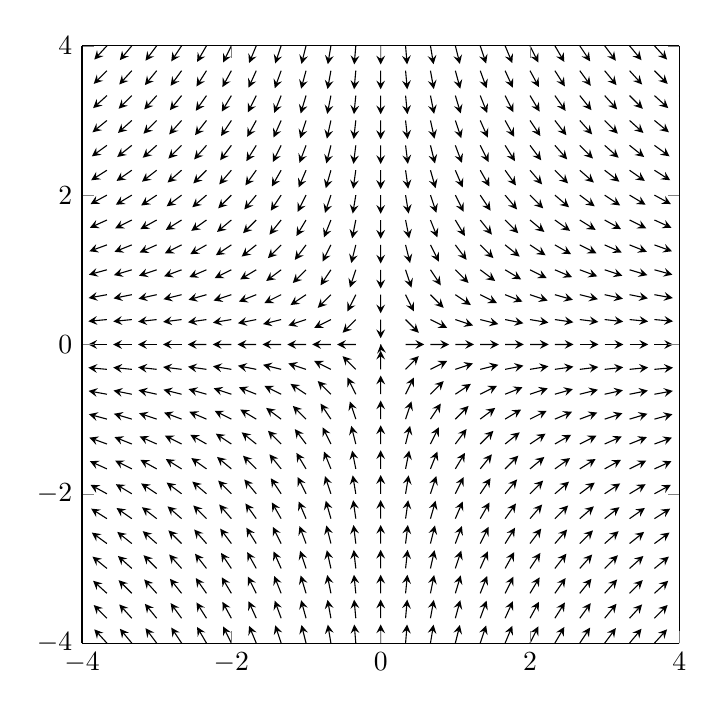
\begin{tikzpicture}
        \begin{axis}[
            xmin = -4, xmax = 4,
            ymin = -4, ymax = 4,
            zmin = 0, zmax = 1,
            axis equal image,
            xtick distance = 2,
            ytick distance = 2,
            view = {0}{90},
            scale = 1.4,
            height=7cm,
            %xlabel = {$x$},
            %ylabel = {$y$}
        ]
            \addplot3[
                point meta = {sqrt(x^2+y^2)},
                quiver = {
                    u = {x/sqrt(x^2+y^2+0.0001)},
                    v = {-y/sqrt(x^2+y^2+0.000001)},
                    scale arrows = 0.25,
                },
                %quiver/colored = {mapped color},
                -stealth,
                domain = -4:4,
                domain y = -4:4,
            ] {0};
        \end{axis}
    \end{tikzpicture}\\
%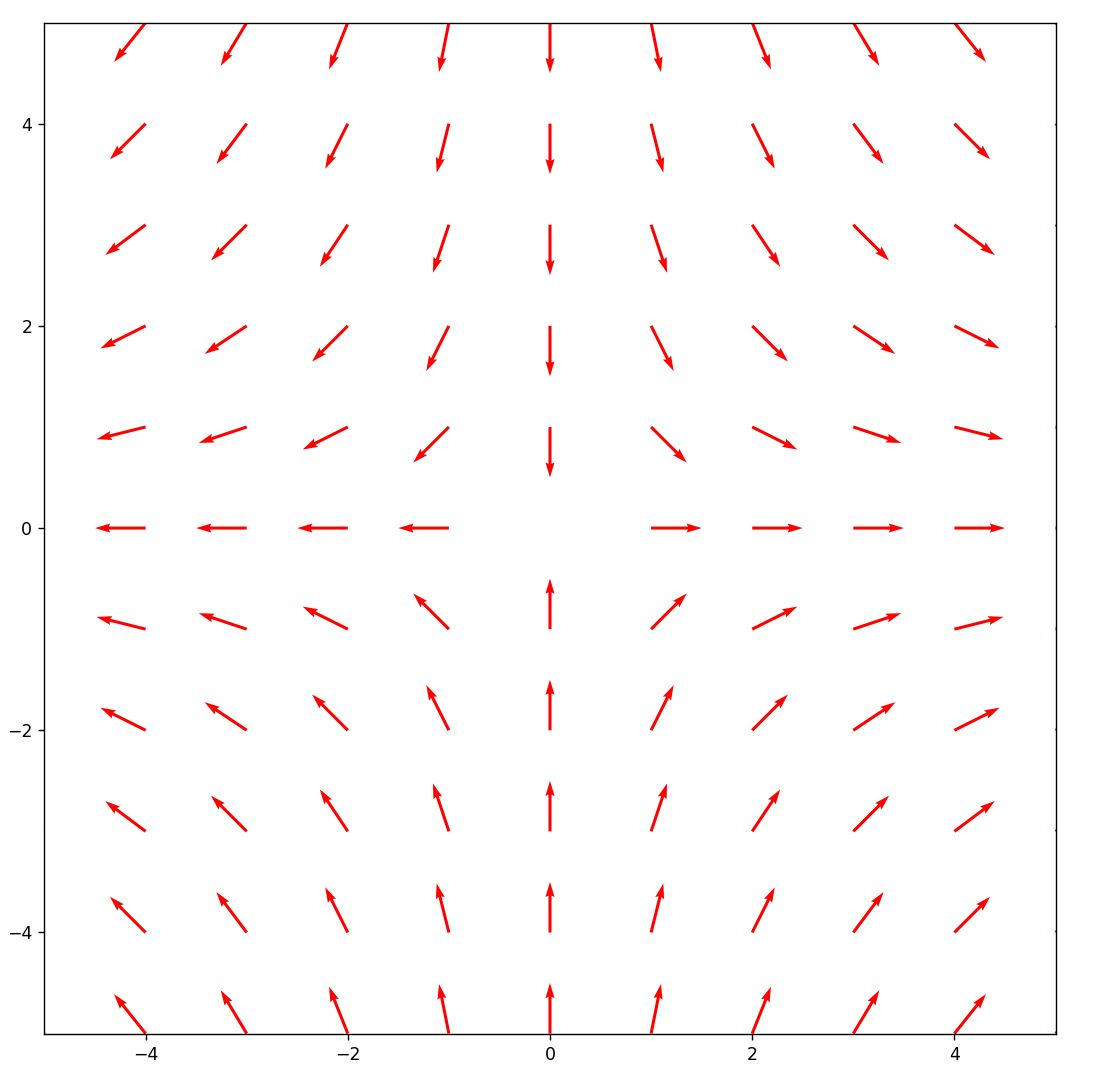
\includegraphics[scale=.3]{unitvectorfield1.jpg}
\end{minipage}\hfill
\begin{minipage}[H]{0.4\textwidth}
%\centering
\vspace{50pt}
$$V:\mathbb{R}_*^2\rightarrow \mathbb{R}^2|V(x,y) = \left< \frac{x}{\sqrt{x^2+y^2}},-\frac{y}{\sqrt{x^2+y^2}} \right>$$
\end{minipage}
\caption{Vector field for which $\lambda^r_{|s}\lambda_s = 0$ does not hold}
\label{fig:fig_p62_236_a}
\end{figure}
Put $ r = \sqrt{x^2+y^2}$, we get (as we have a Cartesian Coordinate system, the  Christoffel symbols vanish and the covariant components of the vectors are equal to their contravariant part):
\newpage
\begin{align}
\ & \left \{ \begin{array}{c}
\ V^1 = V_1 = +\frac{x}{r}\\
\ V^2 = V_2 = -\frac{y}{r}\\
\end{array}\right.\\
\ & \left \{ \begin{array}{cc}
\ V^1_{\ |1} =  V_{1|1} = \frac{y^2}{r^3}&V^1_{\ |2} =  V_{1|2} = -\frac{xy}{r^3}\\A
\ V^2_{\ |1} =  V_{2|1} = \frac{xy}{r^3}&V^2_{\ |2} =  V_{2|2} = -\frac{x^2}{r^3}\\
\end{array}\right.\\
\Rightarrow \quad\quad &\left \{ \begin{array}{c} \  V^1_{\ |s}V_s = V^1_{\ |1}V_1+V^1_{\ |2}V_2 = \frac{y^2}{r^3}\frac{x}{r}+ (-\frac{xy}{r^3})(-\frac{y}{r}) = \frac{xy^2}{r^4} \ne 0\\
\ V^2_{\ |s}V_s = V^2_{\ |1}V_1+V^2_{\ |2}V_2 = \frac{xy}{r^3}\frac{x}{r}+ (-\frac{y}{r})(-\frac{y}{r}) = \frac{x^2 y}{r^4} \ne 0
\end{array} \right.
\end{align}
Just as a check, we calculate $V^r_{|s}V_r$ which should be zero:
\begin{align}
\Rightarrow \quad\quad &\left \{ \begin{array}{c}V^s_{\ |1}V_s = V^1_{\ |1}V_1+V^2_{\ |1}V_2 = (+\frac{y^2}{r^3})\frac{x}{r}+ (+\frac{xy}{r^3})(-\frac{y}{r}) =0\\
\ V^s_{\ |2}V_s = V^1_{\ |2}V_1+V^2_{\ |2}V_2 = (-\frac{xy}{r^3})\frac{x}{r}+ (-\frac{y}{r})(-\frac{x^2}{r^3}) = 0
\end{array} \right.
\end{align}\\\\
Now, let's consider another unit vector field in a Cartesian Coordinate system:
\begin{figure}[H]

\centering
\begin{minipage}[H]{.4\textwidth}
%\centering
\vspace{0pt}
%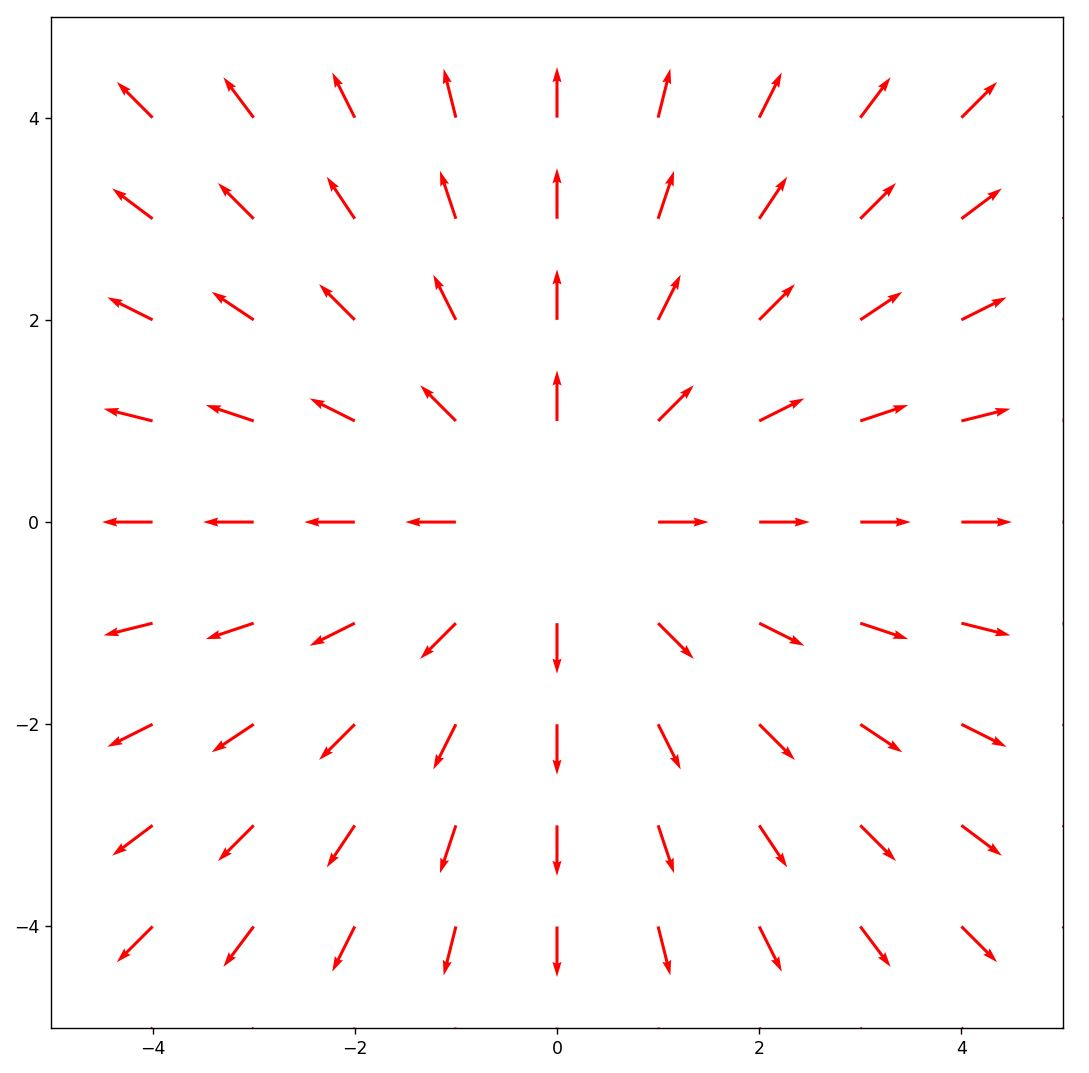
\includegraphics[scale=.3]{unitvectorfield2.jpg}
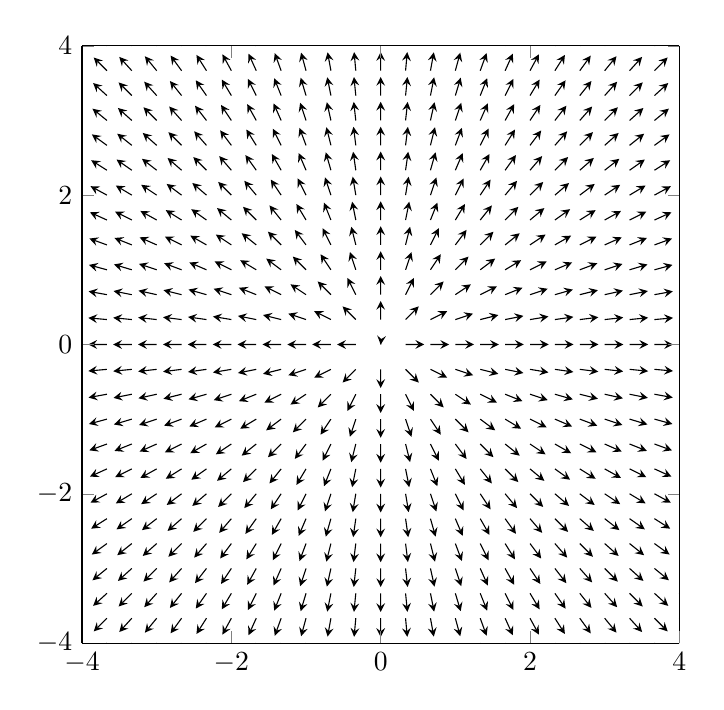
\begin{tikzpicture}
        \begin{axis}[
            xmin = -4, xmax = 4,
            ymin = -4, ymax = 4,
            zmin = 0, zmax = 1,
            axis equal image,
            xtick distance = 2,
            ytick distance = 2,
            view = {0}{90},
            scale = 1.4,
            height=7cm,
            %xlabel = {$x$},
            %ylabel = {$y$}
        ]
            \addplot3[
                point meta = {sqrt(x^2+y^2)},
                quiver = {
                    u = {x/sqrt(x^2+y^2+0.0001)},
                    v = {y/sqrt(x^2+y^2+0.000001)},
                    scale arrows = 0.25,
                },
                %quiver/colored = {mapped color},
                -stealth,
                domain = -4:4,
                domain y = -4:4,
            ] {0};
        \end{axis}
    \end{tikzpicture}\\
\end{minipage}\hfill
\begin{minipage}[H]{0.4\textwidth}
%\centering
\vspace{50pt}
$$V:\mathbb{R}_*^2\rightarrow \mathbb{R}^2|V(x,y) = \left< \frac{x}{\sqrt{x^2+y^2}},\frac{y}{\sqrt{x^2+y^2}} \right>$$
\end{minipage}
\caption{Vector field for which $\lambda^r_{|s}\lambda_s = 0$ hold}
\label{fig:fig_p62_236_b}
\end{figure}
\begin{align}
\ & \left \{ \begin{array}{c}
\ V^1 = V_1 = +\frac{x}{r}\\
\ V^2 = V_2 = +\frac{y}{r}\\
\end{array}\right.\\
\ & \left \{ \begin{array}{cc}
\ V^1_{\ |1} =  V_{1|1} = \frac{y^2}{r^3}&V^1_{\ |2} =  V_{1|2} = -\frac{xy}{r^3}\\
\ V^2_{\ |1} =  V_{2|1} = -\frac{xy}{r^3}&V^2_{\ |2} =  V_{2|2} = +\frac{x^2}{r^3}\\
\end{array}\right.\\
\Rightarrow \quad\quad &\left \{ \begin{array}{c} \  V^1_{\ |s}V_s = V^1_{\ |1}V_1+V^1_{\ |2}V_2 = (+\frac{y^2}{r^3})\frac{x}{r}+ (-\frac{xy}{r^3})(+\frac{y}{r}) =  0\\
\ V^2_{\ |s}V_s = V^2_{\ |1}V_1+V^2_{\ |2}V_2 = (-\frac{xy}{r^3})\frac{x}{r}+ (+\frac{y}{r})(+\frac{y}{r}) =  0
\end{array} \right.
\end{align}
Just as a check, we calculate $V^r_{|s}V_r$ which should be zero:
\begin{align}
\Rightarrow \quad\quad &\left \{ \begin{array}{c}V^s_{\ |1}V_s = V^1_{\ |1}V_1+V^2_{\ |1}V_2 = (+\frac{y^2}{r^3})(+\frac{x}{r})+ (-\frac{xy}{r^3})(+\frac{y}{r}) =0\\
\ V^s_{\ |2}V_s = V^1_{\ |2}V_1+V^2_{\ |2}V_2 = (-\frac{xy}{r^3})(+\frac{x}{r})+ (+\frac{y}{r})+\frac{x^2}{r^3}) = 0
\end{array} \right.
\end{align}\\
So, in the second example the relationship $\lambda^r_{|s}\lambda_s = 0$ holds.
Question (to investigate further and later) : does the fact that in the first case $\grad \maal \overline{V}  \ne 0$ and in the second case $\grad \maal \overline{V}= 0$, means that there is some relation with this expression?
$$\blacklozenge$$
\newpage

\section{p64-clarification 2.625}
\begin{tcolorbox}
$\textbf{2.625} \quad\quad\quad\quad\quad\quad \dv{ x^r}{x^N} = \frac{X^r}{X^N}$
\end{tcolorbox}
Be $C$ a surface defined by the function $F(x^1,\dots, x^{N-1}) = C$ and  $c_{\perp}$ the curve intersecting the surface $C$ perpendicularly at a point $p$.\\
Along the curve at that point $p$ we have
\begin{align}
\text{as}\quad\quad & \left \{ \begin{array}{cc}
\dv{ x^r}{s}& \text{is the tangent vector along}\quad c_{\perp}\\
\ X^r = a^{rn}\pdv{F}{x^n}& \text{ is orthogonal on the surface (2.623)}\quad C\\
\end{array}\right.\\
\Rightarrow \quad\quad & \dv{ x^r}{s} = kX^r
\end{align}
So, $\dv{ x^r}{s}$ is proportional to $X^r$ (as the curve intersects the surface orthogonally). This means that also all the components (coordinates) of both quantities are proportional. And so,
\begin{align}
\frac{\dv{ x^r}{s}}{\dv{ x^N}{s}} &= \frac{kX^r}{kX^N}\\
\Rightarrow\quad\quad \dv{ x^r}{x^N} &= \frac{X^r}{X^N}
\end{align}
$$\blacklozenge$$
\newpage

\section{p65-exercise}
\begin{tcolorbox}
Deduce from $\textbf{2.629}$ that $$a^{N \rho} = 0  \quad\quad a^{NN} = \frac{1}{a_{NN}}$$
\end{tcolorbox}
We have (see 2.629):
\begin{align}
\ a_{N\rho} =0\\
\text{and also}\quad\quad a_{Nm}a^{ms} = \delta^s_N
\end{align}
In (2) split the $m$ index in the subspace and the remaining coordinate $N$
\begin{align}
\ a_{N\rho}a^{\rho s} +  a_{NN}a^{N s} &= \delta^s_N\\
\text{as}\quad a_{N\rho} =0 \Rightarrow \quad\quad a_{NN}a^{N s} &= \delta^s_N
\end{align}\\
Case 1: $s\ne N$
\begin{align}
\  a_{NN}a^{N s} =0 \quad \Leftrightarrow \quad a_{NN}a^{N \rho} =0 \quad\quad \text{(as}\quad s\ne N \text{)}\\
\text{as we suppose}\quad a_{NN}\ne 0 \quad \Rightarrow \quad a^{N \rho} =0
\end{align}\\

Case 2: $s= N$
\begin{align}
\  a_{NN}a^{N N} &=1 \\
\Rightarrow \quad a^{N N} &=\frac{1}{a_{NN}}
\end{align}
$$\blacklozenge$$
\newpage


\section{p69-clarification on 2.645}
\begin{tcolorbox}
In 2.645 we have $$T_{\alpha | \beta} =T_{\alpha || \beta}  +\frac{1}{2}\frac{1}{a_{NN}}\partial_N  a_{\alpha\beta}T_{N}$$ and $$T_{\alpha | \beta} =T_{\alpha || \beta}  +\frac{1}{2}\partial_N  a_{\alpha\beta}T^{N}$$
\end{tcolorbox}
Indeed,
\begin{align}
\ T^N &= a^{mN}T_m\\
\ & = a^{\alpha N}T_{\alpha}+a^{N N}T_{N}\\
\text{but (2.631)}\quad\quad a^{\alpha N} &= 0\\
\Rightarrow \quad\quad T^N &= a^{NN} T_N\\
\text{as}\quad a^{NN}= \frac{1}{a_{NN}} \quad \Rightarrow \quad\quad  T_{\alpha | \beta} &= T_{\alpha || \beta}  + \frac{1}{2}\partial_N  a_{\alpha\beta}T^{N}
\end{align}
$$\blacklozenge$$
\newpage
\section{p69-exercise}
\begin{tcolorbox}
Show that
$$\textbf{2.648}\quad\quad T^{\alpha}_{\ |\beta} = T^{\alpha}_{\ ||\beta} + \half a^{\alpha \mu} \partial_N a_{\mu\beta}T^N$$
$$\textbf{2.649}\quad\quad T^{N}_{\ |\alpha} = \partial_{\alpha}T^{N} - \frac{1}{2 a_{NN}} \partial_N a_{\alpha\mu}T^{\mu} + \frac{1}{2 a_{NN}} \partial_{\alpha} a_{NN}T^{N}$$
$$\textbf{2.650}\quad\quad T^{\alpha}_{\ |N} = \partial_{N}T^{\alpha}  + \half a^{\alpha\mu} \partial_N a_{\mu\sigma}T^{\sigma} - \half a^{\alpha\mu}  \partial_{\mu} a_{NN}T^{N}$$
\end{tcolorbox}
i) $T^{\alpha}_{\ |\beta} = T^{\alpha}_{\ ||\beta} + \half a^{\alpha \mu} \partial_N a_{\mu\beta}T^N$\\
\begin{align}
\textbf{(2.520)}\quad\quad \Rightarrow \quad\quad T^{\alpha}_{\ |\beta} &= \partial_{\beta}T^{\alpha}+\Gamma^{\alpha}_{m\beta}T^m \quad\quad\text{(}m = 1,\dots,N \text{)}\\
\Leftrightarrow \quad\quad T^{\alpha}_{\ |\beta} &= \underbrace{ \partial_{\beta}T^{\alpha}+ \Gamma^{\alpha}_{\mu \beta} T^{\mu}}_{T^{\alpha}_{ \ || \beta}} +\Gamma^{\alpha}_{N \beta}T^{N}\\
\textbf{(2.639)}\quad\quad \Gamma^{\alpha}_{N\beta} &= \half a^{\alpha \mu}\partial_N a^{\mu \beta}\\
\text{(2) and (3): }\quad\quad T^{\alpha}_{\ |\beta} &= T^{\alpha}_{\ ||\beta} + \half a^{\alpha \mu} \partial_N a_{\mu\beta}T^N
\end{align}
$$\diamond$$
Remark: We also use $\textbf{(2.639)}$ for the two other identities.\\\\
ii) $T^{N}_{\ |\alpha} = \partial_{\alpha}T^{N} - \frac{1}{2 a_{NN}} \partial_N a_{\alpha\mu}T^{\mu} + \frac{1}{2 a_{NN}} \partial_{\alpha} a_{NN}T^{N}$\\
\begin{align}
\textbf{(2.520)}\quad\quad \Rightarrow \quad\quad T^{N}_{\ |\alpha} &= \partial_{\alpha}T^{N}+\Gamma^{N}_{m\alpha}T^m \quad\quad\text{(}m = 1,\dots,N \text{)}\\
\Leftrightarrow \quad\quad T^{N}_{\ |\alpha} &=  \partial_{\beta}T^{\alpha}+ \underbrace{\Gamma^{N}_{\sigma \alpha}}_{ - \frac{1}{2a_{NN}}\partial_N a_{\sigma\alpha}} T^{\sigma } +\underbrace{\Gamma^{N}_{N \alpha}}_{ \frac{1}{2a_{NN}}\partial_{\alpha} a_{NN}}T^{N}\\
\Rightarrow \quad\quad T^{N}_{\ |\alpha} &=  \partial_{\beta}T^{\alpha} - \frac{1}{2a_{NN}}\partial_N a_{\sigma\alpha}T^{\sigma } +\frac{1}{2a_{NN}}\partial_{\alpha} a_{NN}T^{N}
\end{align}\\
iii) $T^{\alpha}_{\ |N} = \partial_{N}T^{\alpha}  + \half a^{\alpha\mu} \partial_N a_{\mu\sigma}T^{\sigma} - \half a^{\alpha\mu}  \partial_{\mu} a_{NN}T^{N}$\\
\begin{align}
\textbf{(2.520)}\quad\quad \Rightarrow \quad\quad T^{\alpha}_{\ |N} &= \partial_{N}T^{\alpha}+\Gamma^{\alpha}_{mN}T^m \quad\quad\text{(}m = 1,\dots,N \text{)}\\
\Leftrightarrow \quad\quad T^{\alpha}_{\ |N} &=  \partial_{N}T^{\alpha}+ \underbrace{\Gamma^{\alpha}_{\sigma N }}_{ \half a^{\alpha \mu}\partial_N a_{\mu\sigma}}  T^{\sigma }+\underbrace{\Gamma^{\alpha}_{N N}}_{ -\half a^{\alpha\mu}\partial_{\mu} a_{NN}}T^{N}\\
\Rightarrow \quad\quad T^{\alpha}_{\ |N} &=  \partial_{N}T^{\alpha}+ \half a^{\alpha \mu}\partial_N a_{\mu\sigma}T^{\sigma } -\half a^{\alpha\mu}\partial_{\mu} a_{NN}T^{N}
\end{align}
$$\blacklozenge$$
\newpage

\section{p71-exercise}
\begin{tcolorbox}
Write down equation 2.643 tot 2.650 for the special cae of a geodesic normal coordinate system.
\end{tcolorbox}
\begin{align}
\ \textbf{(2.643)}\quad \quad T_{\alpha || \beta} &= \partial_{\beta}T_{\alpha} - \Gamma^{\gamma}_{\alpha\beta}T_{\gamma}\quad\quad \text{(does not change)}\\
\textbf{(2.644)}\quad \quad T_{\alpha | \beta} &=T_{\alpha || \beta}  - \underbrace{\Gamma^{N}_{\alpha\beta}}_{=\frac{1}{2} \frac{1}{a_{NN}}\partial_N  a_{\alpha\beta}}T_{N}\\
&=T_{\alpha || \beta}  +\frac{1}{2} \epsilon\partial_N  a_{\alpha\beta}T_{N}\\
\textbf{(2.645)}\quad \quad T_{\alpha | \beta} &=T_{\alpha || \beta}  +\frac{1}{2}\partial_N  a_{\alpha\beta}T^{N}\quad\quad \text{(does not change)}\\
\textbf{(2.646)}\quad \quad T_{N| \alpha } &=\partial_{\alpha}T_N  -\frac{1}{2}\partial_N  a_{\mu\alpha}T^{\mu} -\frac{1}{2}\underbrace{\partial_{\alpha}  a_{NN}}_{=0}T^{N}\\
&=\partial_{\alpha}T_N  -\frac{1}{2}\partial_N  a_{\mu\alpha}T^{\mu} \\
\textbf{(2.647)}\quad \quad T_{ \alpha |N } &=\partial_N T_{\alpha}  -\frac{1}{2}\partial_N  a_{\mu\alpha}T^{\mu} -\frac{1}{2}\underbrace{\partial_{\alpha}  a_{NN}}_{=0}T^{N}\\
&=\partial_N T_{\alpha}  -\frac{1}{2}\partial_N  a_{\mu\alpha}T^{\mu} \\
\textbf{(2.648)}\quad \quad T^{\alpha}_{ \  | \beta} &=T^{\alpha}_{ || \beta}  + \frac{1}{2}a^{\alpha\mu}\partial_N  a_{\mu\beta}T_{N}\quad\quad\text{(does not change)}\\
\textbf{(2.649)}\quad \quad T^N_{ \ | \alpha} &=\partial_{\alpha}T^N  -\frac{1}{2}\frac{1}{a_{NN}}\partial_N  a_{\mu\alpha}T^{\mu} -\frac{1}{2}\frac{1}{a_{NN}}\underbrace{\partial_{\alpha}  a_{NN}}_{=0}T^{N}\\
\ &= \partial_{\alpha}T^N  -\frac{1}{2}\epsilon\partial_N  a_{\mu\alpha}T^{\mu} \\
\textbf{(2.650)}\quad \quad T^{\alpha}_{\ |N} &=\partial_N T^{\alpha}  +\frac{1}{2}a^ {\alpha\mu}\partial_N  a_{\mu\sigma}T^{\sigma} -\frac{1}{2}a^{\alpha\mu}\underbrace{\partial_{\mu}  a_{NN}}_{=0}T^{N}\\
\ &=\partial_N T^{\alpha}  +\frac{1}{2}a^ {\alpha\mu}\partial_N  a_{\mu\sigma}T^{\sigma} 
\end{align}
\\\\
To investigate: note (3) and (4) which suggest that $\epsilon T_{N} = T^{N}$. Prove formally?
$$\blacklozenge$$
\newpage


\section{p73-Clarification 2.706}
\begin{tcolorbox}
... Let us now define a unit vector $\lambda^r_{(2)}$ and a positive invariant $\kappa_{(2)}$ by the equation \\
\begin{align}
\left \{ \begin{array}{c}
\frac{\delta\lambda_{(1)}^r}{\delta s} = \kappa_{(2)}\lambda^r_{(2)} - \epsilon\epsilon_{(1)}\kappa_{(1)}\lambda^r\\
\epsilon_{(2)}\lambda^n_{(2)}\lambda_{(2)n} = 1
\end{array} \right.
\end{align}  
\end{tcolorbox}
We can state that $\kappa_{(2)}$ is an invariant but one has to check whether the expression $(1)$ implies that $\kappa_{(2)}$ is indeed invariant.\\
What we know is that $\lambda^r, \frac{\delta \lambda^r}{\delta s},\frac{\delta\lambda_{(1)}^r}{\delta s},  \lambda^r_{(2)}$ are contravariant vectors. Also $\kappa_{(1)}$ is an invariant as $\frac{\delta\lambda^r}{\delta s} = \kappa_{(1)}\lambda^r_{(1)}$ and the magnitude of $\frac{\delta\lambda^r}{\delta s}$ does not depend on the coordinate system. So,
\begin{align}
\text{(1)}\times \lambda_{(2)r} \quad\Rightarrow \quad\quad \frac{\delta\lambda_{(1)}^r}{\delta s}\lambda_{(2)r} &= \kappa_{(2)}\lambda^r_{(2)}\lambda_{(2)r} - \epsilon\epsilon_{(1)}\kappa_{(1)}\lambda^r\lambda_{(2)r}\\
\Rightarrow \quad\quad \kappa_{(2)}\underbrace{\lambda^r_{(2)}\lambda_{(2)r}}_{\text{invariant}} &= \underbrace{\frac{\delta\lambda_{(1)}^r}{\delta s}\lambda_{(2)r}}_{\text{invariant}}  + \underbrace{\epsilon\epsilon_{(1)}}_{\text{invariant}} \underbrace{\kappa_{(1)}}_{\text{invariant}} \underbrace{\lambda^r \lambda_{(2)r}}_{\text{invariant}} \\
\Rightarrow \quad\quad \kappa_{(2)}&= \text{invariant} 
\end{align}
$$\blacklozenge$$
\newpage

\section{p74-Clarification 2.710}
\begin{tcolorbox}
\begin{align}
\textbf{2.710}\quad\quad\left \{ \begin{array}{c}
\frac{\delta\lambda_{(M-1)}^r}{\delta s} = \kappa_{(M)}\lambda^r_{(M)} - \epsilon_{(M-2)}\epsilon_{(M-1)}\kappa_{(M-1)}\lambda^r_{(M-2)}\\
\epsilon_{(M-1)}\lambda^n_{(M-1)}\lambda_{(M-1)n} = 1\quad\quad \text{(M=1,2,...,N)}
\end{array} \right.
\end{align}
... It is easily proved by mathematical induction that the whole sequence of vectors defined by 2.710 are perpendicular to the tangent and to one another ...
\end{tcolorbox}
We already know from 2.703 to 2.709 that $\lambda^r, \lambda_{(1)}^r,\lambda_{(2)}^r,\lambda_{(3)}^r$, satisfying equations (1), are all mutually perpendicular. Let us assume that the orthogonality for the set $\{\lambda_{(k)}^r:k= 0,1,2,3,..., M-1\}$ has been verified. We prove by induction that then, $\lambda_{(M)}^r$ will be orthogonal to all elements of the set.\\
i) Consider the set $\{\lambda_{(k)}^r:k= 0,1,2,3,..., M-3\}$ where we already know that $\lambda_{(k)}^r$ are mutually perpendicular and also $\lambda_{(k)}^r \perp \lambda_{(M-1)}^r $, $\lambda_{(k)}^r \perp \lambda_{(M-2)}^r$ and $\lambda_{(M-1)}^r \perp \lambda_{(M-1)}^r \quad \forall k$.
\begin{align}
\text{(1)}\times \lambda_{(k)r}\quad\Rightarrow\quad\quad \frac{\delta\lambda_{(M-1)}^r}{\delta s}\lambda_{(k)r} &= \kappa_{(M)}\lambda^r_{(M)}\lambda_{(k)r} - \epsilon_{(M-2)}\epsilon_{(M-1)}\kappa_{(M-1)}\underbrace{\lambda^r_{(M-2)}\lambda_{(k)r}}_{=0}\\
\text{We have}  \quad \quad\quad\quad\quad\lambda_{(k)r}\lambda^r_{(M-1)} &=0\\
\Rightarrow \quad \quad\quad\quad\quad\ \frac{\delta\lambda_{(k)r}\lambda_{(M-1)}^r}{\delta s} &= \lambda_{(M-1)}^r\frac{\delta\lambda_{(k)r}}{\delta s}+\lambda_{(k)r}\delta\frac{\lambda_{(M-1)}^r}{\delta s}=0\\
\Rightarrow \quad \quad\quad\quad\quad\ \lambda_{(k)r}\delta\frac{\lambda_{(M-1)}^r}{\delta s} &= - \lambda_{(M-1)}^r\frac{\delta\lambda_{(k)r}}{\delta s}\\
\text{We have}\quad \quad\quad\quad\quad\frac{\delta\lambda_{(k)r}}{\delta s} &= \kappa_{(k+1)}\lambda_{(k+1)r} - \epsilon_{(k)}\epsilon_{(k-1)}\kappa_{(k)}\lambda_{(k-1)r}\\
\text{(5) and (6)}\Rightarrow \quad \quad\quad\quad\quad\ \lambda_{(k)r}\delta\frac{\lambda_{(M-1)}^r}{\delta s} &= -\kappa_{(k+1)}\underbrace{\lambda_{(k+1)r} \lambda_{(M-1)}^r}_{=0} - \epsilon_{(k)}\epsilon_{(k-1)}\kappa_{(k)}\underbrace{\lambda_{(k-1)r}\lambda_{(M-1)}^r}_{=0}\\
\text{From (2)}\Rightarrow \quad \quad\quad\quad\quad\ \kappa_{(M)}\lambda^r_{(M)}\lambda_{(k)r}&=0\\
\Rightarrow \quad \quad\quad\quad\quad\ \lambda^r_{(M)}& \perp\lambda_{(k)r}\quad\quad \forall k= 0,1,2,3,..., M-3 
\end{align}\\\\
ii) Consider the case $k = M-1$\\\begin{align}
\text{(1)}\times \lambda_{(M-1)r}\quad \frac{\delta\lambda_{(M-1)}^r}{\delta s}\lambda_{(M-1)r} &= \kappa_{(M)}\lambda^r_{(M)}\lambda_{(M-1)r} - \epsilon_{(M-2)}\epsilon_{(M-1)}\kappa_{(M-1)}\underbrace{\lambda^r_{(M-2)}\lambda_{(M-1)r}}_{=0}\\
\text{from (2.530):}\quad\quad \frac{\delta\lambda_{(M-1)}^r}{\delta s}\lambda_{(M-1)r}  &= \half\underbrace{\frac{\delta\lambda_{(M-1)r}\lambda_{(M-1)}^r}{\delta s}}_{=0\text{ as }\lambda_{(M-1)r}\lambda_{(M-1)}^r =  \epsilon_{(M-1)}}\\
\Rightarrow \quad \quad\quad\quad\quad \kappa_{(M)}\lambda^r_{(M)}\lambda_{(M-1)r}&=0\\
\Rightarrow \quad \quad\quad\quad\quad \lambda_{(M-1)r} & \perp\lambda_{(M)r}
\end{align}

iii) Consider the case $k = M-2$\\\begin{align}
\text{(1)}\times \lambda_{(M-2)r}\quad \frac{\delta\lambda_{(M-1)}^r}{\delta s}\lambda_{(M-2)r} &= \kappa_{(M)}\lambda^r_{(M)}\lambda_{(M-2)r} - \epsilon_{(M-2)}\epsilon_{(M-1)}\kappa_{(M-1)}\underbrace{\lambda^r_{(M-2)}\lambda_{(M-2)r}}_{=\epsilon_{(M-2)}}\\
\Rightarrow \quad \quad\quad\quad\quad\frac{\delta\lambda_{(M-1)}^r}{\delta s}\lambda_{(M-2)r} &= \kappa_{(M)}\lambda^r_{(M)}\lambda_{(M-2)r} - \epsilon_{(M-1)}\kappa_{(M-1)}\underbrace{\epsilon_{(M-2)}\epsilon_{(M-2)}}_{=1}\\
\Rightarrow \quad \quad\quad\quad\quad\frac{\delta\lambda_{(M-1)}^r}{\delta s}\lambda_{(M-2)r} &= \kappa_{(M)}\lambda^r_{(M)}\lambda_{(M-2)r} - \epsilon_{(M-1)}\kappa_{(M-1)}\\
\text{We have}  \quad \quad\quad\quad\quad\lambda_{(M-1)}^r\lambda_{(M-2)r} &=0\\
\Rightarrow \quad \quad\quad\quad\quad\ \lambda_{(M-2)r}\frac{\delta\lambda_{(M-1)}^r}{\delta s} &= -\lambda_{(M-1)}^r\frac{\delta\lambda_{(M-2)r}}{\delta s}\\
\text{We have also }  \quad\frac{\delta\lambda_{(M-2)r}}{\delta s} &= \kappa_{(M-1)}\lambda_{(M-1)r} - \epsilon_{(M-3)}\epsilon_{(M-2)}\kappa_{(M-2)}\lambda_{(M-3)r}\\
\text{(19)}\times \lambda^r_{(M-1)} \text{ and (18): }  \lambda_{(M-2)r}\frac{\delta\lambda_{(M-1)}^r}{\delta s} &= -\kappa_{(M-1)}\underbrace{\lambda^r_{(M-1)}\lambda_{(M-1)r}}_{=\epsilon_{(M-1)}} - \epsilon_{(M-3)}\epsilon_{(M-2)}\kappa_{(M-2)}\underbrace{\lambda^r_{(M-3)}\lambda_{(M-1)r}}_{=0}\\
\Rightarrow \quad \quad\quad\quad\quad\ \lambda_{(M-2)r}\frac{\delta\lambda_{(M-1)}^r}{\delta s} &= -\kappa_{(M-1)}\epsilon_{(M-1)}\\
\text{(16) and (21):}\quad \quad\quad\quad\quad -\kappa_{(M-1)}\epsilon_{(M-1)} &= \kappa_{(M)}\lambda^r_{(M)}\lambda_{(M-2)r} - \epsilon_{(M-1)}\kappa_{(M-1)}\\
\Rightarrow \quad \quad\quad\quad\quad \kappa_{(M)}\lambda^r_{(M)}\lambda_{(M-2)r}&=0\\
\Rightarrow \quad \quad\quad\quad\quad \lambda_{(M-2)r}\perp\lambda_{(M)r}
\end{align}
With, i), ii), iii) all possible cases are covered which makes the proof complete.
$$\blacklozenge$$
\newpage

\section{p75-Clarification 2.714}
\begin{tcolorbox}
$\textbf{2.714} \quad \quad (\kappa_{(1)})^2 = \epsilon_{(1)} a_{mn} \frac{\delta \lambda^{m}}{\delta s} \frac{\delta \lambda^{n}}{\delta s}$,   $\quad \quad \epsilon_{(1)} = \pm 1$
\end{tcolorbox}
\begin{align}
\ \frac{\delta \lambda^{n}}{\delta s} &= \kappa_{(1)}\lambda_{(1)}^{n}\\
\text{(1)}\times \text{(1)}\quad\Rightarrow \quad\quad \frac{\delta \lambda^{m}}{\delta s}\frac{\delta \lambda^{n}}{\delta s} &= (\kappa_{(1)})^2 \lambda_{(1)}^{m}\lambda_{(1)}^{n}\\
\text{(2)}\times a_{mn} \Rightarrow\quad\quad a_{mn}\frac{\delta \lambda^{m}}{\delta s}\frac{\delta \lambda^{n}}{\delta s} &= a_{mn}(\kappa_{(1)})^2 \lambda_{(1)}^{m}\lambda_{(1)}^{n}\\
\ &= (\kappa_{(1)})^2 \underbrace{\lambda_{(1)m} \lambda_{(1)}^{n}}_{=\epsilon_{(1)}}\\
\ &= (\kappa_{(1)})^2 
\end{align}
$$\blacklozenge$$
\newpage


\section{p75-exercise}
\begin{tcolorbox}
For positive definite metric forms, write out explicitly the Frenet formulae for the case N=2, 3 and 4.
\end{tcolorbox}
The general Frenet formulae are 
\begin{align}
\left \{ \begin{array}{c}
\frac{\delta\lambda_{(M-1)}^r}{\delta s} = \kappa_{(M)}\lambda^r_{(M)} - \epsilon_{(M-2)}\epsilon_{(M-1)}\kappa_{(M-1)}\lambda^r_{(M-2)}\\
\epsilon_{(M-1)}\lambda^n_{(M-1)}\lambda_{(M-1)n} = 1\quad\quad \text{(M=1,2,...,N)}
\end{array} \right.
\end{align}
As $\Phi$ is positive definite, we have $\epsilon_{(k)} = 1\quad \forall k$
\begin{center}
\begin{tabular}{ |c|c|c|c| } 
\hline
N=2 & N=3 & N=4 \\
\hline
& &\\
$\frac{\delta\lambda^r}{\delta s} = \kappa_{(1)}\lambda^r_{(1)} $ & $\frac{\delta\lambda^r}{\delta s} = \kappa_{(1)}\lambda^r_{(1)} $& $\frac{\delta\lambda^r}{\delta s} = \kappa_{(1)}\lambda^r_{(1)} $ \\ 
$\frac{\delta\lambda_{(1)}^r}{\delta s} = \kappa_{(2)}\lambda^r_{(2)} - \kappa_{(1)}\lambda^r$& $\frac{\delta\lambda_{(1)}^r}{\delta s} = \kappa_{(2)}\lambda^r_{(2)} - \kappa_{(1)}\lambda^r$ & $\frac{\delta\lambda_{(1)}^r}{\delta s} = \kappa_{(2)}\lambda^r_{(2)} - \kappa_{(1)}\lambda^r$ \\ 
& $\frac{\delta\lambda_{(2)}^r}{\delta s} = \kappa_{(3)}\lambda^r_{(3)} - \kappa_{(2)}\lambda^r_{(1)}$ & $\frac{\delta\lambda_{(2)}^r}{\delta s} = \kappa_{(3)}\lambda^r_{(3)} - \kappa_{(2)}\lambda^r_{(1)}$ \\
& & $\frac{\delta\lambda_{(3)}^r}{\delta s} = \kappa_{(4)}\lambda^r_{(4)} - \kappa_{(3)}\lambda^r_{(2)}$ \\
$\lambda^n\lambda_n= 1$&$\lambda^n\lambda_n= 1$&$\lambda^n\lambda_n= 1$\\
$\lambda_{(1)}^n\lambda_{(1)n}= 1$&$\lambda_{(1)}^n\lambda_{(1)n}= 1$&$\lambda_{(1)}^n\lambda_{(1)n}= 1$\\
&$\lambda_{(2)}^n\lambda_{(2)n}= 1$&$\lambda_{(2)}^n\lambda_{(2)n}= 1$\\
&&$\lambda_{(3)}^n\lambda_{(3)n}= 1$\\
\hline
\end{tabular}
\end{center}
Taking into account that $\kappa_{(N)} = 0$ for a space $V_N$, we get,
\begin{center}
\begin{tabular}{ |c|c|c|c| } 
\hline
N=2 & N=3 & N=4 \\
\hline
& &\\
$\frac{\delta\lambda^r}{\delta s} = \kappa_{(1)}\lambda^r_{(1)} $ & $\frac{\delta\lambda^r}{\delta s} = \kappa_{(1)}\lambda^r_{(1)} $& $\frac{\delta\lambda^r}{\delta s} = \kappa_{(1)}\lambda^r_{(1)} $ \\ 
& &\\
$\frac{\delta\lambda_{(1)}^r}{\delta s} =  - \kappa_{(1)}\lambda^r$& $\frac{\delta\lambda_{(1)}^r}{\delta s} = \kappa_{(2)}\lambda^r_{(2)} - \kappa_{(1)}\lambda^r$ & $\frac{\delta\lambda_{(1)}^r}{\delta s} = \kappa_{(2)}\lambda^r_{(2)} - \kappa_{(1)}\lambda^r$ \\ 
& &\\
& $\frac{\delta\lambda_{(2)}^r}{\delta s} =  - \kappa_{(2)}\lambda^r_{(1)}$ & $\frac{\delta\lambda_{(2)}^r}{\delta s} = \kappa_{(3)}\lambda^r_{(3)} - \kappa_{(2)}\lambda^r_{(1)}$ \\
& &\\
& & $\frac{\delta\lambda_{(3)}^r}{\delta s} =  - \kappa_{(3)}\lambda^r_{(2)}$ \\
& &\\
$\lambda^n\lambda_n= 1$&$\lambda^n\lambda_n= 1$&$\lambda^n\lambda_n= 1$\\
& &\\
$\lambda_{(1)}^n\lambda_{(1)n}= 1$&$\lambda_{(1)}^n\lambda_{(1)n}= 1$&$\lambda_{(1)}^n\lambda_{(1)n}= 1$\\
& &\\
&$\lambda_{(2)}^n\lambda_{(2)n}= 1$&$\lambda_{(2)}^n\lambda_{(2)n}= 1$\\
& &\\
&&$\lambda_{(3)}^n\lambda_{(3)n}= 1$\\
& &\\
\hline
\end{tabular}
\end{center}
$$\blacklozenge$$
\newpage

\section{p76-exercise}
\begin{tcolorbox}
In an Euclidean space $V_N$, the fundamental form is given as $\Phi = dx^n dx^n$. Show that a curve which has $\kappa_{(2)} = 0$ and $\kappa_{(1)} = \text{constant}$ satisfies equations of the form
$$x^r = A^r\cos\kappa_{(1)}s + B^r\sin\kappa_{(1)}s + C^r$$ where $A^r, B^r, C^r$ are constants satisfying $$ A^rA^R = B^rB^r = \frac{1}{\kappa_{(1)}^2},\quad A^rB^r = 0$$
so that $A^r$ and $B^r$ are vectors of equal magnitude and perpendicular to one another. (This curve is a circle in the N-space)
\end{tcolorbox}
\begin{align}
\text{What we know}\quad\quad\quad\quad \Phi &= dx^n dx^n\\
\Rightarrow \quad\quad\quad\quad \left(a_{mn}\right) &= \left(\delta^m_n\right)\\
\text{and given } \spatie \kappa_{(1)} = \text{constant}& \quad \kappa_{(2)} = 0\quad \epsilon_{(1)}=\epsilon_{(2)}, \dots = 1\\
\text{we have (2.705) }\quad\quad\quad\quad \frac{\delta\lambda^r}{\delta s}&=  \kappa_{(1)} \frac{\delta\lambda_{(1)}^r}{\delta s} \quad \quad \text{with }\quad \lambda^r = \dv{x^r}{s}\\
\text{but}\quad\left(a_{mn}\right) = \left(\delta^m_n\right)\quad\Rightarrow\spatie \frac{\delta\lambda^r}{\delta s} &= \dv{\lambda^r}{s}\\
\text{(4) and (5)}\quad\Rightarrow\spatie \dv{\lambda^r}{s} &= \kappa_{(1)} \frac{\delta\lambda_{(1)}^r}{\delta s}\\
\text{also}\spatie \frac{\delta\lambda_{(1)}^r}{\delta s} &= \underbrace{\kappa_{(1)}}_{=0} \frac{\delta\lambda_{(1)}^r}{\delta s}-  \kappa_{(1)} \frac{\delta\lambda_{(1)}^r}{\delta s}
\end{align}
Hence we get the following set of equations
\begin{align}
\left \{ \begin{array}{c}
\dv{x^r}{s} = \lambda^r \\\\
\dv{\lambda^r}{s} = \kappa_{(1)} \lambda_{(1)}^r\\\\
\dv{\lambda_{(1)}^r}{ s} = -  \kappa_{(1)} \lambda_{(1)}^r\\\\
\kappa_{(1)} = \kappa\quad \text{(=constant)}\\\\
\kappa_{(2)} = 0\\\\
\lambda^n\lambda_n = 1\\\\
\lambda_{(1)}^n\lambda_{(1)n} = 1\\
\end{array} \right.\\
\text{(8)}\quad \Rightarrow \spatie \dv[2]{\lambda_{(1)}^r}{s} + \kappa ^2 \lambda_{(1)}^r = 0
\end{align}
Solving the ODE (9). Put $ e^{rs} = \lambda_{(1)}^k$
\begin{align}
\text{(9):}\spatie&  r^2 + \kappa^2 = 0\\
\Rightarrow \spatie & r = \pm \imath \kappa\\
\text{Hence, a general solution of (9) is of the form:} \spatie & \lambda_{(1)}^r = p^r e^{ \imath \kappa s}  + q^r e^{ -\imath \kappa s}\\
\text{put}\quad  p^r+q^r = A^{,r}\quad &\text{and}\quad p^r-q^r = B^{,r}\\
\Leftrightarrow \spatie p^r = \frac{A^{,r}+B^{,r}}{2} &\text{and}\quad p^r=\frac{A^{,r}-B^{,r}}{2}\\
\text{(12) can then be written as }\quad  \lambda_{(1)}^r = A^{,r}\frac{ e^{ \imath \kappa s}+  e^{ -\imath \kappa s}}{2} & + B^{,r}\frac{ e^{ \imath \kappa s}- e^{ -\imath \kappa s}}{2}\\
\text{or}\quad  \lambda_{(1)}^r = A^{,r}\cos \kappa s & + B^{,r}\sin \kappa s\\
\text{We have (8)}\spatie \spatie  \lambda^r =  & -  \kappa_{(1)} \dv{\lambda_{(1)}^r}{ s} \\
\dv{(16)}{s}\quad\text{and (17)}\Rightarrow\spatie \lambda^r =  A^{,r}\sin \kappa s & - B^{,r}\cos \kappa s\\
\text{as}\quad \lambda^r = \dv{x^r}{s}\quad\text{ with (18)}\quad \Rightarrow \spatie x^r = - \frac{A^{,r}}{\kappa}\cos \kappa s &  - \frac{B^{,r}}{\kappa}\sin \kappa s + C^r\\
\end{align}
Replace $- \frac{A^{,r}}{\kappa}$ with $A^{r}$ and $- \frac{B^{,r}}{\kappa}$ with $B^{r}$, we get then the following set of equations,

\begin{align}
\left \{ \begin{array}{c}
x^r = A^{r}\cos \kappa s   + B^{,r}\sin \kappa s + C^r\\
\lambda^r =  -\kappa A^{r}\sin \kappa s  +\kappa B^{r}\cos \kappa s\\
\lambda_{(1)}^r = - \kappa A^{r}\cos \kappa s  - \kappa B^{r}\sin \kappa s\\
\end{array} \right.\\
\text{with the following constraints}\spatie \lambda^n\lambda_n = 1\spatie 
\lambda_{(1)}^n\lambda_{(1)n} &= 1\\
\lambda^n\lambda_n = 1\quad\Rightarrow \kappa^2 A^r A^r \sin ^2 \kappa s+ \kappa^2 B^r B^r \cos ^2 \kappa s - 2 \kappa^2 A^rB^r\sin\kappa s\cos \kappa s &= 1\\
\text{or} \spatie A^r A^r \sin ^2 \kappa s+  B^r B^r \cos ^2 \kappa s - 2 A^rB^r\sin\kappa s\cos \kappa s &= \frac{1}{\kappa^2 }\\
\lambda_{(1)}^n\lambda_{(1)n} = 1\quad\Rightarrow \kappa^2 A^r A^r \cos ^2 \kappa s+ \kappa^2 B^r B^r \sin ^2 \kappa s + 2 \kappa^2 A^rB^r\sin\kappa s\cos \kappa s &= 1\\
\text{or} \spatie A^r A^r \cos ^2 \kappa s+  B^r B^r \sin ^2 \kappa s + 2 A^rB^r\sin\kappa s\cos \kappa s &= \frac{1}{\kappa^2 }\\
\text{Choose }\quad \kappa s = \frac{\pi}{2}\quad\text{and} \quad \kappa s = 0\\
\Rightarrow \spatie A^r A^r =  \frac{1}{\kappa^2 }\quad\text{and}\quad B^r B^r =  \frac{1}{\kappa^2 }\\
\text{Morover considering (26)-(24) and (28)}\quad \Rightarrow \spatie 2A^rB^r\sin \kappa s \cos \kappa s =0 \quad \forall \kappa s\\
\Rightarrow \spatie A^rB^r=0
\end{align}
Note: when deriving expressions $(23)$ and $(26)$ we use the fact that $\left(a_{mn}\right) =  \left(a^{mn}\right) = \left(\delta^m_n\right) $
$$\blacklozenge$$
\newpage

\section{p78-exercise 1}
\begin{tcolorbox}
For cylindrical coordinates in Euclidean 3-space, write down the metric form by inspection of a diagram showing a general infinitesimal displacement, and calculate all the Christoffel symbols of both kinds.
\end{tcolorbox}
\begin{figure}[h]

%\includegraphics[scale=.4]{polar3d.jpg}
\tdplotsetmaincoords{70}{120}
\begin{tikzpicture}
	[scale=9,
		tdplot_main_coords,
		axis/.style={->,black,thick},
		vector/.style={-stealth,black, thick},
		vector guide/.style={dashed,black,thick},
		angle/.style={black,thick}]

	%standard tikz coordinate definition using x, y, z coords
	
	\coordinate (O) at (0,0,0);
	\coordinate (P1) at (0.183,0.68297,0.34202);
	\coordinate (P) at (0.183,0.68297,0);
	
	%tikz-3dplot coordinate definition using r, theta, phi coords
	\tdplotsetcoord{S0}{1}{70}{45} 
	\tdplotsetcoord{S}{sin(70)}{90}{45}
	\tdplotsetcoord{S1}{sin(70)}{90}{75}
	\tdplotsetcoord{S2}{1}{70}{75} 
	\tdplotsetcoord{J}{1.1}{40}{75}
	\tdplotsetcoord{H}{1.1*cos(40)}{0}{0}
	\tdplotsetcoord{G}{1.*cos(70)}{0}{0}

	
	%labeling points
	\node[tdplot_main_coords,{anchor=south east}] at (O){$O$};
	\node[tdplot_main_coords,anchor=north  west] at (S){$S$};
	\node[tdplot_main_coords,anchor=north  west] at (S1){$S'$};
	\node[tdplot_main_coords,anchor=south west] at (S0){$S^0$};
	\node[tdplot_main_coords,anchor=north  west] at (S2){$S"$};
	
	\node[tdplot_main_coords,above,right] at (J){$J$};
	\node[tdplot_main_coords,{anchor=south east}] at (H){$H$};
	\node[tdplot_main_coords,{anchor=south east}] at (G){$G$};

	\node[tdplot_main_coords,{anchor=south west}] at (P1){$P'$};
	\node[tdplot_main_coords,{anchor=south west}] at (P){$P$};
	
	
	\foreach \v in {G,P1,P,H,S1,S2,S}  \draw[fill=gray] (\v) circle (0.2pt);
	
	%draw axes
	\draw[axis] (0,0,0) -- (1,0,0) node[anchor=north east]{$x$};
	\draw[axis] (0,0,0) -- (0,1,0) node[anchor=north west]{$y$};
	\draw[axis] (0,0,0) -- (0,0,1) node[anchor=south]{$z$};
	
	%draw a vector from O to P
	\draw[ vector, thick ] (O) -- (S0);
	\draw[vector,  thick] (O) -- (J)  ;
	
	%draw guiding lines
	\draw[dashed,tdplot_main_coords] (S2)-- (S1)  ;
	\draw[dashed,tdplot_main_coords] (J)-- (H)  ;
	\draw[dashed,tdplot_main_coords] (S2)-- (P1)  ;
	\draw[dashed,tdplot_main_coords] (P1)-- (G)  ;
	\draw[dashed,tdplot_main_coords] (S0)-- (G)  ;

	
	%draw guiding lines with labels to lines
	\draw [dashed,tdplot_main_coords](P1) --(J) node[midway,right] {$dz$};
	\draw [dashed,tdplot_main_coords](P) --(P1) node[midway,right] {$z$};
	\draw [dashed,tdplot_main_coords](S0) --(S) node[midway,right] {$z$};
	\draw [dashed,tdplot_main_coords](P) --(P1) node[midway,right] {$z$};
	\draw [dashed,tdplot_main_coords](O) --(S) node[midway,right] {$\quad r$};
	\draw [dashed,tdplot_main_coords](O) --(S1) node[midway,right] {$\quad r+dr$};

	
	%draw an arc illustrating the angle defining the orientation
	\tdplotdrawarc[angle,,-stealth]{(O)}{.25}{0}{45}{anchor=north}{$\theta$}
	\tdplotdrawarc[angle,,-stealth]{(O)}{.25}{45}{75}{anchor=north}{$d\theta$}
	
	\tdplotdrawarc[angle,,-stealth]{(G)}{.25}{45}{75}{anchor=north}{$d\theta$}
	%draw arc illustrating the rotation of first vector
	\tdplotdefinepoints(0,0,cos(70))(sin(70)*cos(45),sin(70)*sin(45),cos(70))(sin(70)*cos(75),sin(70)*sin(75),cos(70))
	\tdplotdrawpolytopearc[dashed,-{Stealth[length=3mm, width=3mm]}]{0.93969}{}{}%0.93969 = sin(70)
	\tdplotdefinepoints(0,0,0)(sin(70)*cos(45),sin(70)*sin(45),0)(sin(70)*cos(75),sin(70)*sin(75),0)
	\tdplotdrawpolytopearc[dashed,-{Stealth[length=3mm, width=3mm]}]{0.93969}{}{}%0.93969 = sin(70)


\end{tikzpicture}\\
\label{fig:fig_p78_247_a}
\end{figure}
From the figure we may (assuming an infinitesimal displacement), we may approximate $\left| \overrightarrow{SS^{,}} \right|$ with the arclength $r d\theta$ and assume $\left|  \overrightarrow{S°S^{,,}} \right| \perp \left|  \overrightarrow{GS^{,}} \right|$) Hence, the infinitesimal displacement from S
\begin{align}
\ ds^2 &= \left| \overrightarrow{SS^{,}} \right|^2 + \left| \overrightarrow{S^{,,}P^{,}} \right|^2+\left| \overrightarrow{P^{,}J} \right|^2\\
\ &= dr^2 + ((r+dr)d\theta)^2 + dz^2\\
\ &= dr^2 + r^2d\theta^2 + dz^2\\
\text{Hence} \spatie &\left(a_{mn}\right) = \begin{pmatrix}
 1& 0 & 0 \\
 0&  r^2&0  \\
 0&0  &1  \\
\end{pmatrix}\quad\text{and}\quad \left(a_{mn}\right) = \begin{pmatrix}
 1& 0 & 0 \\
 0&  ^\frac{1}{r^2}&0  \\
 0&0  &1  \\
\end{pmatrix}
\end{align}
Note that all $a_{mn} = 0 \quad \forall m\ne n$. So,
\begin{align}
\left \{ \begin{array}{c}
\ [r \ r,r]=[\theta \  \theta, \theta] = [z \ z,z] = 0\\
\ [r \ \theta,r]=[r \ r, \theta] = [r \ r,z] = 0\\
\ [r \ z,\theta]=[z \  \theta, r] = [z \ \theta,z] = 0\\
\end{array}\right.\\
\text{But:}\spatie [\theta \ \theta,r]= -r \quad\text{and}\quad [r \  \theta, \theta] = r\\
\text{Hence}\spatie \left \{ \begin{array}{c}
\Gamma^m_{nk} = 0 \quad\forall\quad (nk) \ne (r, \theta), (\theta, \theta)\\\\
\Gamma^{\theta}_{r\theta} = \frac{1}{r} \quad\text{and}\quad \Gamma^r_{\theta\theta} = -r
\end{array}\right.\
\end{align}

$$\blacklozenge$$
\newpage

\section{p78-exercise 2}
\begin{tcolorbox}
If $a_{rs}$ and $b_{rs}$ are covariant tensors, show that the roots of the determinant equation $$\left|Xa_{rs} - b_{rs}\right |= 0$$ are invariants.
\end{tcolorbox}
\begin{align}
\text{Be}\spatie c_{rs} &= Xa_{rs} - b_{rs}\\
\text{Given }\spatie a_{rs} &= a^{,}_{mk}\pdv{x^{,m}}{x^r} \pdv{x^{,k}}{x^s}\\
\text{and }\spatie b_{rs} &= b^{,}_{mk}\pdv{x^{,m}}{x^r} \pdv{x^{,k}}{x^s}\\
\text{(1) }\quad\Rightarrow\spatie c_{rs} &= \underbrace{(Xa^{,}_{mk}-b^{,}_{mk})}_{=c^{,}_{km}} \pdv{x^{,m}}{x^r} \pdv{x^{,k}}{x^s}\\
\ &= c^{,}_{km} \pdv{x^{,m}}{x^r} \pdv{x^{,k}}{x^s}\\
\text{Be}\spatie J &= \left |\pdv{x^{,m}}{x^r}\right |= \left |\pdv{x^{,k}}{x^s}\right |\\
\text{In (5) put  }\spatie d_{kr} &= c^{,}_{km} \pdv{x^{,m}}{x^r} \\
\Rightarrow\spatie c_{rs} &= d^{,}_{kr} \pdv{x^{,k}}{x^s}\\
\text{or in matrix form  } \spatie C &= D^T J\quad \text{with}\quad D = C^{,}J\\
\Rightarrow\spatie \left |C \right| &= \left | (C^{,}J)^T J\right |\\
\Leftrightarrow\spatie \left |C \right| &= \left | C^{,}\right | \left |J\right |\left |J\right |
\end{align}
As $ \left |J\right | \ne 0$ ( $J$ is the Jacobian of the transformation, and thus can't be zero), then $$\left |C \right| = 0 \Rightarrow \left |C^{,} \right| = 0$$.\\
So, the root of $\left |C \right| = 0 $ is also a root of $\left |C^{,} \right| = 0$ and is as a consequence, invariant.

$$\blacklozenge$$
\newpage

\section{p78-exercise 3}
\begin{tcolorbox}
Is the form $dx^2+3dxdy+4dy^2+dz^2$ positive definite?
\end{tcolorbox}
\begin{align}
\Phi &= dx^2+3dxdy+4dy^2+dz^2\\
\text{Put (1) in the form}\spatie  \Phi &= X^2+3XY+4Y^2+Z^2\\
\text{Z has only a positive contribution: so put }\quad Z=0\quad\Rightarrow \quad \Phi &= X^2+3XY+4Y^2\\
\text{(3) can only be zero or negative if }\quad XY < 0\quad\text{:put}\quad Y & =-aX\quad (a>0)\\
\Rightarrow \Phi &= X^2-3aX^2 +4a^2X^2\\
\text{The roots of (5) are }\quad a_{1,2} &= \frac{3\pm \sqrt{9-16}}{8}
\end{align}
So, by (6) we can't get a $a \in \mathbb{R}_*$, so that (1) can be $0$ or negative. Hence,
$$\text{The form}\quad \Phi \quad \text{is positive definite}$$
$$\blacklozenge$$
\newpage

\section{p78-exercise 4}
\begin{tcolorbox}
If $X^r, Y^r$ are unit vectors inclined at an angle $\theta$, prove that $$\sin^2 \theta = (a_{rm}a_{sn}- a_{rs}a_{mn})X^r Y^s X^m Y^n$$
\end{tcolorbox}
$X^r Y^s$ are unit vectors. So,
\begin{align}
\ a_{rm}X^rX^m = 1 \quad &\text{and}\quad a_{sn}Y^sY^n = 1\\
\text{We have}\spatie \sin^2\theta &= 1 - \cos^2\theta\\
\text{and (2.312)}\spatie \cos\theta &= a_{mn}X^mY^n\\
\Rightarrow\spatie \sin^2 \theta &= a_{rm}X^rX^m a_{sn}Y^sY^n - a_{mn}X^mY^na_{rs}X^rY^s\\
\ &= (a_{rm} a_{sn} - a_{mn}a_{rs})X^rY^sX^mY^n
\end{align}
$$\blacklozenge$$
\newpage

\section{p78-exercise 5}
\begin{tcolorbox}
Show that, if $\theta$ is the angle between the normals to the surfaces $x^1 = C^{st}, x^2 = C^{st}$, then $$ \cos \theta = \frac{a^{12}}{\sqrt{a^{11}a^{22}}}$$
\end{tcolorbox}
\begin{align}
\text{be}\spatie \phi^{,}_1(x^1,x^2,\dots,x^N) = C^{st} \quad \phi^{,}_2(x^1,x^2,\dots,x^N) = C^{st}
\end{align}
the two equations representing $S_1, S_2$ (see page 63). We can rewrite (1) as:
\begin{align}
\ x^1 &= \phi^{,}_1(x^1,x^2,\dots,x^N) = C^{st} \\
\ x^2 &= \phi^{,}_2(x^1,x^2,\dots,x^N) = C^{st}\\
\text{From (2.622) we know that}\quad X^m = a^{mn}\partial_n \phi_{1} & ,\ Y^m = a^{mn}\partial_n \phi_{2} \ \text{are}\perp\text{vectors to the surfaces}\  \phi_{1},\phi_{2}\\
\text{We know also} \spatie \left|X^m\right |^2 &= a^{mk}X^mX^k\\
\ & = a_{mk}a^{mn}\partial_n \phi_{1}a^{kp}\partial_p \phi_{1}\\
\ & = \delta^k_k a^{kp}\partial_n \phi_{1}\partial_p \phi_{1}\\
\ & = a^{np}\partial_n \phi_{1}\partial_p \phi_{1}\\
\text{as} \ \phi_1 = x^1 = C^{st} \ \Rightarrow \ &= a^{np}\delta^1_n \delta^1_p\\
\ &= \epsilon a^{11}\\
\text{Analog, we have}\spatie \left|Y^m\right |^2 &= \epsilon a^{22}\\
\text{By definition:}\spatie \cos\theta &= \frac{a_{mn}X^mY^n}{ \left|X^r\right | \left|Y^s\right |}\\
\text{and }\spatie a_{mn}X^mY^n &= a_{mn} a^{mk}\partial_k \phi_{1} \  a^{np}\partial_p \phi_{2}\\
\ &=\delta^k_n a^{np}\partial_k \phi_{1} \ \partial_p \phi_{2}\\
\ &=a^{kp}\partial_k \phi_{1} \ \partial_p \phi_{2}\\
\text{as} \ \phi_1 = x^1 = C^{st},  \ \phi_2 = x^2 = C^{st} \ \Rightarrow \ &= a^{kp}\delta^1_k\delta^2_p\\
\ &= a^{12}\\
\text{So (12) becomes with (10), (11) and (17)} \spatie \cos\theta &= \frac{a_{12}}{ \sqrt{\epsilon a^{11}\epsilon a^{22}}}\\
&= \frac{a_{12}}{ \sqrt{ a^{11} a^{22}}}
\end{align}
$$\blacklozenge$$
\newpage

\section{p78-exercise 6}
\begin{tcolorbox}
Let $x^1, \ x^2,\ x^3$ be rectangular Cartesian coordinates in Euclidean 3-space, and let $x^1, \ x^2$ be taken as coordinates on a surface $x^3 = f(x^1, \ x^2)$. Show that the Christoffel symbols of the second kind for the surface are $$ \Gamma^r_{mn} = \frac{f_r f_{mn}}{1+ f_n f_p}$$ the suffixes taking the values $1, \ 2$ and the subscripts indicating partial derivatives.
\end{tcolorbox}
We have (rectangular Cartesian coordinates in Euclidean 3-space)
\begin{align}
\ ds^2 &= (dx^1)^2 + (dx^2)^2+(dx^3)^2\\
\text{with} \spatie x^3 &= f(x^1, \ x^2)\\
\text{and thus } \spatie dx^3 &= \partial_1 f \ dx^1 + \partial_2 f \  dx^2\\
\Rightarrow \spatie ds^2 &= (1+ (\partial_1 f)^2) (dx^1)^2 + (1+ (\partial_2 f)^2) (dx^2)^2+ 2\partial_1 f \ \partial_2 f \ dx^1 dx^2\\
\text{put}\spatie & \left \{ \begin{array}{c}
\ f_1 = \partial_1 f\\
\ f_2 = \partial_2 f\\
\ f_{11} = \partial_{11} f\\
\ f_{22} = \partial_{22} f\\
\ f_{12} = f_{21 } = \partial_{12} f\\
\end{array}\right.\\
\text{from (4)}\spatie \left(a_{mn}\right) =& \begin{pmatrix}
 1+f_1 ^2& f_1f_2 \\
 f_1f_2& 1+f_2 ^2 \\
\end{pmatrix}\\
\Rightarrow\spatie \left|a_{mn}\right| &= (1+f_1 ^2)(1+f_2 ^2) - (f_1f_2)^2\\
\ & = 1 + f_1 ^2+f_2 ^2\\
\text{also} \spatie \left(a^{mn}\right) =& \frac{1}{1 + f_1 ^2+f_2 ^2}\begin{pmatrix}
 1+f_2 ^2& -f_1f_2 \\
 -f_1f_2& 1+f_1 ^2 \\
\end{pmatrix}
\end{align}
\begin{align}
\textbf{Calculating the Christoffels symbols:}\quad [mn,\ k] &= \half (\partial_m a_{nk}+\partial_n a_{mk}-\partial_k a_{mn})\\
\Rightarrow\spatie & \left \{ \begin{array}{c}
\ [11,\ 1] =  f_1 f_{11}\\
\ [11,\ 2] =  f_2 f_{11}\\
\ [12,\ 1] =  f_1 f_{12}\\
\ [12,\ 2] =  f_2 f_{21}\\
\ [22,\ 2] =  f_2 f_{22}\\
\end{array}\right.\\
\text{From (11) we can see that the general form is:}\quad [mn,s] &= f_{mn}f_s\\
\textbf{Calculating the Christoffels symbols:}\quad \Gamma^r_{mn} &= a_{rs}[mn,s]\\ 
\text{(13) with (12):}\quad \Gamma^r_{mn} &= a_{rs}f_{mn}f_s = f_{mn}(a^{rs}f_s)\\
\text{put } \Delta &= \frac{1}{1 + f_1 ^2+f_2 ^2}=\frac{1}{1 + f_p f_p} \\
\Rightarrow\spatie  \left \{ \begin{array}{ll}
\Gamma^1_{mn} & = (a_{11} f_1 + a_{12} f_2)f_{mn}\\
\ & =  \Delta(f_1  + f_2^2f_1 - f_1f_2^2)f_{mn}\\
\ & =  \Delta f_1 f_{mn}\\\\
\Gamma^2_{mn} & = (a_{21} f_1 + a_{22} f_2)f_{mn}\\
\ & =  \Delta(- f_1^2f_2+f_2   + f_2f_1^2)f_{mn}\\
\ & =  \Delta f_2 f_{mn}\\
\end{array}\right. & 
\end{align}
$$\Rightarrow\quad \Gamma^r_{mn} = \frac{f_r f_{mn}}{1 + f_p f_p}$$
$$\blacklozenge$$
\newpage

\section{p78-exercise 7}
\begin{tcolorbox}
Write down the differential equations of the geodesics on a sphere, using colatitude $\theta$ and the azimuth $\phi$ as coordinates. Integrate the differential equations and obtain a finite equation $$ A\sin \theta \cos \phi + B \sin \theta \sin \phi + C\cos\theta = 0$$
where $A,B,C$ are arbitrary constants.
\end{tcolorbox}
$$\textbf{We will use two different approaches to determine the relation and finally use a geometrical reasoning }$$ $$\textbf{allowing us to avoid solving the ODE's resulting from the above mentioned approaches.}$$\\
We will first find the solution, starting from the variational principle , defining a geodesic.
In spherical coordinates we have (see exercise page 27) $ds^2 = dr^2 +  r^2\sin^2(\theta)d\phi^2+ r^2d\theta^2$.\\
As $r=R= C^{st}$ this reduces to
\begin{align}
\ ds^2 = R^2\sin^2(\theta)d\phi^2+ R^2d\theta^2
\end{align}
So the length of a curve on the sphere from a point $P_1$ to another point $P_2$ , the curve being determined by $\theta = \theta(u)\quad \phi = \phi(u)$ is:\\
\begin{align}
\ L &= R\int_{P_1}^{P_2} = \sqrt{\sin^2(\theta)d\phi^2+ d\theta^2}du\\
\text{Be}\quad \theta &= u \quad \phi = \phi(\theta)\\
\Rightarrow \quad  L &= R\int_{\theta_1}^{\theta_2} = \sqrt{1+\sin^2(\theta)(\dv{\phi}{\theta})^2}d\theta
\end{align}
Applying the variational principle on L and using the Euler-Langrange equations:
\begin{align}
 \dv{\pdv{\mathcal{L}}{\dot{\phi}}}{\theta} - \pdv{\mathcal{L}}{\phi}&=0 \quad 
 \text{with}\quad \mathcal{L} = \sqrt{1+\sin^2(\theta)(\dot{\phi})^2}\\
 \text{as}\quad  \pdv{\mathcal{L}}{\phi}&=0\\
 \text{(5) becomes:} \quad \dv{\pdv{\mathcal{L}}{\dot{\phi}}}{\theta} &=0\\
 \Leftrightarrow \quad \pdv{\mathcal{L}}{\dot{\phi}} &= C\quad \ \text{(= constant)}\\
\text{with}\quad \pdv{\mathcal{L}}{\dot{\phi}} &= \pdv{\sqrt{1+\sin^2 \theta   \  \dot{\phi}^2 }}{\dot{\phi}}= \frac{\sin^2 \theta \  \dot{\phi}}{ \sqrt{1+\sin^2 \theta \ \dot{\phi}^2 }}\\
\text{(9) and (10):}\quad C^2 &= \frac{\sin^2 \theta \  \dot{\phi}}{ \sqrt{1+\sin^2 \theta \ \dot{\phi}^2 }} \\
\text{or}\quad \dot{\phi} &= \frac{C}{\sin \theta \sqrt{\sin^2 \theta - C^2}}
\end{align}
Solving the ODE (12). Put $u = \cot \theta \quad \Rightarrow \quad du = - \csc^2 d\theta = -\frac{1}{\sin^2\theta} d\theta$. So,  
\begin{align}
\phi &= -C\int \frac{\sin \theta}{ \sqrt{\sin^2 \theta - C^2}}du\\
&= -C\int \frac{du}{ \sqrt{1- \frac{C^2 }{\sin^2 \theta}}}\\
&= -C\int \frac{du}{ \sqrt{1- C^2 - C^2 \cot^2 \theta}}\\
&= -C\int \frac{du}{ \sqrt{1- C^2 - C^2 u^2}}\\
\text{be}\quad a&= \frac{\sqrt{1-C^2}}{C}\\
\text{(15) becomes}\quad \phi &= -\int \frac{1}{ \sqrt{a^2 -  u^2}}du\\
\text{put }\quad u &= av\\
\text{(18) becomes}\quad \phi &= -\int \frac{1}{ \sqrt{1 -  v^2}}dv\\
\ &= -\arccos v + C^{st}\\
\ &= -\arccos \frac{u}{a}  + \phi_0\\
\text{or:}\quad \frac{u}{a} &= \cos (\phi - \phi_0)  \ \text{(by choosing an adequate}\ \phi_0\text{)}\\
\text{so :}\quad \cot\theta &= a \cos (\phi - \phi_0)  \\
\text{expanding} \  \cos (\phi - \phi_0)\  \text{gives:} \quad  \frac{\cos\theta}{\sin\theta} &= \ A\cos\phi + B\sin\phi\\
\text{or:} \quad  A\cos\phi \sin\theta &+ B\sin\phi\sin\theta -\cos\theta=0
\end{align}
$$\diamond$$
\newpage
Finding the geodesics from the tensorial formula's.\\
Note: For ease of notation we put $R=1$ without losing any general solutions.

\begin{align}
\text{from (1) we get:}\quad (a_{mn}) &= \begin{pmatrix}
 1&  0\\
0 & \sin^2\theta \\
\end{pmatrix}\\
\text{and}\quad (a^{mn}) &= \begin{pmatrix}
 \frac{1}{\sin^2\theta}&  0\\
0 & 1 \\
\end{pmatrix}\\
\text{hence:}\quad & \left \{ \begin{array}{ll}
\Gamma^1_{11}  = 0&\Gamma^2_{11}  = 0\\
\Gamma^1_{12}  = 0&\Gamma^2_{12}  = \cot\theta\\
\Gamma^1_{22}  = -\cos\theta\sin\theta&\Gamma^2_{22}  = 0\\
\end{array}\right.
\end{align}
Finding the geodesics from the tensorial formula's, implies solving $2^{nd}$ order ODE's. In order to find the simpliest form to solve , we write down three possible forms of the geodesic equations:
\begin{align}
\text{arc-length s as independent variable}\quad& \left \{ \begin{array}{ll}
\ (a)&\dv[2]{\phi}{s} + 2 \cot\theta\dv{\phi}{s} \dv{\theta}{s} = 0\\\\
\ (b)&\dv[2]{\theta}{s} - \sin\theta\cos\theta(\dv{\phi}{s})^2  = 0\\\\
\ (c)&\ (\dv{\theta}{s})^2+\sin^2\theta(\dv{\phi}{s})^2 = 1\\\\
\end{array}\right.\\
\theta \text{ as independent variable}\quad& \left \{ \begin{array}{l}
\lambda =  - \sin\theta\cos\theta(\dv{\phi}{\theta})^2\\\\
\dv[2]{\phi}{\theta}  = \lambda \dv{\phi}{\theta}- 2 \cot\theta\dv{\phi}{\theta}  \\\\
\end{array}\right.\\
\Rightarrow \quad \dv[2]{\phi}{\theta}  &= - \sin\theta\cos\theta(\dv{\phi}{\theta})^3- 2 \cot\theta\dv{\phi}{\theta}  \\
\phi \text{ as independent variable}\quad& \left \{ \begin{array}{l}
\lambda =  2 \cot\theta\dv{\theta}{\phi}\\\\
\dv[2]{\theta}{\phi}  = \lambda \dv{\theta}{\phi} + \sin\theta\cos\theta(\dv{\theta}{\phi})^2 \\\\
\end{array}\right.\\
\Rightarrow \quad \dv[2]{\theta}{\phi}  &= 2 \cot\theta(\dv{\theta}{\phi})^2 + \sin\theta\cos\theta(\dv{\theta}{\phi})^2 \\
\
\end{align}
Inspection shows hat the expression (32) and (34) are quite complicated while using (30b) and (30c) we can get an expression of the form
\begin{align}
\ddot{\theta} - \sin\theta\cos\theta\left(\frac{1 - \dot{\theta}^2}{\sin^2\theta}\right)&= 0\\
\text{or:}\quad \ddot{\theta} - \cot\theta\left( 1-\dot{\theta}^2\right) &= 0\\
\text{Put }\ u(\theta)= \dot{\theta}\quad\Rightarrow\quad \ddot{\theta} &= \dot{u}u\\
\text{(37) can be written as:}\quad \dot{u}u - \cot\theta\left( 1-u^2\right) &= 0\\
\text{or}\quad \frac{\dot{u}u}{\left( 1-u^2\right)} &= \cot\theta\\
\text{or}\quad \frac{u}{\left( 1-u^2\right)}du &= \frac{\cos\theta}{\sin\theta} d\theta\\
\text{or}\quad -\half\frac{1}{\left( 1-u^2\right)}d(1-u^2) &= \frac{1}{\sin \theta} d(\sin\theta)\\
\text{hence}\quad -d(\log (\sqrt{1-u^2})) &= d(\log(\sin\theta))\\
\Rightarrow \quad d(\log \sqrt{1-u^2} +\log(\sin\theta))&=0\\
\Leftrightarrow \quad d(\log( \sqrt{1-u^2}\sin\theta))&=0\\
\Rightarrow \quad (1-\dot{\theta}^2)\sin^2\theta &= C^2\\
\Rightarrow \quad \dot{\theta}^2&= 1-\frac{C^2}{\sin^2\theta}\\
\text{we have (30c)}\quad \dot{\theta}^2+\dot{\phi}^2\sin^2\theta &= 1\\
\text{and so (47):}\quad 1-\frac{C^2}{\sin^2\theta}+\dot{\phi}^2\sin^2\theta &= 1\\
\Rightarrow \quad \dot{\phi}^2 &= \frac{C^2}{\sin^4\theta}\\
\Rightarrow \quad \dot{\phi} &= \frac{C}{\sin^2\theta}\\
\text{we have} \quad \dot{\phi}=\dv{\phi}{\theta}\dot{\theta}\\
\text{so} \quad d\phi  &= \frac{C}{\sin^2\theta\sqrt{1-\frac{C^2}{\sin^2\theta}}}d\theta\\
\text{so} \quad d\phi  &= \frac{C}{\sin\theta\sqrt{\sin^2\theta-C^2}}d\theta
\end{align}
Note that expression (54) is exactly the expression (12) we found by applying directly the variational principle to find the general expression. So applying steps (13) to (26) gives us the same expression.
$$\diamond$$
\newpage
Instead of solving the ODE's (46) and (53) we can use geometrical considerations to get the asked expression.\\ Due to the invariance of a sphere regarding rotation of the axes, we can choose a reference axis system $XYZ$ (from which $\theta, \phi$ are measured) so that at $s=0$ of the geodesic,  corresponds the point $r=1, \ \theta = 0$. As  from (45),  $\left.(1-\dot{\theta}^2)\sin^2\theta \right |_{s=0} = C^2$ follows that $C=0 \ (\text{because} \ \left.\theta \right |_{s=0} = 0)$. So we get $(1-\dot{\theta}^2)\sin^2\theta  = 0 \ \forall \ \theta : \ \Rightarrow \ \dot{\theta} = 1$ and  $\theta =s$. Then from (37) $\dot{\theta}^2+\dot{\phi}^2\sin^2\theta = 1$  follows that $\dot{\phi}= 0$ and thus $\phi = C^{st}$. Again, considering symmetry we can choose the axis system so that $\phi = 0$. The set of equations $ \theta =s, \ \phi = 0$ represents a circle on the sphere generated by the intersection of the sphere with the $XZ$ plane. Again, considering symmetry, we can conclude that any circle on the sphere generated by the intersection a plane going through the origin of the axis system, is also a geodesic curve. So, be $\widehat{n} = (A,B,C)$ the normal vector defining a plane going through the origin and $\widehat{p} = (\cos\phi \sin\theta,\sin\phi \sin\theta,\cos\theta)$ a point on the sphere, then the intersection of the plane and the sphere is given by $$\left<\widehat{n} | \widehat{p}\right> = A\cos\phi \sin\theta+ B\sin\phi \sin\theta+ C\cos\theta = 0$$
$$\blacklozenge$$
\newpage

\section{p79-exercise 8}
\begin{tcolorbox}
Find in integrated form the geodesic null lines in a $V_3$ for which the metric form $$(dx^1)^2 -R^2[(dx^2)^2+(dx^3)^2]$$
R being a function of $x^1$ only.
\end{tcolorbox}
We have,
\begin{align}
\Phi &= (dx^1)^2 -R^2[(dx^2)^2+(dx^3)^2]\\
\text{Hence,}\quad (a_{mn}) &= \begin{pmatrix}
 1&0  & 0 \\
 0& -R^2 & 0 \\
 0& 0 &  -R^2 \\
\end{pmatrix}\\
\text{and,}\quad (a^{mn}) &= \begin{pmatrix}
 1&0  & 0 \\
 0& -\frac{1}{R^2} & 0 \\
 0& 0 &  -\frac{1}{R^2} \\
\end{pmatrix}\\
\text{Hence,}\quad & \left \{ \begin{array}{ll}
\ [22,1] = R \ \partial_1 R &[12,2] = -R \ \partial_1 R\\
\ [33,1] = R \ \partial_1 R & [13,3] = -R \ \partial_1 R
\end{array} \right.\\
\text{and,}\quad & \left \{ \begin{array}{ll}
\Gamma^1_{22}  = R \ \partial_1 R &\Gamma^2_{12}  = \frac{1}{R}\partial_1 R \\
\Gamma^1_{33}  = R \ \partial_1 R &\Gamma^3_{13}  = \frac{1}{R}\partial_1 R \\
\end{array} \right.\\
\text{ with all other} \ [mn,s] \ \text{and}\ \Gamma^s_{mn} \ \text{being zero.}
\end{align}
The equations of null geodesics give:
\begin{align}
\left \{ \begin{array}{l}
\dv[2] {x^r}{u} + \Gamma^r_{mn}\dv{x^m}{u}\dv{x^n}{u} = 0\\
\ a_{mn}\dv{x^m}{u}\dv{x^n}{u} = 0 \end{array}\right.
\end{align}
$\boldsymbol{x^r = x^1}$ gives:
\begin{align}\dv[2] {x^1}{u} +R\partial_1R(\dv{x^2}{u})^2+R \partial_1  R(\dv{x^3}{u})^2 &= 0
\end{align}
Put $ u = x^1$
\begin{align}
\text{from (8):}\quad R \ \partial_1 R \left[ (\dv{x^2}{u})^2+(\dv{x^3}{u})^2 \right] &= 0
\end{align}
If, $R= R(x^1) \ne C^{st}$, the form (9) can only be zero if $(\dv{x^2}{u})^2+(\dv{x^3}{u})^2 = 0$ and thus $\dv{x^2}{u}=\dv{x^3}{u} = 0$ and hence $x^2, \ x^3 $ are constant.\\
$\textbf{Conclusion:}$ the null geodesics are the bundle of rays parallel with the $x^1$ axis with vector equation $\widehat{p} = (s,A,B), s \in (-\infty, +\infty)$ and $A,B$ arbitrary constants.
$$\blacklozenge$$
\newpage

\section{p79-exercise 9}
\begin{tcolorbox}
Show that, for normal coordinate system, the Christoffel symbols $$ \ [ \rho N, \  \sigma], \ [\rho \sigma, \ N  ], \ [\rho N, \ N], \ [N N, \  N]$$
$$\Gamma^{\rho}_{N \sigma},\ \Gamma^{N}_{\rho \sigma},\ \Gamma^{\rho}_{N N}, \ \Gamma^{N}_{N \rho}, \ \Gamma^{N}_{N N}$$ have tensor character with respect to the transformation of the coordinates $x^1, \dots , x^{N-1}$
\end{tcolorbox}
We know that $a_{\rho \sigma} = a^{,}_{mn}\partial_{\rho}x^{,m}\partial_{\sigma}x^{,n}$ with $\rho , \sigma = 1, \dots, N-1$ and $m , n = 1, \dots, N$. We have also $x^N = x^{,N}$.\\
$\boldsymbol{[ \rho N, \  \sigma]}$
\begin{align}
\ [ \rho N, \  \sigma] &= \half \partial_N a_{\rho \sigma}\quad \text{see (2.639)}\\
\ &= \half \partial_N (a^{,}_{mn}\partial_{\rho}x^{,m}\partial_{\sigma}x^{,n})\\
\ & = \left\{ \begin{array}{l}
\half (\partial_N a^{,}_{mn}\partial_{\rho}x^{,m}\partial_{\sigma}x^{,n}\\
\ + a^{,}_{mn} \partial_{\sigma}x^{,n} \partial_{N \rho}x^{,m}\\
\ + a^{,}_{mn} \partial_{\rho}x^{,m} \partial_{N \sigma}x^{,n})
\end{array} \right.\\
\text{We have  }\quad \partial_{N }x^{,m} = \delta^m_N & \Rightarrow \ \partial_{N \rho}x^{,m}= \partial_{N \sigma}x^{,n} = 0\\
\Rightarrow \quad [ \rho N, \  \sigma] &= \half \partial_N a^{,}_{mn}\partial_{\rho}x^{,m}\partial_{\sigma}x^{,n}\\
\ &= \left\{ \begin{array}{l}
\half (\partial_N a^{,}_{\alpha\beta}\partial_{\rho}x^{,\alpha}\partial_{\sigma}x^{,\beta}\\\\
\ +\partial_N a^{,}_{NN}\underbrace{\partial_{\rho}x^{,N}}_{=0}\underbrace{\partial_{\sigma}x^{,N}}_{=0}\\\\
\ +\partial_N a^{,}_{\alpha N}\partial_{\rho}x^{,\alpha}\underbrace{\partial_{\sigma}x^{,N}}_{=0}\\\\
\ +\partial_N a^{,}_{\beta N}\partial_{\rho}x^{,\alpha}\underbrace{\partial_{\sigma}x^{,N}}_{=0})\\
\end{array} \right.\\
\Rightarrow \quad [ \rho N, \  \sigma] &=  \underbrace{\half \partial_N a^{,}_{\alpha\beta}}_{= [\alpha N, \ \beta]^{,}}\partial_{\rho}x^{,\alpha}\partial_{\sigma}x^{,\beta}\\
&= [\alpha N, \ \beta]^{,}\partial_{\rho}x^{,\alpha}\partial_{\sigma}x^{,\beta}
\end{align}
This confirms the tensor character of $[ \rho N, \  \sigma] $
$$\diamond$$
$\boldsymbol{[ \rho \sigma, \  N]}$ this follows immediately from the previous and considering $[ \rho \sigma, \  N] = - [ \rho N, \  \sigma]$ see(2.639) \\
$$\diamond$$
$\boldsymbol{[\rho N, \ N ] }$\\
We prove the case for $\boldsymbol{[ NN, \ \rho ]}$  as $[\rho N, \ N ] = -[ NN, \ \rho ] $
\begin{align}
\ [ NN, \ \rho ] &= \half \partial_{\rho} a_{NN}\quad \text{see (2.639)}\\
\ &= \half \partial_{\rho} (a^{,}_{mn}\partial_{N}x^{,m}\partial_{N}x^{,n})\\
\ & = \left\{ \begin{array}{l}
\half (\partial_{\rho} a^{,}_{mn}\partial_{N}x^{,m}\partial_{N}x^{,n}\\\\
\ + a^{,}_{mn} \partial_{\rho}x^{,n} \underbrace{\partial_{N \rho}x^{,m}}_{=0}\\\\
\ + a^{,}_{mn} \partial_{\rho}x^{,m} \underbrace{\partial_{N \rho}x^{,n}}_{=0})
\end{array} \right.\\
\ &= \half \partial_{\rho} a^{,}_{mn}\partial_{N}x^{,m}\partial_{N}x^{,n}\\
\ &= \left\{ \begin{array}{l}
\half (\partial_{\rho} a^{,}_{\alpha\beta}\underbrace{\partial_{N}x^{,\alpha}}_{=0}\underbrace{\partial_{N}x^{,\beta}}_{=0}\\\\
\ +\partial_{\rho} a^{,}_{NN}\underbrace{\partial_{N}x^{,N}}_{=1}\underbrace{\partial_{N}x^{,N}}_{=1}\\\\
\ +\partial_{\rho} a^{,}_{\alpha N}\underbrace{\partial_{N}x^{,\alpha}}_{=0}\underbrace{\partial_{N}x^{,N}}_{=1}\\\\
\ +\partial_{\rho} a^{,}_{\beta N}\underbrace{\partial_{N}x^{,\alpha}}_{=0}\underbrace{\partial_{N}x^{,N}}_{=1})\\
\end{array} \right.\\
\Rightarrow \quad [ NN, \ \rho ] &= \half \partial_{\rho} a^{,}_{NN}\\
\Leftrightarrow \quad [ NN, \ \rho ] &=  \underbrace{\half \partial_{\alpha} a^{,}_{NN}}_{=[NN, \ \alpha]^,}\partial_{\rho}x^{,\alpha}\\
\Rightarrow \quad [ NN, \ \rho ] &=  [NN, \ \alpha]^, \partial_{\rho}x^{,\alpha}
\end{align}
This confirms the tensor character of $[ NN, \ \rho ] $ and consequently of $[\rho N, \ N ]$
$$\diamond$$
\newpage
$\boldsymbol{[NN, \ N ] }$\\
\begin{align}
\ [ NN, \ N ] &= \half \partial_{N} a_{NN}\quad \text{see (2.639)}\\
\ &= \half \partial_{N} (a^{,}_{mn}\partial_{N}x^{,m}\partial_{N}x^{,n})\\
\ & = \left\{ \begin{array}{l}
\half (\partial_{N} a^{,}_{mn}\underbrace{\partial_{N}x^{,m}}_{\delta^m_N}\underbrace{\partial_{N}x^{,n}}_{\delta^n_N}\\\\
\ + a^{,}_{mn} \partial_{N}x^{,n} \underbrace{\partial_{N N}x^{,m}}_{=0}\\\\
\ + a^{,}_{mn} \partial_{N}x^{,m} \underbrace{\partial_{N N}x^{,n}}_{=0})
\end{array} \right.\\
\ &= \half \partial_{N} a^{,}_{mn}\delta^m_N\delta^n_N\\
\ &=  \underbrace{\half \partial_{N} a^{,}_{NN}}_{=[ NN, \ N ]^,} \\
\Rightarrow \quad [ NN, \ N ] &=  [ NN, \ N ]^,
\end{align}
This confirms the tensor character of $[ NN, \ N ] $ as an invariant under transformation of the coordinates $x^1, \dots , x^{N-1}$
$$\diamond$$
$$\Gamma^{\rho}_{N \sigma},\ \Gamma^{N}_{\rho \sigma},\ \Gamma^{\rho}_{N N}, \ \Gamma^{N}_{N \rho}, \ \Gamma^{N}_{N N}$$
For the Christoffel symbols of the second kind we use:
\begin{align}
\Gamma^r_{st} &= a^{rk}[st,\ k]\\
\ a^{rk} &= a^{,mn}\pdv{x^r}{x^{,m}}\pdv{x^k}{x^{,n}}\\
 \text{(2.631) page 65:}\spatie a^{N \rho} &= 0 
\end{align}
\newpage
$\boldsymbol{\Gamma^{\rho}_{N \sigma}}$\\
\begin{align}
\Gamma^{\rho}_{N \sigma} &= a^{\rho k}[N \sigma,\ k]\\
\ & = a^{\rho \tau}[N \sigma,\ \tau]+ \underbrace{a^{\rho N}}_{=0}[N \sigma,\ N]\\
\text{(24):}\quad &= a^{,mn}\pdv{x^{\rho}}{x^{,m}}\pdv{x^{\tau}}{x^{,n}}[N \sigma,\ \tau]\\
\text{also (see previous results):}\quad \ [N \sigma,\ \tau] &= [ N \mu, \ \nu]^{,}\partial_{\sigma}x^{,\mu}\partial_{\tau}x^{,\nu}
\end{align}
And so,
\begin{align}
 \Gamma^{\rho}_{N \sigma} &=a^{,mn}\pdv{x^{\rho}}{x^{,m}}\pdv{x^{\tau}}{x^{,n}}[ N \mu, \ \nu]^{,}\partial_{\sigma}x^{,\mu}\partial_{\tau}x^{,\nu}\\
\ &=a^{,mn}\pdv{x^{\rho}}{x^{,m}}\underbrace{\pdv{x^{,\nu}}{x^{,n}}}_{= \delta^{\nu}_{n}}[ N \mu, \ \nu]^{,}\partial_{\sigma}x^{,\mu}\\
\ &=a^{,\theta \nu }[ N \mu, \ \nu]^{,}\pdv{x^{\rho}}{x^{,\theta}}\pdv{x^{,\mu}}{x^{\sigma}}+ \underbrace{a^{,N \nu }}_{=0}[ N \mu, \ \nu]^{,}\pdv{x^{\rho}}{x^{,N}}\pdv{x^{,\mu}}{x^{\sigma}}\\
\ &=\underbrace{a^{,\theta \nu }[ N \mu, \ \nu]^{,}}_{ = \Gamma^{,\theta}_{N\mu}}\pdv{x^{\rho}}{x^{,\theta}}\pdv{x^{,\mu}}{x^{\sigma}}\\
\Rightarrow \quad \Gamma^{\rho}_{N \sigma} &=  \Gamma^{,\theta}_{N\mu}\pdv{x^{\rho}}{x^{,\theta}}\pdv{x^{,\mu}}{x^{\sigma}}
\end{align}
So, $\Gamma^{\rho}_{N \sigma}$ is a $2^{nd}$ order mixed tensor (contravariant in $\rho$, covariant in $\sigma$.)
$$\diamond$$
$\boldsymbol{\Gamma^{N }_{\rho \sigma}}$\\
\begin{align}
\Gamma^{N }_{\rho \sigma} &= a^{N  k}[\rho \sigma,\ k]\\
\ & = \underbrace{a^{N \tau}}_{=0}[\rho \sigma,\ \tau]+ a^{N N}[\rho \sigma,\ N]\\
\text{(8):}\quad &= a^{,NN}[\alpha \beta, \ N]^{,}\partial_{\rho}x^{,\alpha}\partial_{\sigma}x^{,\beta}\\
\text{considering :}\quad \ a^{,N \tau} & =0 \quad \text{we can write this as:}\\
\Gamma^{N }_{\rho \sigma} &=a^{,N \tau}[\alpha \beta, \ \tau]^{,}\partial_{\rho}x^{,\alpha}\partial_{\sigma}x^{,\beta}+ a^{,NN}[\alpha \beta, \ N]^{,}\partial_{\rho}x^{,\alpha}\partial_{\sigma}x^{,\beta}\\
\ &=\underbrace{a^{,N k}[\alpha \beta, \ k]^{,}}_{= \Gamma^{,N}_{\alpha \beta}}\partial_{\rho}x^{,\alpha}\partial_{\sigma}x^{,\beta}\\
\Rightarrow \quad \Gamma^{N }_{\rho \sigma} &= \Gamma^{,N}_{\alpha \beta}\partial_{\rho}x^{,\alpha}\partial_{\sigma}x^{,\beta}
\end{align}
So, $\Gamma^{N }_{\rho \sigma}$ is a $2^{nd}$ order mixed tensor (covariant in both indices)
$$\diamond$$

$\boldsymbol{\Gamma^{\rho}_{N N}}$\\
\begin{align}
\Gamma^{\rho }_{N N} &= a^{\rho  k}[N N,\ k]\\
\ & = a^{\rho \tau}[N N,\ \tau]+ \underbrace{a^{\rho N}}_{=0}[N N,\ N]\\
\text{(16):}\quad &= a^{,mn}\pdv{x^\rho}{x^{,m}}\pdv{x^\tau}{x^{,n}}[NN, \ \alpha]^, \partial_{\tau}x^{,\alpha}\\
\ &= a^{,mn}\pdv{x^\rho}{x^{,m}} \underbrace{\pdv{x^{\alpha}}{x^{,n}}}_{= \delta^{\alpha}_{n}}[NN, \ \alpha]^, \\
\ &= a^{, \tau \alpha}[NN, \ \alpha]^,\pdv{x^\rho}{x^{, \tau}}+  \underbrace{a^{,N \alpha}}_{=0}[NN, \ \alpha]^,\pdv{x^\rho}{x^{,N}} \\
\ &= \underbrace{a^{, \tau \alpha}[NN, \ \alpha]^,}_{= \Gamma^{, \tau}_{NN}}\pdv{x^\rho}{x^{, \tau}}  \\
\Rightarrow \quad \Gamma^{\rho }_{N N} &= \Gamma^{, \tau}_{NN}\pdv{x^\rho}{x^{, \tau}}  
\end{align}
So, $\Gamma^{\rho }_{N N}$ is a $1^{st}$ order contravariant tensor.
$$\diamond$$

$\boldsymbol{\Gamma^{N}_{N \rho}}$\\
\begin{align}
\Gamma^{N}_{N \rho} &= a^{N  k}[N \rho,\ k]\\
\ & = a^{N N}[N \rho,\ N]+ \underbrace{a^{N \tau}}_{=0}[N \rho,\ \tau]\\
\text{(16):}\quad &= a^{,NN}[N\alpha, \ N ]^, \partial_{\rho}x^{,\alpha}\\
\text{considering :}\quad \ a^{,N \tau} & =0 \quad \text{we can write this as:}\\
\ &= a^{,N\tau}[N\alpha, \ \tau ]^, \partial_{\rho}x^{,\alpha}+ a^{,NN}[N\alpha, \ N ]^, \partial_{\rho}x^{,\alpha}\\
\ &= \underbrace{a^{,N k}[N \alpha, \ k ]^,}_{= \Gamma^{,N}_{N \alpha}} \partial_{\rho}x^{,\alpha}\\
\Rightarrow \quad \Gamma^{N}_{N \rho} &= \Gamma^{,N}_{N \alpha} \partial_{\rho}x^{,\alpha}
\end{align}
So, $\Gamma^{N}_{N \rho}$ is a $1^{st}$ order covariant tensor.
$$\diamond$$
\newpage
$\boldsymbol{\Gamma^{N}_{N N}}$\\
\begin{align}
\Gamma^{N}_{N N} &= a^{N  k}[N N,\ k]\\
\ & = a^{N N}[N N,\ N]+ \underbrace{a^{N \tau}}_{=0}[N N,\ \tau]\\
\ & = a^{,N N}[N N,\ N]\\
\text{(22):}\quad &= a^{,N N}[N N,\ N]^,\\
\Rightarrow \quad \Gamma^{N}_{N N} &= \Gamma^{,N}_{N N}
\end{align}
So, $\Gamma^{N}_{N N}$ is an invariant.
$$\blacklozenge$$
\newpage
\section{p79-exercise 10}
\begin{tcolorbox}
If $\theta, \phi$ are colatitude and azimuth on a sphere, and we take
$$x^1 = \theta \cos \phi, \ x^2=\theta\sin \phi$$
Calculate the Christoffels symbols for the coordinate system $x^1, x^2$ and show that they vanish at the point $\theta = 0$
\end{tcolorbox}
\begin{align}
\text{We have, page 48  (2.507) :}\spatie\Gamma_{mn}^{,r} =\Gamma_{pq}^{s}\pdv{x^{,r}}{x^s}\pdv{x^{p}}{x^{,m}}\pdv{x^{q}}{x^{,n}}+\pdv{x^{,r}}{x^s}\pdv{x^s}{x^{,m}}{x^{,n}}
\end{align}
The calculations are really basic but lengthy and only train your skills in basic calculus. So I will only calculate $\Gamma_{11}^{,1}$.\\
We know that in a spherical coordinate system all $\Gamma_{pq}^{,s}$ vanish except for $\Gamma_{\phi\phi}^{\theta} = -\sin\theta\cos\theta$ and $
\Gamma_{\phi\theta}^{\phi} =  \cot\theta$.
\begin{align}
\boldsymbol{\Gamma_{11}^{,1}} &=\boldsymbol{\Gamma_{\phi\phi}^{\theta}\partial_{\theta}{x^{1}}\partial_{1}\phi\partial_{1}\phi+ 2\Gamma_{\phi\theta}^{\phi}\partial_{\phi}{x^{1}}\partial_{1}\theta\partial_{1}\phi+\partial_{\theta}{x^{1}}\partial^2_{11}{\theta}+\partial_{\phi}{x^{1}}\partial^2_{11}{\phi}}\\
\text{we have}\quad & \left \{ \begin{array}{l}
\ x^1 = \theta\cos\phi\\
\ x^2 = \theta\sin\phi\
\end{array}\right. \quad \Rightarrow \quad \left \{ \begin{array}{l}
\theta = \sqrt{(x^1)^2+(x^2)^2}\\
\phi = \arctan \frac{x^2}{x^1}
\end{array}\right.\\
\text{so}\ &\left \{ \begin{array}{ll}
\partial_{1} \theta = \frac{x^1}{\theta} = \cos\phi & \partial_{1} \phi = -\frac{x^2}{\theta^2} = -\frac{\sin\phi}{\theta}  \\\\
\partial_{\theta} x^1 = \cos\phi & \partial_{\phi} x^1 = -\theta\sin\phi\\\\
\partial^2_{11} \theta = \frac{\theta^2 -(x^1)^2}{\theta ^3} = \frac{\sin^2\phi}{\theta} & \partial^2_{11} \phi =2\frac{x^1 x^2}{\theta^4}= 2\frac{\cos\phi \sin\phi}{\theta^2}
\end{array}\right.\\
\Gamma_{11}^{,1} &=\Gamma_{\phi\phi}^{\theta}\cos\phi\frac{\sin^2\phi}{\theta^2}+ 2\Gamma_{\phi\theta}^{\phi}(-\theta\sin\phi)\cos\phi(-\frac{\sin\phi}{\theta} )+\cos\phi\frac{\sin^2\phi}{\theta}+(-\theta\sin\phi)(2\frac{\cos\phi \sin\phi}{\theta^2})\\
\ &= -\sin\theta\cos\theta\frac{\cos\phi \sin^2\phi}{\theta^2}+ 2\cot\theta\cos\phi\sin^2\phi+\frac{\cos\phi\sin^2\phi}{\theta}-2\frac{\cos\phi \sin^2\phi}{\theta}\\
\ &= (2\cot\theta -\frac{1}{\theta}-\frac{\sin\theta\cos\theta}{\theta^2})\cos\phi\sin^2\phi
\end{align}
$$\diamond$$
\newpage
Does $\boldsymbol{\Gamma_{11}^{,1}}$ vanish for $\theta \rightarrow0$ ? \\The problematic term in (7) is $2\cot\theta -\frac{1}{\theta}-\frac{\sin\theta\cos\theta}{\theta^2}$ for which $\lim_{\theta \to 0 }= \pm \infty \mp \infty \mp \infty$ is undefined. 
\begin{align}
\text{Consider}\quad L_{+}& = \lim_{\theta \to 0_{+}}2\cot\theta -\frac{1}{\theta}-\frac{\sin\theta\cos\theta}{\theta^2} \\
\text{We have}\quad &\begin{array}{lllll}
\sin\theta , \theta \ge 0&\sin\theta \leq \theta&\frac{1}{\theta}\leq \frac{1}{\sin \theta}& 0 \ge \cos \theta \leq 1\end{array}\\
\text{so} \quad L_{+}&= \lim_{\theta \to 0_{+}}2\frac{\cos\theta}{\sin\theta} -\frac{1}{\theta}-\frac{\sin\theta\cos\theta}{\theta^2} \\
\ &\geq \lim_{\theta \to 0_{+}}2\frac{\cos\theta}{\theta} -\frac{1}{\theta}-\frac{\sin\theta\cos\theta}{\theta^2} \\
\ &\geq \lim_{\theta \to 0_{+}}2\frac{\cos\theta}{\theta} -\frac{1}{\theta}-\frac{\cancel{\theta}\cos\theta}{\theta^{\cancel{2} }}\\
\ &\geq \lim_{\theta \to 0_{+}}\frac{\cos\theta-1}{\theta}\\
\text{(l'Hospitale rule)}\Rightarrow\quad L_{+}&\geq 0\\
\text{also} \quad L_{+}&= \lim_{\theta \to 0_{+}}2\frac{\cos\theta}{\sin\theta} -\frac{1}{\theta}-\frac{\sin\theta\cos\theta}{\theta^2} \\
\ &\leq \lim_{\theta \to 0_{+}}2\frac{\cos\theta}{\sin\theta} -\frac{\cos\theta}{\theta}-\frac{\sin\theta\cos\theta}{\theta^2} \\
\ &\leq \lim_{\theta \to 0_{+}}\cos\theta(\frac{2}{\sin\theta} -\frac{1}{\theta}-\frac{\sin\theta}{\theta^2})\\
\frac{\sin\theta}{\theta} \leq 1 \quad\Rightarrow\quad &\leq\lim_{\theta \to 0_{+}} \cos\theta(\frac{2}{\sin\theta} -\frac{1}{\theta}-\frac{1}{\theta})\\
\frac{1}{\sin\theta} \geq \frac{1}{\theta} \quad\Rightarrow\quad &\leq\lim_{\theta \to 0_{+}} \cos\theta(\frac{2}{\theta} -\frac{1}{\theta}-\frac{1}{\theta})\\
\ & \leq 0\\
\text{(14) and ((20)}\quad \Rightarrow L_{+}& =0
\end{align} 
Considering that $$L_{-} = \lim_{\theta \to 0_{-}}2\cot\theta -\frac{1}{\theta}-\frac{\sin\theta\cos\theta}{\theta^2}$$ is equivalent to  $$L_{+}^{\alpha} = \lim_{\alpha \to 0_{+}}-(2\cot\alpha -\frac{1}{\alpha}-\frac{\sin\alpha\cos\alpha}{\alpha^2})$$ (substitute $\theta = -\alpha$) we conclude that   $$L_{-} =  -L_{+}=0$$. And so $$\left.\Gamma_{11}^{,1}\right|_{\theta=0} =\left.(2\cot\theta -\frac{1}{\theta}-\frac{\sin\theta\cos\theta}{\theta^2})\cos\phi\sin^2\phi\right|_{\theta=0} = 0$$
$$\blacklozenge$$
\newpage

\section{p79-exercise 11}
\begin{tcolorbox}
If vectors $T^r$ and $S_r$ undergo parallel propagation along a curve, show that $T^nS_n$ is constant along the curve.
\end{tcolorbox}
Parallel propagation of $T^r$ and $S_r$  along a curve means
\begin{align}
\frac{\delta T^r}{\delta u} &\equiv \dv{T^r}{u} + \Gamma^r_{mn}T^m \dv{x^n}{u} = 0\\
\frac{\delta S_r}{\delta u} &\equiv \dv{S_r}{u} - \Gamma^m_{rn}S_m \dv{x^n}{u} = 0\\
\text{Hence}\quad \dv{T^rS_r}{u} &= S_r\left(-\Gamma^r_{mn}T^m\dv{x^n}{u}\right) + T^r\left(\Gamma^m_{rn}S_m \dv{x^n}{u} \right)\\
\ &= \dv{x^n}{u}\left(\Gamma^m_{rn}S_mT^r -  \Gamma^m_{rn}T^rS_m\right)\\
\ &=0\\
\Rightarrow \spatie T^rS_r &= C^{st}
\end{align} 
$$\blacklozenge$$
\newpage

\section{p79-exercise 12}
\begin{tcolorbox}
Deduce from 2.201 that the determinant $a= \left | a_{mn} \right |$ transforms according to $$a^, = aJ^2 \quad , \quad J = \left | \pdv{x^r}{x^{,s}}\right|$$
\end{tcolorbox}
\begin{align}
\ a^,_{rs} &= a_{mk} \pdv{x^{m}}{x^{,r}} \pdv{x^{k}}{x^{,s}}\\
\text{Be}\spatie \left(J_{mr} \right )&= \left (\pdv{x^{m}}{x^{,r}}\right )\\
\text{In (1) put  }\spatie c_{kr} &= a_{mk} \pdv{x^{m}}{x^{,r}}= a_{km} \pdv{x^{m}}{x^{,r}} \\
\Rightarrow\spatie a^,_{rs} &= c_{kr} \pdv{x^{k}}{x^{,s}}\\
\text{or in matrix form  } \spatie A^, &= C^T J\quad \text{with}\quad C = AJ\\
\Rightarrow\spatie \left |A^, \right| &= \left | (AJ)^T J\right |\\
\Leftrightarrow\spatie \left |A^, \right| &= \left | J^T A^T J\right |\\
\Leftrightarrow\spatie \left |A^, \right| &= \left | A\right | \left |J\right |\left |J\right |\\
\Leftrightarrow\spatie \left |A^, \right| &= \left | A\right | \left |J\right | ^2
\end{align}
$$\blacklozenge$$
\newpage

\section{p79-exercise 13}
\begin{tcolorbox}
Using local Cartesians and applying the result of the previous exercise (N° 12), prove that, if the metric form is positive-definite, then the determinant $a= \left | a_{mn} \right |$ is always positive.
\end{tcolorbox}
Using local Cartesian coordinates we have:
\begin{align}
\Phi &= \epsilon_i (dy^i)^2 \quad \text{with} \quad \Phi > 0\\
\text{so}\quad \left | a_{mn} \right |  &= \left | \begin{array}{cccc}  
\epsilon_1&0&\dots & 0\\
\ 0&\epsilon_2&\dots & 0\\
\vdots&\vdots&\vdots & \vdots\\
\ 0&0&\dots & \epsilon_N\\
\end{array} \right | = \prod_{i=1}^{N}\epsilon_i >0\\
\end{align}
Going from $\left( a_{mn} \right)$ to any arbitrary coordinate system, we have (see exercise 12 page 79) 
\begin{align}
\left | a^,_{mn} \right | &= \underbrace{\left | a_{mn} \right |}_{>0}\underbrace{J^2}_{>0}\\
\Rightarrow \quad\left | a^,_{mn} \right | &>0
\end{align}
$$\blacklozenge$$
\newpage

\section{p79-exercise 14}
\begin{tcolorbox}
In a plane, let $x^1, \  x^2$ be the distances of a general point from the point with rectangular coordinates $(1,0)$, $(-1,0)$, respectively. (These are bipolar coordinates.) Find the line element for these coordinates, and find the conjugate tensor $a^{mn}$.
\end{tcolorbox}
\begin{figure}[h]
%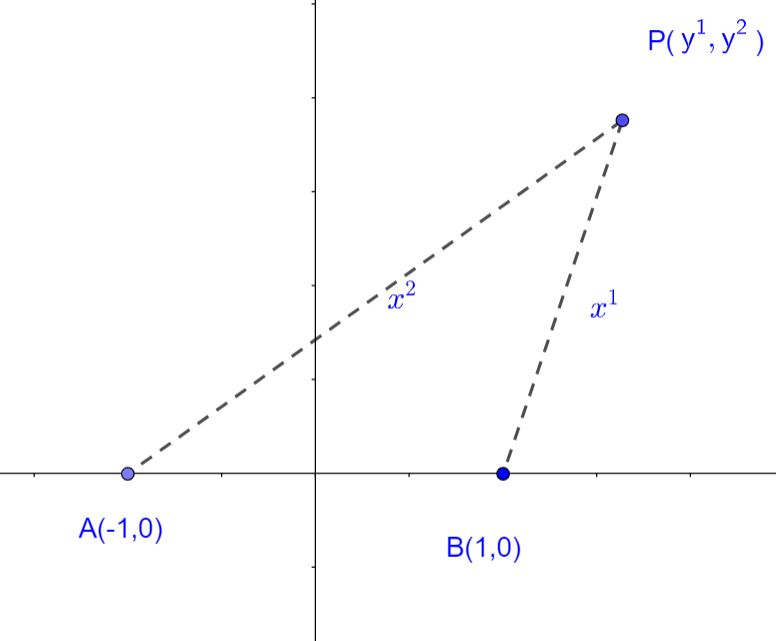
\includegraphics[scale=.4]{Bipolar.jpg}
\begin{tikzpicture}[scale=2.5]
	\coordinate  (O) at (0,0.0);
	\coordinate [label=right:$x$] (Xr) at (2.5,0);
	\coordinate  (Xl) at (-2.5,0);
	\coordinate [label=above:$y$] (Y) at (0,2.5);
		\coordinate (A) at (-1,-0);
		\coordinate  (B) at (1,0);
		\coordinate [label=above:$P \left( y^1\text{,} \  y^2 \right)$] (P) at (2,2);
		\node at ($(A) + (0,-0.3)$)    {$A \text{(-1,0 )}$};
		\node at ($(B) + (0,-0.3)$)    {$$B \text{(1,0 )}$$};
    % Draw axes
   	 \draw[ -stealth,line width = 0.25mm] (Xl) --(Xr) ;
   	 \draw[ -stealth,line width = 0.25mm] (O) --(Y) ;
   	 \draw[dashed,line width = 0.25mm] (A) --(P)node[midway,right] {$x^2$}; ;
   	  \draw[dashed,line width = 0.25mm] (B) --(P) node[midway,right] {$x^1$};
	\draw[fill=gray](A) circle(1.2pt);
	\draw[fill=gray](B) circle(1.2pt);
	\draw (P)  circle[radius=1.2pt];
\end{tikzpicture}
\caption{Bipolar coordinates}
\label{fig:fig_p79_260_a}
\end{figure}
\begin{align}
\ (x^1)^2 &= \left( y^1-1\right) ^2 + \left(y^2\right)^2\\
\ (x^2)^2 &= \left( y^1+1\right) ^2 + \left(y^2\right)^2\\
\partial_1 (1) \quad\Rightarrow \quad x^1 &= \left( y^1-1\right)\partial_1 y^1  + \left(y^2\right)\partial_1 y^2\\
\partial_2 (2) \quad\Rightarrow \quad\ x^2 &= \left( y^1+1\right)\partial_2 y^1  + \left(y^2\right)\partial_2 y^2\\
\partial_2 (1) \quad\Rightarrow \quad 0 &= \left( y^1-1\right)\partial_2 y^1  + \left(y^2\right)\partial_2 y^2\\
\partial_1 (2) \quad\Rightarrow \quad\ 0 &= \left( y^1+1\right)\partial_1 y^1  + \left(y^2\right)\partial_1 y^2\\
\Rightarrow \quad & \left\{\begin{array}{ll}
\text{(3)-(6):}& \partial_1 y^1 = -\frac{x^1}{2}\\\\
\text{(4)-(5):}& \partial_2 y^1 = \frac{x^2}{2}\\\\
\text{(6):}& \partial_1 y^2 = \frac{y^1+1}{2y^2}x^1\\\\
\text{(5):}& \partial_2 y^2 = -\frac{y^1-1}{2y^2}x^2\\
\end{array}\right.\\
\text{Hence,}\quad J &= \left(\pdv{y^m}{x^n} \right) = \begin{pmatrix}
-\frac{x^1}{2} &\frac{x^2}{2}  \\
\frac{y^1+1}{2y^2}x^1 & -\frac{y^1-1}{2y^2}x^2 \\
\end{pmatrix}
\end{align}
\newpage
Be $A$ the metric tensor in Cartesian coordinate system. Then, going to a arbitrary coordinate system gives a metric tensor according to  
\begin{align}
\ & A^, = J^TAJ =J^TJ \quad \text{as}\quad A = \begin{pmatrix}
1 &0 \\
0& 1 \\
\end{pmatrix}\\
\Rightarrow\quad & A^, = \begin{pmatrix}
-\frac{x^1}{2} & \frac{y^1+1}{2y^2}x^1 \\
\frac{x^2}{2} & -\frac{y^1-1}{2y^2}x^2 \\
\end{pmatrix}\begin{pmatrix}
-\frac{x^1}{2} &\frac{x^2}{2}  \\
\frac{y^1+1}{2y^2}x^1 & -\frac{y^1-1}{2y^2}x^2 \\
\end{pmatrix}\\
\Rightarrow\quad & A^, =\frac{x^1x^2}{4(y^2)^2} \begin{pmatrix}
\ & \\
x^1x^2 &-\left[(y^1)^2 +(y^2)^2-1)\right] \\\\
-\left[(y^1)^2 +(y^2)^2-1)\right]  &x^1x^2\\
\ & 
\end{pmatrix}
\end{align}
We use plane geometry to express expression (11) as  a function of only $(x^1,x^2)$. For the triangle $APB$ in the figure below, we have
\begin{figure}[h]
%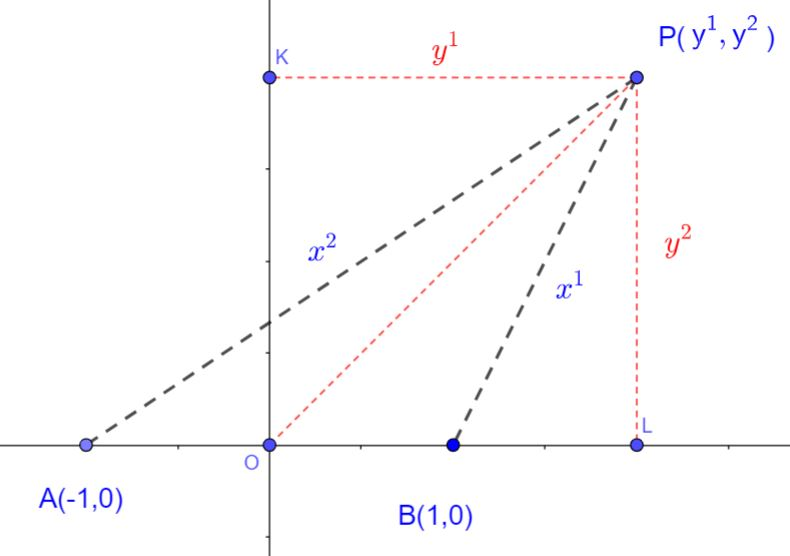
\includegraphics[scale=.4]{Bipolar2.jpg}
\begin{tikzpicture}[scale=2.5]
	\coordinate  (O) at (0,0);
	\coordinate [label=right:$x$] (Xr) at (2.5,0);
	\coordinate [label=left:$K$] (K) at (0,2);
	\coordinate (L) at (2.,0);
	\coordinate  (Xl) at (-2.5,0);
	\coordinate [label=above:$y$] (Y) at (0,2.5);
		\coordinate (A) at (-1,-0);
		\coordinate  (B) at (1,0);
		\coordinate [label=above:$P \left( y^1\text{,} \  y^2 \right)$] (P) at (2,2);
		\node at ($(A) + (0,-0.3)$)    {$A \text{(-1,0 )}$};
		\node at ($(B) + (0,-0.3)$)    {$$B \text{(1,0 )}$$};
		\node at ($(L) + (0,-0.3)$)    {$$L$$};
    % Draw axes
   	 \draw[ -stealth,line width = 0.25mm] (Xl) --(Xr) ;
   	 \draw[ -stealth,line width = 0.25mm] (O) --(Y) ;
   	 \draw[dashed,line width = 0.25mm] (A) --(P)node[midway,left] {$x^2$}; 
   	  \draw[dashed,line width = 0.25mm] (B) --(P) node[midway,right] {$x^1$};
   	   \draw[dotted,line width = 0.25mm] (O) --(P) ;
   	      	   \draw[dotted,line width = 0.25mm] (K) --(P)node[midway,above] {$y^1$}; 
   	      	      	   \draw[dotted,line width = 0.25mm] (L) --(P) node[midway,right] {$y^2$};;
	\draw[fill=gray](A) circle(1.2pt);
	\draw[fill=gray](B) circle(1.2pt);
	\draw (P)  circle[radius=1.2pt];
	\draw (K)  circle[radius=1.2pt];
	\draw (L)  circle[radius=1.2pt];
\end{tikzpicture}
\caption{Bipolar coordinates versus Cartesian coordinates}
\label{fig:fig_p79_260_b}
\end{figure}
\begin{align}
\ \left |  OP \right |^2 &= \frac{(x^1)^2+(x^2)^2}{2} - \underbrace{\frac{\left | AB \right|^2}{4}}_{=1}\\
\Rightarrow\quad (y^1)^2 +(y^2)^2 &= \frac{(x^1)^2+(x^2)^2}{2} - 1
\end{align}
The area $K$ of the triangle can be expressed in two ways
\begin{align}
\ K &= \half y^2\left | AB \right| = y^2\\
\text{and} \quad K &= \sqrt{s(s-x^1)(s-x^2)(s-2)}\\
\text{with}\quad s &= \half (x^1+x^2+2)\\
\text{hence}\quad (y^2)^2 &= \frac{1}{16}(x^1+x^2+2)(x^1+2)(x^2+2)(x^1+x^2)
\end{align}
So we get from (11):
\begin{align}
A^, =\frac{4x^1x^2}{(x^1+x^2+2)(x^1+2)(x^2+2)(x^1+x^2)} \begin{pmatrix}
\ & \\
x^1x^2 &2-\frac{(x^1)^2+(x^2)^2}{2} \\\\
2-\frac{(x^1)^2+(x^2)^2}{2}  &x^1x^2\\
\ & 
\end{pmatrix}
\end{align}
For the conjugate metric tensor we start from expression (11) and invert the metric tensor
\begin{align}
\left| A^,\right| &= \left[ \frac{x^1x^2}{4(y^2)^2}\right]^2\left[(x^1x^2)^2 -\left((y^1)^2 +(y^2)^2-1\right)^2\right]\\
\text{hence}\quad \left(a^{,mn}\right) &= \frac{1}{\left| A^,\right|}\frac{x^1x^2}{4(y^2)^2} \begin{pmatrix}
\ & \\
x^1x^2 &\left[(y^1)^2 +(y^2)^2-1\right] \\\\
\left[(y^1)^2 +(y^2)^2-1\right]  &x^1x^2\\
\ & 
\end{pmatrix}\\
\ &= \frac{4(y^2)^2\begin{pmatrix}
\ & \\
x^1x^2 &\left[(y^1)^2 +(y^2)^2-1\right] \\\\
\left[(y^1)^2 +(y^2)^2-1\right]  &x^1x^2\\
\ & 
\end{pmatrix}}{x^1x^2\left[(x^1x^2)^2 -\left((y^1)^2 +(y^2)^2-1\right)^2\right]} \\
\text{with} \quad x^1x^2&= \sqrt{\left[(y^1-1)^2 +(y^2)^2\right]\left[(y^1+1)^2 +(y^2)^2\right]}
\end{align}
$$\blacklozenge$$
\newpage

\section{p79-exercise 15}
\begin{tcolorbox}
Given $\Phi = a_{mn}dx^m dx^n$, with $a_{11} = a_{22}= 0$ but $a_{12} \ne 0$, show that $\Phi$ may be written in the form $$ \Phi = \epsilon\Psi^2_1- \epsilon\Psi^2_2 + \Phi_2$$ where $\Phi_2$ is a homogeneous quadratic form in $ dx^3, dx^4, \dots ,dx^N $, $\epsilon = \pm 1$ , and where 
$$\Psi_1 = \frac{1}{\sqrt(2 \epsilon a_{12})}\left[ a_{12}(dx^1+dx^2) + (a_{13}+a_{23})dx^3+ \dots +(a_{1N}+a_{2N})dx^N \right]$$
$$\Psi_2 = \frac{1}{\sqrt(2 \epsilon a_{12})}\left[ a_{12}(-dx^1+dx^2) + (a_{13}-a_{23})dx^3+ \dots +(a_{1N}-a_{2N})dx^N \right]$$
\end{tcolorbox}
Using local Cartesian coordinates we have:
Be 
\begin{align}
\Phi &= a_{mn}dx^mdx^n\\ 
\end{align}
and consider the following sequences of terms: 
\begin{align}
\Psi_1 =  b_{11}dx^1+b_{12}dx^2 + b_{13}dx^3+ \dots +b_{1N}dx^N \\
\Psi_2 =  b_{21}dx^1+b_{22}dx^2 + b_{23}dx^3+ \dots +b_{2N}dx^N 
\end{align}
The expressions (3) and (4) contain all the terms of $\Phi$ with $(dx^1)^2,(dx^2)^2$ and $dx^1dx^2$. So, $\Phi$ can be expressed as 
\begin{align}
\Phi =\Psi_1^2 -\Psi_2^2 + \Phi_2 
\end{align}
With $\Phi_2 $ being a homogeneous form containing only terms in $dx^i dx^j \quad i,j > 2$.\\
We can express $\Psi_1^2 - \Psi_2^2$ as
\begin{align}
\Psi_1^2 - \Psi_2^2 &= \left \{ \begin{array}{l}(b_{11}^2 - b_{21}^2)(dx^1)^2 +(b_{12}^2 - b_{22}^2)(dx^2)^2 +(b_{13}^2 - b_{23}^2)(dx^3 )^2 + \dots +(b_{1N}^2 - b_{2N}^2)(dx^N)^2 +\\
 2( b_{11} b_{12}-b_{21} b_{22})dx^1dx^2+2( b_{11} b_{13}-b_{21} b_{23})dx^1dx^3+\dots + 2( b_{11} b_{1N}-b_{21} b_{2N})dx^1dx^N+\\
 2( b_{12} b_{13}-b_{22} b_{23})dx^2dx^3+2( b_{12} b_{14}-b_{22} b_{24})dx^2dx^4+\dots + 2( b_{12} b_{1N}-b_{21} b_{2N})dx^2dx^N+\\
 + \dots 2( b_{1j} b_{1k}-b_{2j} b_{2k})dx^kdx^j+\dots\quad j>2, \ k\ne j
\end{array} \right.
\end{align}
Equating the terms in (1) and (6) and taking into account (=given) $a_{11}=a_{22}=0$ and $a_{12} \ne0$ 
\begin{align}
\ &\left \{ \begin{array}{l}
 b_{11}^2 - b_{21}^2 =0\\
 b_{12}^2 - b_{22}^2 =0\\
 2\left(b_{11}b_{12} - b_{21}b_{22} \right) = a_{12}+a_{21}
\end{array}\right.\\
\Rightarrow \quad \ &\left \{ \begin{array}{l}
 b_{11}^2 = b_{21}^2 \\
 b_{12}^2 = b_{22}^2 \\
 \left(b_{11}b_{12} - b_{21}b_{22} \right) =a_{12}
\end{array}\right.\\
\Rightarrow\quad b_{11} = \pm b_{21}  &\quad b_{22} =\pm b_{12}\\ 
\Rightarrow\quad  &\left \{ \begin{array}{l} 
 \pm b_{11}b_{22} \mp b_{11}b_{22}  =a_{12}\\ 
\text{or}\\
\pm b_{12}b_{21} \mp b_{12}b_{21}  =a_{12}
\end{array}\right.\\
\end{align}
As $a_{12} \ne0$, the signs in the above expressions must be the same. Hence,
\begin{align}
&\left \{ \begin{array}{c} 
 2b_{11}b_{22} =\pm a_{12}\\ 
2 b_{12}b_{21} =\pm a_{12} 
\end{array}\right.
\end{align}
(12) can be satisfied with an infinite combination of $b_{11},b_{12},b_{21}, b_{22}$. Choose,
\begin{align} 
\ b_{11} = \sqrt{\frac{\epsilon a_{12}}{2 }}\quad b_{22} = \sqrt{\frac{\epsilon a_{12}}{2 }}\quad & b_{12} = \sqrt{\frac{\epsilon a_{12}}{2 }}\quad b_{21} = - \sqrt{\frac{\epsilon a_{12}}{2 }}\\
\text{with} \quad  \epsilon &= \pm 1\quad\text{so that}\quad \epsilon a_{12} \geq 0
\end{align}
Put $\xi = \sqrt{\frac{\epsilon a_{12}}{2 }}$. Then, (3) and (4) can be expressed as 
\begin{align}
\Psi_1 =  \xi dx^1+\xi dx^2 + b_{13}dx^3+ \dots +b_{1N}dx^1dx^N \\
\Psi_2 =  -\xi dx^1+\xi dx^2 + b_{23}dx^3+ \dots +b_{2N}dx^1dx^N 
\end{align}
What are the $b_{.j}\quad (j>2)$? \\From (6), e.g. for $j=3$,  identifying the terms in $dx^1dx^3$ and $dx^2dx^3$ we see that
\begin{align}
&\left \{ \begin{array}{l} 
 \xi b_{13}+\xi b_{23} =a_{13}\\ 
\xi b_{13}-\xi b_{23} =a_{23}\\ 
\end{array}\right.\\
\Rightarrow \quad &\left \{ \begin{array}{l} 
 b_{13}=\frac{a_{13}+a_{23}}{2\xi}\\ 
 b_{23}=\frac{a_{13}-a_{23}}{2\xi}
\end{array}\right.\\
\text{or, in general} \quad &\left \{ \begin{array}{ll} 
 b_{1j}=\frac{a_{1j}+a_{2j}}{2\xi}\\
 \ &\ (j>2)\\ 
 b_{2j}=\frac{a_{1j}-a_{2j}}{2\xi}
\end{array}\right.
\end{align}
Bring $\frac{1}{\xi}$ out in $\Psi_1, \Psi_2$. This gives
\begin{align}
\Psi_1 &= \frac{1}{\xi}\left( \xi^2( dx^1+ dx^2) + \frac{a_{13}+a_{23}}{2}dx^3+ \dots +\frac{a_{1N}+a_{2N}}{2}dx^N \right) \\
\Psi_2 &= \frac{1}{\xi}\left( \xi^2(- dx^1+ dx^2) + \frac{a_{13}-a_{23}}{2}dx^3+ \dots +\frac{a_{1N}-a_{2N}}{2}dx^N \right) \\
\Rightarrow \quad &\left \{ \begin{array}{l} 
\Psi_1 = \frac{\sqrt{2}}{\sqrt{\epsilon a_{12}}}\left( \frac{\epsilon a_{12}}{2 } (dx^1+ dx^2) + \frac{a_{13}+a_{23}}{2}dx^3+ \dots +\frac{a_{1N}+a_{2N}}{2}dx^N \right) \\\\
\Psi_2 = \frac{\sqrt{2}}{\epsilon\sqrt{\epsilon a_{12}}}\left( \frac{\epsilon a_{12}}{2 } (-dx^1+ dx^2) + \frac{a_{13}-a_{23}}{2}dx^3+ \dots +\frac{a_{1N}-a_{2N}}{2}dx^N \right) \\
\end{array}\right.\\
\Leftrightarrow \quad &\left \{ \begin{array}{l} \\
\Psi_1 = \frac{1}{\sqrt{2 \epsilon a_{12}}}\left(\epsilon a_{12}(dx^1+ dx^2) + (a_{13}+a_{23})dx^3+ \dots +(a_{1N}+a_{2N})dx^N \right) \\\\
\Psi_2 = \frac{1}{\sqrt{2 \epsilon a_{12}}}\left( \epsilon a_{12}(- dx^1+ dx^2) + (a_{13}-a_{23})dx^3+ \dots +(a_{1N}-a_{2N})dx^N \right) \\
\end{array}\right.
\end{align}
What about the factor $\epsilon = \pm1$ in the terms $\epsilon a_{12}(dx^1+ dx^2)$ and $\epsilon a_{12}(-dx^1+ dx^2)$ ? Consider the alternate form
\begin{align}
\ &\left \{ \begin{array}{l} \\
\Psi^,_1 = \frac{1}{\sqrt{2 \epsilon a_{12}}}\left( a_{12}(dx^1+ dx^2) + (a_{13}+a_{23})dx^3+ \dots +(a_{1N}+a_{2N})dx^N \right) \\\\
\Psi^,_2 = \frac{1}{\sqrt{2 \epsilon a_{12}}}\left(  a_{12}(- dx^1+ dx^2) + (a_{13}-a_{23})dx^3+ \dots +(a_{1N}-a_{2N})dx^N \right) \\
\end{array}\right.
\end{align}
Let's have a look at the terms in $dx^idx^j$ in $\Psi_1^{,2}-\Psi^{,2}_2$\\
\begin{align}
\ x_{11}(dx^1)^2+ 2x_{12}dx^1dx^2+x_{22}(dx^2)^2&= \frac{1}{2 \epsilon a_{12}}\left(( a_{12})^2(dx^1 + dx^2)^2 - ( a_{12})^2(-dx^1 + dx^2)^2\right)  \\
&= \frac{\epsilon a_{12}}{2}\left((dx^1 +  dx^2)^2 - (- dx^1 + dx^2)^2\right)  \\
&= \frac{\epsilon a_{12}}{2}\left((dx^1)^2 + 2 dx^1dx^2+  (dx^2)^2 - (dx^1)^2 + 2 dx^1dx^2-  (dx^2)^2\right)  \\
&= 2 \epsilon a_{12}dx^1dx^2 \\
\ 2x_{13}dx^1dx^3&= \frac{1}{2 \epsilon a_{12}}(2 a_{12}(a_{13}+a_{23})dx^1dx^3 - 2a_{12}(a_{13}-a_{23})dx^1dx^3) \\
\ &= \frac{1}{2 \epsilon a_{12}}(4 a_{12}a_{23})dx^1dx^3 \\
 & =  2\epsilon a_{23}dx^1dx^3\\
 \ 2x_{23}dx^2dx^3&= \frac{1}{2 \epsilon a_{12}}(2 a_{12}(a_{13}+a_{23})dx^1dx^3 - 2 a_{12}(a_{13}-a_{23})dx^1dx^3) \\
\ &= \frac{1}{2 \epsilon a_{12}}(4 a_{12}a_{23})dx^1dx^3 \\
 & =  2\epsilon a_{23}dx^1dx^3\\
\ 2x_{34}dx^3dx^4&=  \frac{1}{2 \epsilon a_{12}}\left(\begin{array}{l} 2 (a_{13}+ a_{23})(a_{14}+ a_{24}\\ - 2 (a_{13}- a_{23})(a_{14}- a_{24}) \end{array} \right)dx^3dx^4 \\
\ &= \frac{2\epsilon}{ a_{12}}\left(a_{23}a_{14}+a_{13}a_{24}\right)
\end{align}
We rewrite now the metric form $\Phi$ as 
$$\Phi =\epsilon \Psi_1^{,2}- \epsilon \Psi^{,2}_2 + \Phi_2 $$
From (28), (31) and (34) we see that the terms in $dx^1, dx^2$ in $\Phi =\epsilon \Psi_1^{,2}- \epsilon \Psi^{,2}_2 + \Phi_2$ correspond to the expected  metric form and that the other terms in $dx^j, dx^k, \ j,k \neq 1,2$ can be corrected in the remaining term $\Phi_2$.
\newpage

\section{p80-exercise 16}
\begin{tcolorbox}
Find the null geodesics of a 4-space with line element
$$ds^2=\epsilon \gamma\left(dx^2 +dy^2+dz^2-dt^2\right)$$ where $\gamma$ is an arbitrary function of $x,\ y,\ z,\ t$.
\end{tcolorbox}
We have:
\begin{align}
\left(a_{mn}\right) = \gamma\begin{pmatrix}
 1&0  & 0 & 0 \\
 0&  1& 0 & 0 \\
 0&0  & 1 &  0\\
 0& 0 & 0 & -1 \\
\end{pmatrix} \quad \left(a^{mn}\right) = \frac{1}{\gamma}\begin{pmatrix}
 1&0  & 0 & 0 \\
 0&  1& 0 & 0 \\
 0&0  & 1 &  0\\
 0& 0 & 0 & -1 \\
\end{pmatrix}\\
\end{align}
Be $(x^1,x^2,x^3,x4) \equiv (x,y,z,t)$.\\
The general conditions for a null geodesic are
\begin{align}
\left \{ \begin {array}{l}
\dv[2]{x^r}{v} + \Gamma^r_{mn}\dv{x^m}{v}\dv{x^n}{v} = 0\\\\
\ a_{mn}dx^mdx^n =0
\end{array}\right.
\end{align}
When calculating $[mn,r] = \half\left(\partial_n a_{mr}+\partial_m a_{nr}-\partial_r a_{mn} \right) $ we note that $\left(a_{mn}\right)$ is a diagonal matrix, ans so is also $\left(a^{mn}\right)$. Hence $\Gamma^r_{mn}$ will contain only one term:
\begin{align}
\ & \Gamma^r_{mn} = a^{RR}[mn,R]\\
\Rightarrow \quad & \left \{ \begin{array}{llll}
\ i)& m,n \neq R \ \wedge \ m \neq n&:& [mn,R]=0\\\\
\ ii)& m \neq n = R \ \vee \  n \neq m = R&:& [mn,R]=\half \partial_m a_{RR}\\\\
\ iii)& m =n \neq R &:& [mn,R]=-\half \partial_R a_{mn}\\\\
\ iv)& m =n= R &:& [mn,R]=\half \partial_R a_{RR}\\\\
\end{array}\right.
\end{align}\\
and for the $\Gamma^r_{mn}$:\\
\begin{align}
\Rightarrow \quad & \left \{ \begin{array}{llll}
\ i)& m,n \neq R \ \wedge \ m \neq n &:& \Gamma^R_{mn}=0\\\\
\ ii)& m \neq n = R \ \vee \  n \neq m = R &:& \Gamma^R_{nR}=\frac{1}{2 \gamma} \partial_n \gamma \\\\
\ iii)& m =n \neq R = \ 1,2,3 &:& \Gamma^R_{kk}=-\frac{1}{2 \gamma}  \partial_R \gamma\\
\ & m =n \neq R =4 &:& \Gamma^4_{kk}=\frac{1}{2 \gamma}  \partial_R \gamma\\\\
\ iv)& m =n= R &:& \Gamma^R_{RR}=\frac{1}{2 \gamma}  \partial_R \gamma\\\\
\end{array}\right.
\end{align}
Let's compute 
\begin{align}
\ A_r \equiv \dv[2]{x^r}{v} + \Gamma^r_{mn}\dv{x^m}{v}\dv{x^n}{v}
\end{align}
and take $v = x^4$, so $x^1, \  x^2,  \ x^3 = f(x^4)$. (In the following $d_kx^j \equiv \dv{x^j}{{(x^{k})}}\ , \ d^2_kx^j \equiv \dv[2]{x^j}{{(x^{k})}}$)
\begin{align}
\left \{ \begin{array}{ll}
\ A_1 = &  d^2_4x^1+ \Gamma^1_{mn}d_4x^md_4x^n\\
\ A_2 = &  d^2_4x^2+ \Gamma^2_{mn}d_4x^md_4x^n\\
\ A_3 = &  d^2_4x^3+ \Gamma^3_{mn}d_4x^md_4x^n\\
\ A_4 = &   \Gamma^4_{mn}d_4x^md_4x^n
\end{array} \right.
\end{align}
and get from (8) and (6):
\begin{align}
\ A_1 -d^2_4x^1 &= \left \{ \begin{array}{l}\frac{1}{\gamma}  \partial_2 \gamma \ d_4x^1d_4x^2  + \frac{1}{\gamma}  \partial_3 \gamma \ d_4x^1 d_4x^3+\frac{1}{\gamma}  \partial_4 \gamma \ d_4x^1 d_4x^4\\\\
\ + \underbrace{\frac{1}{2\gamma}\partial_1 \gamma (d_4x^1)^2}_{= \left \{ \begin{array}{l} \frac{1}{\gamma} \partial_1 \gamma (d_4x^1) (d_4x^1)\\
\  - \frac{1}{2\gamma} \partial_1 \gamma (d_4x^1)^2 \end{array} \right.} - \frac{1}{2\gamma}\partial_1 \gamma (d_4x^2)^2- \frac{1}{2\gamma}\partial_1 \gamma (d_4x^3)^2+ \frac{1}{2\gamma}\partial_1 \gamma (d_4x^4)^2
 \end{array} \right.\\
 &= \left \{ \begin{array}{l}\frac{1}{\gamma} \partial_1 \gamma d_4x^1 d_4x^1 + \frac{1}{\gamma}  \partial_2 \gamma \ d_4x^1d_4x^2  + \frac{1}{\gamma}  \partial_3 \gamma \ d_4x^1 d_4x^3+\frac{1}{\gamma}  \partial_4 \gamma \ d_4x^1 d_4x^4\\\\
\ - \frac{1}{2\gamma}\partial_1 \gamma (d_4x^1)^2 - \frac{1}{2\gamma}\partial_1 \gamma (d_4x^2)^2- \frac{1}{2\gamma}\partial_1 \gamma (d_4x^3)^2+ \frac{1}{2\gamma}\partial_1 \gamma (d_4x^4)^2
 \end{array} \right.\\\\
  &= \left \{ \begin{array}{l}\frac{1}{\gamma}d_4x^1 \left(\partial_1 \gamma  d_4x^1  + \partial_2 \gamma \ d_4x^2  + \partial_3 \gamma \  d_4x^3+ \partial_4 \gamma \ d_4x^4 \right)\\\\
\ - \frac{1}{2\gamma}\partial_1 \gamma \left(\underbrace{(d_4x^1)^2 +(d_4x^2)^2+(d_4x^3)^2- (d_4x^4)^2}_{= a_{mn}dx^m dx^n = 0 }\right)
 \end{array} \right.\\
 \Rightarrow \quad A_1 &= d^2_4x^1+ \frac{1}{\gamma}d_4x^1 < \grad \gamma|\partial_4 \overline{x} >
\end{align}
with $\grad \gamma =  (\partial_x \gamma,\ \partial_y \gamma, \ \partial_z \gamma, \ \partial_t \gamma)$ and $ \partial_4 \overline{x} =  (\partial_t x, \ \partial_t y , \ \partial_t z, \ \partial_t t)$.\\
So for the geodesic with get for the first coordinate $$d^2_4x^1+ \frac{1}{\gamma}d_4x^1 < \grad \gamma|\partial_4 \overline{x} > = 0 $$
Doing analogous calculations give the following set of equations
\begin{align}
\ d^2_4x^k+ \frac{1}{\gamma}d_4x^k < \grad \gamma|\partial_4 \overline{x} > = 0 
\end{align}
Note that for $k=4$ we have as $\ d_4x^4 = 1$ and $\ d^2_4x^4 = 0$:
\begin{align}
 \frac{1}{\gamma}< \grad \gamma|\partial_4 \overline{x} > = 0 \\
 \Rightarrow \quad < \grad \gamma|\partial_4 \overline{x} > = 0 
\end{align}
Note that this means that $\grad \gamma$ and $\partial_4 \overline{x}$ are orthogonal 4-vectors.\\
So the set of equations in (14) reduce to the following set of $2^{nd}$ order differential equations:
\begin{align}
\ & \left  \{ \begin{array}{l}
\ x^{,,} = 0\\
\ y^{,,} = 0\\
\ z^{,,} = 0\\
\ t = t\\
\end{array} \right.
\Rightarrow  \left  \{ \begin{array}{l}
\ x = x_1t+x_0\\
\ y =y_1t+y_0\\
\ z = z_1t+z_0\\
\ t = t\\
\end{array} \right.
\end{align}
This is the equations of 4-space cone, which was expected as the metric is localy a Minkowksi-like metric. 
$$\blacklozenge$$
\newpage

\section{p80-exercise 17}
\begin{tcolorbox}
In a space $V_N$ the metric tensor is $a_{mn}$. Show that the null geodesics are unchanged if the metric tensor is changed to $b_{mn} = \gamma a_{mn} $, $\gamma$ being a function of the coordinates.
\end{tcolorbox}
Null geodesics are determined by the following set of equations
\begin{align}
\ & \left \{  \begin {array}{l}
\dv[2]{x^r}{v} + \Gamma^r_{mn}\dv{x^m}{v}\dv{x^n}{v} = 0\\\\
\ a_{mn}dx^mdx^n =0
\end{array}\right.\\
\text{We have}\quad  \Gamma^r_{mn} & = a^{rs}[mn,s]\\
\ & = \frac{1}{\gamma}a^{rs}\gamma[mn,s]\\
\text{We have also }\quad  b^{rs} & = \frac{1}{\gamma}a^{rs}\\
\text{Indeed }\quad  a^{rs}a_{rs}&= \delta^r_t\\
\Rightarrow\quad  \frac{1}{\gamma}a^{rs}\gamma a_{rs}&= \delta^r_t\\
\Rightarrow\quad  \frac{1}{\gamma}a^{rs}b_{rs}&= \delta^r_t\\
\Rightarrow\quad  \frac{1}{\gamma}a^{rs} &= b_{rs}\\
\text{So (3) becomes}\quad  \Gamma^r_{mn} & =b^{rs}\gamma[mn,s]
\end{align}
Be $ [mn,s]^{'} $ the Christoffel symbol associated with the metric $b_{mn}= \gamma a_{mn}$. Then with  $$[mn,s]^, = \half \left(\partial_n \gamma a_{ms}+\partial_m \gamma a_{ns}-\partial_s \gamma a_{mn} \right)$$ we get
\begin{align}
\ [mn,s]^{'} &= \gamma [mn,s] + \half\left( a_{ms}\partial_n \gamma+a_{ns}\partial_m \gamma-a_{mn}\partial_s \gamma \right)
\end{align}
Substitute $\gamma [mn,s]$ from (10) in (9) we get
\begin{align}
\Gamma^r_{mn} & =\underbrace{b^{rs}\gamma[mn,s]^,}_{=\Gamma^{'r}_{mn}}  - \underbrace{\half b^{rs}\left( a_{ms}\partial_n \gamma+a_{ns}\partial_m \gamma-a_{mn}\partial_s \gamma \right)}_{\coloneqq Q}\\
\text{with}\quad Q &= \half b^{rs}\left( a_{ms}\partial_n \gamma+a_{ns}\partial_m \gamma-a_{mn}\partial_s \gamma \right)\\
&= \half \gamma \left( \underbrace{a^{rs}a_{ms}}_{ = \delta^r_m}\partial_n \gamma+\underbrace{a^{rs}a_{ns}}_{ = \delta^r_n}\partial_m \gamma-a^{rs}a_{mn}\partial_s \gamma \right)\\
\ Q \times \dv{x^m}{v}\dv{x^n}{v} &= \half \gamma \left( \underbrace{\delta^r_m\dv{x^m}{v}}_{=\dv{x^r}{v}} \underbrace{\partial_n \gamma \dv{x^n}{v}}_{= \dv{\gamma}{v}}+\underbrace{\delta^r_n\dv{x^n}{v}}_{=\dv{x^r}{v}}\underbrace{\partial_m \gamma\dv{x^m}{v}}_{= \dv{\gamma}{v}}-a^{rs}\partial_s \gamma \underbrace{a_{mn}\dv{x^m}{v}\dv{x^n}{v}}_{ = 0 \ \text{by(1)}} \right)\\
&= \half \gamma \left( \dv{x^r}{v}\dv{\gamma}{v} +\dv{x^r}{v}\dv{\gamma}{v} \right)\\
&= \left(\gamma\dv{\gamma}{v} \right)  \dv{x^r}{v}
\end{align}
So from (11) and (16), (1) can be expressed as 
\begin{align}
\dv[2]{x^r}{v} + \Gamma^{'r}_{mn}\dv{x^m}{v}\dv{x^n}{v} = \left(\gamma\dv{\gamma}{v} \right)  \dv{x^r}{v}
\end{align}
By (2.449) page 46 we see that the vector 
$\dv[2]{x^r}{v} + \Gamma^{'r}_{mn}\dv{x^m}{v}\dv{x^n}{v}$ is collinear to $\dv{x^r}{v}$. Also $b_{mn}\dv{x^m}{v}\dv{x^n}{v} = 0$. And hence (17) determines the geodesic null lines. So both expressions (1) and (17) are equivalent to determine the same geodesic null lines in the space $V_N$ equipped with the metric $a_{mn}$ or  $b_{mn}$
$$\blacklozenge$$
\newpage


\section{p80-exercise 18}
\begin{tcolorbox}
Are the relations $$T_{|rs} =T_{|sr} $$ $$T_{r|sk} =T_{r|ks} $$ true (a) in curvilinear coordinates in Euclidean space, (b) in a general Riemannian space?
\end{tcolorbox}
$$\boldsymbol{T_{|rs} \questeq  T_{|sr}}$$
We have $T|_r = \partial_rT$ (see (2.528) page 53) \\
\begin{equation}
  \begin{split}
  \ & \boldsymbol{T_{|rs}}\\\\
   \ & T|_{rs} = \partial^2_{rs}T - \Gamma^m_{rs}T|_m
  \end{split}
\quad\leftrightarrow\quad
  \begin{split}
 \ & \boldsymbol{T_{|sr}}\\\\
   \ & T|_{sr} = \partial^2_{sr}T - \Gamma^m_{sr}T|_m
  \end{split}
\end{equation}
As $\partial^2_{rs} =\partial^2_{sr}$ and $\Gamma^m_{rs} =\Gamma^m_{sr}$ we can conclude that $\boldsymbol{T_{|rs} =T_{|sr}}$ in both cases (a) and (b).\\\\
$$\boldsymbol{\diamond}$$\\\\
$$\boldsymbol{T_{r|sk} \questeq  T_{r|ks}}$$
\begin{equation}
  \begin{split}
  \ & \boldsymbol{T_{r|sk}}\\\\
  \ & A_{rs} \coloneqq T_{r|s} = \partial_{s}T_r - \Gamma^m_{rs}T_m\\
  \ & A_{rs|k}= \partial_k A_{rs} - \Gamma^m_{rk}A_{ms} -  \Gamma^m_{sk}A_{rm}\\
  \ & A_{ms}=  \partial_{s}T_m - \Gamma^n_{ms}T_n\\
  \ & A_{rm} = \partial_{m}T_r - \Gamma^n_{rm}T_n\\
  \ & A_{rs|k}= \left \{\begin{array}{l}
   \underbrace{\partial^2_{sk}T_r}_{*} - T_m\partial_{k}\Gamma^m_{rs} - \underbrace{\Gamma^m_{rs}\partial_{k}T_m}_{**} \\\\
   \ -\underbrace{\Gamma^m_{rk}\partial_{s}T_m}_{***} +\Gamma^m_{rk} \Gamma^n_{ms}T_n \\\\
   \ - \underbrace{\Gamma^m_{sk}\partial_{m}T_r}_{****} +\underbrace{\Gamma^m_{sk} \Gamma^n_{rm}T_n}_{*****}
  \end{array}\right.
  \end{split}
\quad\leftrightarrow\quad
  \begin{split}
 \ & \boldsymbol{T_{r|sk}}\\\\
  \ & B_{rk} \coloneqq T_{r|k} = \partial_{k}T_r - \Gamma^m_{rk}T_m\\
  \ & B_{rk|s}= \partial_s B_{rk} - \Gamma^m_{rs}B_{mk} -  \Gamma^m_{ks}B_{rm}\\
  \ & B_{mk}=  \partial_{k}T_m - \Gamma^n_{mk}T_n\\
  \ & B_{rm}=  \partial_{m}T_r - \Gamma^n_{rm}T_n\\
  \ & B_{rk|s}= \left \{\begin{array}{l}
  \underbrace{\partial^2_{ks}T_r}_{*} - T_m\partial_{s}\Gamma^m_{rk} - \underbrace{\Gamma^m_{rk}\partial_{s}T_m}_{***} \\\\
   \ -\underbrace{\Gamma^m_{rs}\partial_{k}T_m}_{**} +\Gamma^m_{rs} \Gamma^n_{mk}T_n \\\\
   \ - \underbrace{\Gamma^m_{ks}\partial_{m}T_r}_{****} +\underbrace{\Gamma^m_{ks} \Gamma^n_{rm}T_n}_{*****}
  \end{array}\right.
  \end{split}
\end{equation}\begin{align}
\Rightarrow\quad A_{rs|k} - B_{rk|s} &= T_m\left( \underbrace{\partial_{s}\Gamma^m_{rk}-\partial_{k}\Gamma^m_{rs}+\Gamma^n_{rk} \Gamma^m_{ns}- \Gamma^n_{rs} \Gamma^m_{nk} }_{\coloneqq R^s{.rmn}}\right) 
\end{align}
So, $T_{r|sk} =  T_{r|ks}$ only if $T_m R^s_{.rmn} = 0$ and as $T_m$ is an arbitrary tensor, $R^s_{.rmn}$ must vanish for $T_{r|sk} =  T_{r|ks}$.\\\\
$\textbf{Note:}$\\
Although $\Gamma^n_{rk}$ is not a tensor, the quantity $R^s_{.rmn}$ is. Indeed, as both $A_{rs|k} - B_{rk|s}$ and $ T_m$ have the tensor character, this implies that $R^s_{.rmn}$ is a tensor.
Now, for an Euclidean space equipped with Cartesian coordinates all $\Gamma^n_{rk} $ are constant and vanish. So, $R^s_{.rmn}$ = 0. Let's consider a change of coordinate system from Cartesian to curvilinear coordinate system. Then, by the tensor character of $R^{'a}_{\ .bcd}$ we have,
\begin{align}
\ R^{'a}_{\ .bcd} = R^s_{.rmn}\partial_s x^{'a} \partial_{('b)} x^{r} \partial_{('c)} x^{m} \partial_{('d)} x^{n}
\end{align}
but $R^s_{.rmn} =0$ in the Cartesian coordinate system and so is $R^{'a}_{\ .bcd}$\\
$\textbf{Conclusion:}$\\
In a general Riemannian space $T_{r|sk} \neq  T_{r|ks}$ but $T_{r|sk} =  T_{r|ks}$ in a curvilinear Euclidean space.
$$\blacklozenge$$
\newpage

\section{p80-exercise 19}
\begin{tcolorbox}
Consider a $V_N$ with indefinite metric form. For all points $P$ lying on the cone of  geodesic null lines drawn from  $O$, the definition 2.611 for Riemannian coordinates apparently breaks down. Revise the definition of Riemannian coordinates so as to include such points.
\end{tcolorbox}
For geodesic null lines we have (2.445 page 46)
\begin{align}
\left \{ \begin{array}{l}
\dv[2]{x^r}{u} + \Gamma^r_{mn}\dv{x^m}{u}\dv{x^n}{u} = 0\\
\ a_{mn}\dv{x^m}{u}\dv{x^n}{u} = 0
\end{array}\right.
\end{align}
or (2.448 page 46)
\begin{align}
\left \{ \begin{array}{l}
\dv[2]{x^r}{v} + \Gamma^r_{mn}\dv{x^m}{v}\dv{x^n}{v} = \lambda(v) \dv{x^r}{v}\\
\ a_{mn}\dv{x^m}{v}\dv{x^n}{v} = 0
\end{array}\right.
\end{align}
where by suitable choice of the parameter $v$ , $\lambda(v) $ can be made any preassigned function of $v$.
\begin{align}
\text{(2)} \RAr \dv[2]{x^r}{v} &=   \lambda \dv{x^r}{v}-\Gamma^r_{mn}\dv{x^m}{v}\dv{x^n}{v} \\
\RAr \dv[3]{x^r}{v} &=   \dv{\lambda }{v}\dv{x^r}{v}+ \lambda \dv[2]{x^r}{v}+ A^r_{.mns}\dv{x^m}{v}\dv{x^n}{v}\dv{x^s}{v} \\
\text{with}\RAr A^r_{.mns} &= - \partial_s \Gamma^r_{mn} + 2 \Gamma^r_{sp}\Gamma^p_{mn}
\end{align}
Expanding $x^r$ in a Taylor series around a point $O(a^r)$ we get (for ease of notation we put $p^r \coloneqq \dv{x^r}{v}$)
\begin{align}
\ x^r &= a^r + v p^r + \half v^2\lambda  p^r -  \half v^2\Gamma^r_{mn}p^mp^n+\frac{1}{6}v^3\dv{\lambda  }{v}p^r + \frac{1}{6}v^3\lambda  \dv{p^r}{v} + \frac{1}{6}v^3A^r_{.mns}p^mp^np^s+\dots\\
&= a^r + \left(v  + \half v^2\lambda  +\frac{1}{6}v^3\dv{\lambda  }{v}\right)p^r -  \half v^2\Gamma^r_{mn}p^mp^n + \frac{1}{6}v^3\lambda  \dv{p^r}{v} + \frac{1}{6}v^3A^r_{.mns}p^mp^np^s+\dots
\end{align}
Put $x^{'r} \coloneqq   v\xi(v) p^r$ with $\xi(v) = \left(1  + \half v\lambda  +\frac{1}{6}v^2\dv{\lambda  }{v}\right)$. Hence (7) becomes
\begin{align}
\ x^r &= a^r + x^{'r} + \frac{\lambda v^3}{6}  \left( \frac{p^{'r}}{v\xi} - \frac{\xi + v\xi^{'}}{v^2\xi^2}x^{'r}\right)  -  \frac{\Gamma^r_{mn}}{2\xi ^2}x^{'m}x^{'n} + \frac{A^r_{.mns}}{6\xi ^3}x^{'m}x^{'n}x^{'s}+\dots\\
\ & = a^r + \tau(v) x^{'r}+ \frac{\lambda v^2 }{6\xi}p^{'r} -  \frac{\Gamma^r_{mn}}{2\xi ^2}x^{'m}x^{'n}   + \frac{A^r_{.mns}}{6\xi ^3}x^{'m}x^{'n}x^{'s}+\dots\\
\text{with}\spatie & \tau(v)  \coloneqq 1-\frac{\lambda v}{6\xi^2}\left( \xi + v\xi^{,}\right)
\end{align}\\
Is the Jacobian non-zero?
\begin{align}
\pdv{x^r}{x^{'q}}  & = \tau\delta^r_q+ \frac{\lambda  v^2}{6\xi}\dv{\delta^r_q}{v} -  \frac{\Gamma^r_{mq}}{\xi ^2}x^{'m}   + \frac{A^r_{.mnq}}{2\xi ^3}x^{'m}x^{'n}+\dots
\end{align}
In the infinitesimal neighbourhood of $O$ we have \\
\begin{align}\left \{ \begin{array}{l} 
v \rightarrow 0\\  
\xi \rightarrow 1\\
\xi^{'} \rightarrow \frac{\lambda }{2}\\ 
x^{'m} \rightarrow 0\\
\tau \rightarrow 1 
\end{array} \right.\\
\end{align}
so that the Jacobian determinant becomes
\begin{align}
\left| \pdv{x^r}{x^{'q}} \right| &= \left| \tau\delta^r_q \right| =\tau ^N = 1
\end{align}
$\textbf{Conclusion:}$\\
So in order to define a Riemannian coordinates system which is still valid on the null geodesics, it is sufficient to define the Riemannian coordinates around $O$ as $$ x^{'r} \coloneqq   v\xi p^r$$ with $$\xi(v) = \left(1  + \frac{\lambda}{2} v +\frac{1}{6}\dv{\lambda }{v} v^2\right) $$
and $\lambda $, by suitable choice of $v$, being any pre-defined function of $v$.
$$\blacklozenge$$
\newpage
